% ---- ETD Document Class and Useful Packages ---- %
\documentclass{ucetd}
\usepackage{subfigure,epsfig,amsfonts}
\usepackage{natbib}
\usepackage{amsmath}
\usepackage{amssymb}
\usepackage{amsthm}
% Add extra packages I need
\usepackage{fixltx2e}
\usepackage{longtable}
\usepackage{booktabs}
\usepackage[breaklinks]{hyperref}
\renewcommand{\etdChapterHeadFormat}[1]{\uppercase{#1}}


%% Use these commands to set biographic information for the title page:
\title{Transcriptomic approaches to investigate tuberculosis susceptibility}
\author{John D. Blischak}
\department{Committee on Genetics}
\division{Biological Sciences Division}
\degree{Doctor of Philosophy}
\date{December 2016}

%% Use these commands to set a dedication and epigraph text
\dedication{Dedication Text}
\epigraph{Epigraph Text}


\begin{document}
%% Basic setup commands
% If you don't want a title page comment out the next line and uncomment the line after it:
\maketitle
%\omittitle

% These lines can be commented out to disable the copyright/dedication/epigraph pages
\makecopyright
%\makededication
%\makeepigraph


%% Make the various tables of contents
\tableofcontents
\listoffigures
\listoftables

\acknowledgments
% Enter Acknowledgements here

% Enter Abstract here
\abstract
A primary aim of the human genetics is to determine how genetic variation impacts phenotypic variation, including in complex traits and diseases. Understanding this relationship will ultimately allow the field understand the molecular basis of complex traits and better diagnose and treat human diseases. To dissect this relationship, human geneticists have leveraged comparisons between humans and other primates, as well as between different groups of humans. To maximize the utility of these functional genomics studies, proper study design must be deployed. Indeed, the primate comparative studies in Chapters 2 and 3 highlight study design challenges and potential solutions. Furthermore, this work demonstrates that adherence to key study design principles helps elucidate biological insight. In Chapter 4, I apply these solutions to a new problem, distinguishing individuals with eating disorders at high risk of rehospitalization from those with lower risk. In the final chapter, I discuss lessons learned and next steps for using functional genomics to study eating disorders.


\mainmatter
% Main body of text follows

\chapter{Introduction}
% Introductory stuff

% Chapter 02
% Chapter 02
\chapter{A comparison of gene expression and DNA methylation 
patterns across tissues and species}\label{ch:tb}
\section[Abstract]{Abstract\footnotemark}

Previously published comparative functional genomic data sets from primates using frozen tissue samples, including many data sets from our own group, were often collected and analyzed using non-optimal study designs and analysis approaches. In addition, when samples from multiple tissues were studied in a comparative framework, individual and tissue were confounded. We designed a multi-tissue comparative study of gene expression and DNA methylation in primates that minimizes confounding effects, by using a balanced design with respect to species, tissues, and individuals. We also developed a comparative analysis pipeline that minimizes biases due to sequence divergence. Thus, we present the most comprehensive catalog of similarities and differences in gene expression and methylation levels between livers, kidneys, hearts, and lungs, in humans, chimpanzees, and rhesus macaques. We estimate that overall, only between 7 to 11\% (depending on the tissue) of inter-species differences in gene expression levels can be accounted for by corresponding differences in promoter DNA methylation. However, gene expression divergence in conserved tissue-specific genes can be explained by corresponding inter-species methylation changes more often. Finally, we show that genes whose tissue-specific regulatory patterns are consistent with the action of natural selection are highly connected in both gene regulatory and protein-protein interaction networks.  

\footnotetext{Citation for chapter: Blake LE*, Roux J*, Hernando-Herraez I, Banovich NE, Garcia-Perez R, Hsiao CJ, Eres I, Chavarria C, Marques-Bonet T, Gilad Y. A comparison of gene expression and DNA methylation patterns across tissues and species. bioRxiv.  doi: https://doi.org/10.1101/487413. * denotes equal contribution.}

\section{Introduction}\label{ch02-introduction}

Gene regulatory differences between humans and other primates are hypothesized to underlie human-specific traits \cite{RN1343}. Over the past decade, dozens of comparative genomic studies focused on characterizing mRNA expression level differences between primates in a large number of tissues (e.g., \cite{RN3251, RN2106, RN1, RN1931, RN3250}), typically focusing on differences between humans and other primates. A few studies have also characterized inter-primate differences in regulatory mechanisms and phenotypes other than gene expression levels, such as DNA methylation levels, chromatin modifications and accessibility, and protein expression levels \cite{RN3285, RN2110, RN2111, RN2113, RN2091, RN3288, RN3287, RN3286, RN3284}. These studies often construct catalogs of gene expression levels and other mechanisms. These catalogs have been useful to better understand the evolutionary processes that led to adaptations in humans \cite{RN3426, RN1339, RN2106, RN3419, RN1800, RN1931, RN3425, RN3422, RN3250, RN3421, RN3435, RN3424, RN1798, RN2091, RN3427} and ancestral or derived phenotypes that may be relevant to human diseases \cite{RN2055, RN1342}. 
One caveat that is shared among practically all comparative studies in primates is related to difficulty in obtaining multiple tissue samples from the same individual. To date, there have been no published comparative studies in primates that have analyzed multiple tissues sampled from the same individuals across multiple species in a balanced design \cite{RN1342}. As a result, regulatory differences between tissues are always confounded with regulatory differences between individuals \cite{RN2106, RN1, RN4091, RN2091}. In turn, catalogs from these studies can not be used to compare tissue-specific regulatory differences between species to inter-tissue differences in regulatory variation within species (see Discussion in \cite{RN2091}).
Our group and others often use previously published catalogs of comparative data in primates in our different studies. While we do not expect previously observed patterns to be erroneous, we are aware that data on gene-specific inter-species regulatory differences, and especially data that pertain to comparisons of divergence across tissues, may be inaccurate for the reasons we discussed above. We thus designed the current study to produce a new comprehensive catalog of comparative gene expression and DNA methylation data from humans, chimpanzees, and rhesus macaques, attempting to minimize possible confounders. 
The goal of our study is not to challenge previous conclusions or document specific differences between the current and previous data. Instead, we aim to provide a new and more accurate comparative catalog of inter-tissue and inter-species differences in gene regulation between humans and other primates, with substantial sample and study design documentation. Overall, we believe that this catalog can be useful for many future applications and can serve as a new benchmark for regulatory divergence in primates. 

\section{Results}\label{ch02-results}

\subsection{Study design and data collection 
}\label{bacterial-infection-induces-large-changes-in-gene-expression}

To comparatively study gene expression levels and DNA methylation patterns in primates, we collected primary heart, kidney, liver and lung tissue samples from four human, four chimpanzee, and four rhesus macaque individuals (Figure 1A, Supplemental Table S1A). From these 48 samples, we harvested RNA and DNA in parallel (Methods). After confirming that the RNA from all samples was of acceptable quality (Supplemental Table S1B; Supplemental Fig. S1A), we performed RNA-sequencing to obtain estimates of gene expression levels. Additional details about the donors, tissue samples, sample processing, and sequencing information can be found in the Methods and Supplemental Table S1.
We estimated gene expression levels using an approach designed to prevent biases driven by sequence divergence across the species (similar to the approach of \cite{RN4207}). Briefly, we first mapped RNA-sequencing reads to each species' respective genome, and to compare gene expression levels across species, we only calculated the number of reads mapping to exons that can be classified as clear orthologs across all three species (Supplemental Table S1B). We excluded data from genes that were lowly expressed in over half of the samples as well as data from one human heart sample that was an obvious outlier, probably due to a sample swap (Supplemental Fig. S2A-B). We normalized the distribution of gene expression levels to remove systematic expression differences between species (maximizing the number of genes with invariant expression levels across species corresponds to our null hypothesis; see Methods). Through this process, we obtained TMM- and cyclic loess-normalized log2 counts per million (CPM) values for 12,184 orthologous genes to be used in downstream analyses (Supplemental Table S2).
Elements of study design, including sample processing, have previously been shown to impact gene expression data (Gilad and Mizrahi-Man 2015). Consequently, we tested the relationship between a large number of technical factors recorded throughout our experiments and the biological variables of interest in our study, namely tissue and species (Methods, Supplemental Materials, Supplemental Table S3A-B). We found that there were no technical confounders with tissue but two technical factors were confounded with species: time postmortem until collection and RNA extraction date (Supplemental Fig. 1B-1C). Due to the opportunistic nature of sample collection, these confounders are practically impossible to avoid in comparative studies in primates (especially apes). We discuss possible implications of these confounders throughout the paper.  

\begin{figure}
\centering
\includegraphics[width=6in]{img/ch02/Figure_1.pdf}
\caption[Surveying gene expression and DNA methylation in diverse tissues across primates.]{\textbf{Surveying gene expression and DNA methylation in diverse tissues across primates.} (A) Study design. (B) Principal components analysis (PCA) of gene expression levels in 47 samples. (C) Normalized gene expression (quantile-transformed RPKMs) from 4 donors in the GTEx heart collection (?heart same individuals?) compared to the lungs from different (?lung different individuals?) and the same donors? lungs (?lung same individuals?) in AC020922.1. (D) PCA of average methylation levels 250 bp upstream and downstream in 47 samples. (E) Density function of the correlation between gene expression and DNA methylation levels in human-chimpanzee orthologous genes. (F) Density function of the correlation between gene expression and DNA methylation levels in genes orthologous across humans and rhesus macaques.}
\label{fig:ch02-fig1}
\end{figure}

\subsection{Gene expression varies more across tissues than across species
}\label{joint-analysis-identifies-bacteria-specific-response-genes}

We first examined broad patterns in the gene expression data. A principal component analysis (PCA) indicated that, as expected \cite{RN3278, RN1, RN3279}, the primary sources of gene expression variation are tissue (Figure 1B, regression of PC1 by tissue = 0.81; P \textless 10-14; regression of PC2 by tissue = 0.70; P \textless10-10; Supplemental Tables S1A-B and S3A-B), followed by species (regression of PC2 by species = 0.27; P \textless 10-3; Supplemental Tables S1A-B and S3A-B). This pattern is also supported by a clustering analysis based on the correlation matrix of pairwise gene expression estimates across samples (Supplemental Fig. S3). We then confirmed that, globally, gene expression levels across tissues from the same individual are more highly correlated than gene expression levels across tissues from different individuals (Supplemental Fig. S2C). This observation supports the intuitive notion that collecting and analyzing multiple tissues from the same individual is highly desirable in functional genomics studies. 
We sought further explicit evidence that a study design incorporated balanced collection of multiple tissues from the same individuals is more effective. To do so, we used data from the GTEx Consortium (The GTEx Consortium 2017) for lung and heart. We first identified differentially expressed (DE) genes between lung and heart using all of the available GTEx data; we designated these classifications, which are based on hundreds of samples, as the ``truth'' (Supplemental Materials; Supplemental Table S3E). Next, we repeatedly identified DE genes between lung and heart using GTEx data from randomly chosen sets of just 4 samples from each tissue, and compared the results to DE genes identified from an equivalent analysis of sets of 4 samples from each tissue, in which the tissue samples originated from the same donor. Compared to the ``true classification'' based on the entire GTEx dataset, DE analyses using data from samples of tissues that are matched for donors result in a higher ratio of true positives to false positives than analyses using samples from tissues that are unmatched for donors (P = 0.03; Supplemental Table S3F). Given the small number of false positives in both datasets, study design is unlikely to impact large-scale, highly robust trends across species. However, this study design choice is particularly important if one is interested in individual genes (as demonstrated by an example in Figure 1C). 


\subsection{Putatively functional tissue-specific gene expression patterns 
}\label{infection-induced-response-eqtls-are-shared-across-bacterial-infections}

To analyze the pairwise regulatory differences across tissues and species, we used the framework of a linear model (see Methods). We first identified (at FDR = 1\%) 3,695 to 7,027 (depending on the comparison we considered) differences in gene expression levels between tissues, within each species (Table 1; Supplemental Table S4). Overall, the patterns of inter-tissue differences in gene expression levels are similar in the three species, significantly more so than expected by chance alone (P \textless 10-16, hypergeometric distribution; Supplemental Materials; Supplemental Table S5). A range of 17 to 26\% of inter-tissue DE genes have conserved inter-tissue expression patterns in all three species (Supplemental Table S5). Regardless of species, we found the fewest inter-tissue DE genes when we considered the contrast between liver and kidney, and the largest number of DE genes between liver and either heart or lung (Table 1; Supplemental Table S4B). Unfortunately, since our data were produced from bulk RNA-sequencing, we were unable to determine the impact of cell composition on the number of inter-tissue DE genes. 
We used the same framework of linear modeling to identify gene expression differences between species, within each tissue (Supplemental Table S4A). Depending on the tissue and species we considered, we identified between 805 to 4,098 inter-species DE genes (at FDR = 1\%; Table 1, Supplemental Table S4C). As expected given the known phylogeny of the three species, within each tissue, we classified far fewer DE genes between humans and chimpanzees than between either of these species and rhesus macaques (Supplemental Table S4B). 
It is a common notion that genes with tissue-specific expression patterns may underlie tissue-specific functions. Previous catalogs of such patterns in primates were always confounded by the effect of individual variation (because each tissue was sampled from a different individual). To classify tissue-specific genes using our data, we focused on genes that are either up-regulated or down-regulated in a single tissue relative to the other three tissues (within one or more species). We define such genes as having a ``tissue-specific'' expression pattern, acknowledging that this definition may only be relevant in the context of the four tissues we considered here.
Using this approach and considering the human data across all tissue comparisons, we identified 5,284 genes with tissue-specific expression patterns (FDR 1\%, Figure 2). By performing similar analyses using the chimpanzee and rhesus macaque data, we found that the degree of conservation of tissue-specific expression patterns is higher than expected by chance (P \textless10-16; Figure 2). This observation is robust with respect to the statistical cutoffs we used to classify tissue-specific expression patterns (Supplemental Table S6), indicating that many of these conserved tissue-specific regulatory patterns are likely of functional significance. 
To broadly analyze the biological function of genes with conserved tissue-specific expression, we performed a Gene Ontology enrichment analysis (GO, see Supplemental Materials). We found these genes are indeed highly enriched with functional annotations that are relevant to the corresponding tissue (Supplemental Tables S7A-D, S8). For example, genes with conserved heart-specific expression patterns were enriched in GO categories related to muscle filament sliding (e.g. \textit{ACTA1}, \textit{MYL2}) and cardiac muscle contraction (e.g. 
\textit{MYBPC3}, \textit{TNNI3}). 

\begin{figure}
\centering
\includegraphics[width=6in]{img/ch02/Figure_2.pdf}
\label{fig:ch02-fig2}
\end{figure}

\begin{figure}
\caption[Tissue-specific DE genes (FDR = 0.01).]{\textbf{The number of conserved tissue-specific DE genes across all three species, in the (A) heart, (B) kidney, (C) liver, and (D) lung, is greater than the number expected by chance.} In each tissue, genes with tissue-specific regulatory patterns that are consistent with the action of natural selection (``top'') are more likely to appear in (E) gene co-expression networks and (F) have an increased number of protein-protein interactions those that are less consistent with the action of natural selection (``bottom''). * P \textless 0.05, *** P \textless 0.001. Note: The x-axes of 2E and 2F are cut off at 80 interactions for readability. In both cases, \textless 5\% of the data points are beyond this cutoff.}
\end{figure}

\subsection{Functional Analysis of Gene Regulatory Differences}\label{ch02-reg-diff}

We sought further evidence that the classification of genes with conserved tissue specific expression patterns is meaningful. To do so, we considered transcription co-expression networks \cite{RN4070, RN4082} based on GTEx data from heart and lung \cite{RN3401}. We found that genes with conserved tissue specific expression patterns are more likely to appear as nodes in the networks than genes without tissue-specific expression patterns, or genes whose tissue-specific expression patterns are not conserved (P \textless 10-5). When we only considered genes that do appear as nodes in the network, we found that genes with conserved tissue specific expression patterns are more likely to be classified as hubs in the networks than genes without tissue-specific expression patterns, or genes whose tissue-specific expression patterns is not conserved (P \textless 0.007).
Motivated by these findings, we focused on gene expression patterns that are consistent with the action of natural selection (as described in \cite{RN2106}; see Supplemental Materials and Supplemental Table S7E). We found that genes whose expression patterns are consistent with the action of either stabilizing or directional selection (top 10\%; Supplemental Table S7F) have more interactions with other genes in the network than genes whose expression patterns are not consistent with the action of natural selection (bottom 10\%; P \textless 0.05 for all comparisons; Figure 2E). This observation is fairly robust with respect to percentile cutoff (Supplemental Table 7F).
We repeated a similar analysis by using protein-protein interaction data from the Human Protein Atlas \cite{RN4189, RN4187, RN4206, RN4194} in all four tissues. We again found that genes whose expression patterns are consistent with selection have more annotated protein-protein interactions (P \textless 0.05 in all 8 comparisons, Figure 2F; Supplemental Table 7G). These interaction results suggest that functionally important genes are carefully regulated. Furthermore, this tight regulation occurs at both the gene expression and protein levels in primates.

\begin{figure}
\centering
\includegraphics[width=4in]{img/ch02/Figure_3.pdf}
\caption[Tissue-specific DMRs (FDR = 0.01).]{\textbf{Tissue-specific DMRs (FDR = 0.01).} The number of conserved tissue-specific DMRs in the (A) heart, (B) kidney, (C) liver, and (D) lung is greater than expected by chance. Genes with the closest TSSs to conserved tissue-specific DMRs are enriched for relevant functional annotations in (E) hearts and (F) livers.   }
\label{fig:ch02-fig3}
\end{figure}

\subsection{Variation in DNA methylation across tissues and species }\label{ch02-var-across}

As we mentioned above, we collected both RNA and DNA from each sample in our study. We used the DNA samples to study DNA methylation patterns through low-coverage whole genome bisulfite sequencing (BS-seq). The bisulfite conversion reaction efficiency was higher than 99.4\% for all samples (Supplemental Table S1C). Following sequencing, we mapped the high-quality BS-seq reads to in silico bisulfite-converted genomes of the corresponding species and removed duplicate reads. We were able to measure methylation level in 12.5M to 22.9M CpG sites per sample, with a minimum coverage of two sequencing reads per site (Supplemental Table S1C). 
We estimated local methylation levels by smoothing the data across nearby CpG sites (see Supplemental Materials; Supplemental Figs. S4-S6; \cite{RN2}). To facilitate a comparison of methylation levels across species, we annotated 10.5M orthologous CpGs in the human and chimpanzee genomes, as well as a smaller set of 2.4M orthologous CpGs in all three primate genomes (Supplemental Table S1C-E). To identify differences in methylation levels between tissues and species we again employed a linear model framework (Methods). Focusing on methylation patterns across tissues within species, we identified between 7,026 to 41,280 differentially methylated regions between tissues, within species (T-DMRs), depending on the pairwise tissue comparisons we considered (Table 2; Supplemental Table S9A; \cite{RN28}). Pairwise comparisons between hearts and lungs showed the lowest number of DMRs, regardless of species (7,026 in rhesus macaques, 8,524 in chimpanzees, 14,208 in humans), while comparisons involving heart and liver showed the largest number of DMRs (22,561 in humans, 28,767 in chimpanzee and 41,280 in rhesus macaques; Table 2). We found that human T-DMRs overlapped genic and regulatory features significantly more than expected by chance. In particular, there is an enrichment of T-DMRs in intergenic regions, introns,  5'UTRs, 3'UTRs, and active enhancers (as defined by \cite{RN3}; P \textless 0.04 for all tests; Supplemental Table S9B).
	We found strong evidence for T-DMR conservation across all three species (P < 10-16 across all comparisons; Supplemental Table S10A). Though this level of conservation is higher than expected by chance, we recognize that in each tissue comparison we performed, we had incomplete power to identify T-DMRs and so the true conservation of T-DMR is expected to be even higher. To sidestep this challenge and compare T-DMRs across species more effectively, we considered methylation data from all T-DMR orthologous regions that were classified as such in at least one species. When we performed hierarchical clustering using orthologous DNA methylation data from these T-DMRs, the data clustered first by tissue than by species (Supplemental Fig. S7). This trend is robust with respect to the species used to initially locate T-DMRs (Supplemental Fig. S8-S9). Thus, our results suggest that in general, inter-tissue methylation differences within a species tend to be conserved, consistent with the observations of previous studies \cite{RN2111, RN2113, RN3268, RN3267, RN2091}. 
We next focused specifically on tissue-specific DMRs, as these may contribute to tissue-specific function. In contrast to differences in methylation between any pair of tissues, a tissue-specific DMR is defined as having a similar methylation level in three of the tissues we considered, but a significantly different methylation level in the remaining tissue. We found that there were more DMRs specific to liver (3,278 to 11,433 DMRs depending on the species) than to kidney (2,300 to 3,957 DMRs), heart (1,597 to 2,969 DMRs), or lung (453 to 5,018 DMRs, Figure 3; Supplemental Table S10B). Tissue-specific DMRs are highly conserved regardless of the comparisons we made (P < 10-13 for all comparisons, at least 25\% bp overlap was required to be considered shared). 
In all four tissues, over 59\% of conserved DMRs are hypo-methylated in a tissue-specific manner. We evaluated the overlap between tissue-specific DMRs and genomic regions marked with H3K27ac, a mark often associated with active gene expression (The ENCODE Project 2012). We found that conserved hypo-methylated tissue-specific DMRs were annotated with H3K27ac more frequently than tissue-specific DMRs identified only in humans (P \textless 0.001, difference of proportions test; Supplemental Table S10C; Supplemental Materials). We then asked about the potential impact of these conserved hypo-methylated tissue-specific DMRs on the expression of nearby genes. We found that genes with the closest TSSs to conserved tissue-specific DMRs are highly enriched with relevant functional annotations in hearts and livers (the tissues with the largest numbers of conserved hypo-methylated tissue-specific DMRs; Figure 3E-F, Supplemental Table S10D) \cite{RN4531}. For example, conserved heart-specific DMRs are closest to genes in cardiovascular-related pathways, including ventricular cardiac muscle cell development, canonical Wnt signaling pathway, and ERK5 cascade. Overall, these observations suggest that conserved tissue-specific DMRs are likely to underlie tissue-specific gene regulation in primates.

\subsection{Inter-species differences in gene expression and DNA methylation levels}\label{ch02-interspecies}

Our comparative catalog can be used to identify DNA methylation differences that could potentially explain gene expression differences across species and tissues. To do so, we first identified the 7,725 orthologous genes with expression data and corresponding promoter DNA methylation data in humans and chimpanzees, and the 4,155 orthologous genes with the same information for all three species. We then determined to what extent divergence in DNA methylation levels could potentially underlie interspecies differences in gene expression by comparing the gene expression effect size associated with species before and after accounting for methylation levels. To determine significant effect size differences, we applied adaptive shrinkage \cite{RN137}, a flexible Empirical Bayes approach for estimating false discovery rate (Methods). We note that this mediation approach does not consider the possibility that a third, unobserved event, may be causally responsible for both the methylation and expression patterns. 
Considering differentially expressed genes between humans and chimpanzees (in at least one tissue), we found that between 11\% and 25\% of genes (depending on tissue) showed a difference in the effect of species on gene expression levels once average promoter methylation levels were accounted for (significant difference in effect size classified at FSR 5\% and are represented by red in Supplemental Fig. 10; Supplemental Table S11A; Supplemental Fig. S10).  As a control analysis, we considered only the genes that were not originally classified as differentially expressed between humans and chimpanzees, and found that the difference in the effect size of species on gene expression levels was reduced in less than 1\% of genes once methylation data were accounted for (FSR 5\%, Supplemental Fig. 10; Supplemental Table S11A); thus, our approach is well calibrated. 
We applied the same approach to the human and rhesus macaque data, and found that the percentage of genes for which gene expression differences could potentially be explained by methylation differences ranges from 21\% in the lung to 40\% in the liver (Supplemental Fig. 11; Supplemental Table S11B). This observation may reflect the more extreme gene expression differences between humans and rhesus macaques than between humans and chimpanzees (prior to accounting for DNA methylation levels, P \textless 0.003 in all tissues, t-test comparing the absolute values of the effect sizes for both groups of DE genes;). 
Next, we examined the genes in which DNA methylation differences may underlie inter-tissue gene expression differences (example in Figure 4A-C). Using adaptive shrinkage, we found that 7-25\% of inter-tissue gene expression differences could potentially be explained by DNA methylation differences across tissues (FSR 5\%; Supplemental Table S11C-E). When we performed the control analysis and considered only data from genes that were not differentially expressed between tissues, less than 1\% of effect sizes differed once we accounted for the methylation data (Figure 4F; Supplemental Table S11C-E).
Finally, we focused on regulatory patterns that are most likely to be functional; namely, conserved inter-tissue gene regulatory differences. These differences were more likely to be explained by variation in methylation levels than non-conserved inter-tissue gene expression differences (minimum difference is 7\%, P \textless 0.005 for all comparisons; at FDR < 5\% and FSR < 5\%; Figure 4E-4F; Supplemental Table S11C-E). This observation is robust with respect to the FDR and FSR cutoff used (Supplemental Table S11C-E). Indeed, the correlation between methylation and gene expression data is higher for genes with conserved inter-tissue expression patterns compared to genes whose expression patterns were not conserved (Figures 1E-1F). 
One way to maintain conserved inter-tissue expression differences could be through DNA methylation level differences. We compared the genes whose variation in inter-tissue gene expression can potentially be explained by variation in DNA methylation levels (assuming no independent effect on an unobserved factor) to all genes with conserved inter-tissue expression differences (13-19\% of genes across all pairwise tissue comparisons, Supplemental Table S11C). We found that these genes are enriched for essential tissue functions (Supplemental Table S11F). For example, the heart genes are enriched for cardiac and smooth muscle contraction, whereas those in liver are enriched for regulation of cholesterol transport and hormone secretion (Figure 4G, Supplemental Table S11F). These observations suggest that DNA methylation levels may mark or even drive differences in the expression levels in functionally relevant genes.

\begin{figure}
\centering
\includegraphics[width=6in]{img/ch02/Figure_4.pdf}
\caption[ Intertissue DNA methylation and gene expression levels (FDR = 0.05 and FSR = 0.05).]{\textbf{ Intertissue DNA methylation and gene expression levels (FDR = 0.05 and FSR = 0.05).} A-C. A representative example of the PRKACA gene in which the variation of methylation levels (A) may explain the differences in gene expression levels between human heart and kidney. (C) The residuals of normalized gene expression levels after regressing out methylation levels. (D-G). Tissue effect sizes before and after controlling for DNA methylation levels in intertissue DE and non-DE genes, separately. Genes in red are significant at s-value < 0.05. Effect size differences in (D) conserved DE genes in human heart relative to human kidney, (E) non-conserved DE genes in human heart relative to human kidney and (F) non-DE genes in human heart and human kidney. (G) The conserved DE genes are enriched for heart-related function. (H) Variation in DNA methylation is more likely to explain variation in conserved DE genes than non-conserved DE genes.}
\label{fig:ch02-fig4}
\end{figure}

\begin{table}
\centering
\includegraphics[width=6in]{img/ch02/Tables_1_2.pdf}
\caption[Table Legend.]{\textbf{Table Legend.} Table 1: Pairwise differentially expressed (DE) genes at FDR 1\%. Table 2: Pairwise differentially methylated regions (DMRs) in autosomal chromosomes, percentage out of total pairwise methylated regions)
}
\label{fig:ch02-table}
\end{table}

\section{Discussion}\label{ch02-discussion}

\subsection{A comparative catalog of tissue specific regulatory patterns}\label{summary-ch02}

We designed a comparative study of gene regulation in humans, chimpanzees, and rhesus macaques that minimized confounding effects and bias. Consistent with previous studies, we found a high degree of conservation in gene expression levels when we considered the same tissue across species \cite{RN3255, RN1, RN1396, RN3432, RN3254}. We also found evidence for conservation of tissue-specific DMRs. Our observations are qualitatively consistent with those of previous studies that mostly used microarrays to measure methylation levels \cite{RN2111, RN2091, RN3259}, however, the high resolution of our sequence-based DMR data allowed us to examine a much larger number of CpG sites. Thus, we were able to show that while DNA methylation can potentially explain a modest proportion of expression differences between tissues \cite{RN2091}, it is more likely to play a role in underlying conserved tissue-specific gene expression levels. 
We created and made available the most comprehensive, and likely most accurate comparative catalog of gene expression and methylation levels in humans, chimpanzees, and rhesus macaques. Comparative functional genomic studies in primates, including from our own lab, often are not designed to test for specific hypotheses. Rather, many of these comparative genome-scale studies aim to build catalogs of similarities and differences in gene regulation between humans and other primates. These catalogs have been shown to be quite useful; for example, they can be used to identify inter-species regulatory changes that have likely evolved under natural selection \cite{RN3426, RN1339, RN2106, RN3419, RN1800, RN1931, RN3425, RN3422, RN3250, RN3421, RN3435, RN3424, RN1798, RN2091, RN3427}, and thereby help us better understand the evolutionary processes that led to adaptations in humans. These catalogs are also used to establish informed models of the relative importance of changes in different molecular mechanisms to regulatory evolution \cite{RN3423, RN3429}, and to inform us about ancestral or derived phenotypes that may be relevant to human diseases \cite{RN2055, RN1396}. Ultimately, comparative catalogs of gene regulatory phenotypes are used to develop and test specific hypotheses regarding the connection between inter-species regulatory changes and physiological, anatomical, and cognitive phenotypic difference between species.
In this study, we used a comparative catalog to identify species-specific and, in particular, tissue specific regulatory patterns, as these genes are often drug targets \cite{RN4053} and are likely important for the evolution of human traits \cite{RN2106}. We showed that genes with conserved tissue-specific regulatory patterns have more regulatory interactions and protein-protein interactions than genes whose regulatory patterns are not conserved or are not tissue-specific. These patterns became even more pronounced when we focused on genes whose expression patterns are consistent with the action of natural selection. Put together, these observations consistently support the inference that when genes perform an important function that needs to be carefully regulated, evolution can act on multiple levels of the regulatory cascade in primates.
Focusing on species-specific patterns of tissue-specific gene regulation, our observations can help formulate specific functional hypotheses regarding human-specific adaptations. For example, genes with tissue-specific gene regulation identified in humans only are enriched for GO pathways that may contribute to human-specific features, including the sodium ion import across plasma membrane in kidneys (e.g. \textit{SLC9A3} and \textit{TRPM4}), the glycogen biosynthetic process in livers (e.g. \textit{PGM1} and \textit{AKT1}), and paraxial mesoderm morphogenesis in lungs (e.g. \textit{MST1R} and \textit{MAP9}).

\subsection{Consideration of study design and record keeping}\label{little-evidence-for-strain-specific-transcriptional-response-to-infection}

Regardless of the model system used and the types of data that are collected, study design considerations are always critical. Perhaps because comparative studies in primates typically rely on opportunistic sample collection, there are no recognized study design standards that are kept and consistently reported in most existing studies (including many earlier studies from our own group). We thus believe that it is worthwhile to explicitly discuss a few important considerations regarding study design and the recording of meta-data.
Without a balanced study design, it would have been impossible to independently estimate the effects of individual, tissue, and species on our data. Because the sources of confounding factors are difficult to predict in advance, we strongly recommend that samples are collected using a balanced design with respect to as many parameters as possible. These include the distribution of tissue samples per individual, the number of individuals from each species, sex, age range, cause of death and collection time (in the case of post-mortem tissues), or sample collection and cell culturing (in the case of iPSC-based models). All steps of sample processing (RNA extraction, library, etc.) should be done in batches that are randomized or balanced with respect to species, tissue, and any other variables of interest. 
Most importantly, all sample processing steps should be recorded in a sample history file that includes anything that happened to any sample. We have documented many of these steps in Supplemental Tables S1A-E. This documentation can help provide evidence that a phenomenon is driven by biological rather than technical factors. It may also benefit future studies by facilitating effective meta-analysis of multiple data sets, which would help to address the problems of tissue availability and small sample sizes. We believe that, moving forward, it should be a requirement that these meta-data are available with every published comparative genomic data set.  

\section{Methods}\label{ch02-methods}

\subsection{Sample Description}\label{ch02-ethics-statement}

We collected heart, kidney (cortex), liver and lung tissues from four individual donors in human (Homo sapiens, all of reported Caucasian ethnicity), chimpanzee (Pan troglodytes), and Indian rhesus macaque (Macaca mulatta), for a total of 48 samples (3 species * 4 tissues * 4 individuals; Figure 1A). The choice of these particular tissues was guided by their relative homogeneity with respect to cellular composition (e.g. \cite{RN3074}), which do not change substantially across primate species. In contrast, other tissues, such as brain subparts, differ substantially in cellular composition across primates \cite{RN3075}, which could potentially confound the analyses.
Human samples were obtained from the National Disease Research Interchange (IRB protocol 14378B). Non-human samples were obtained from several sources, including the Yerkes primate center and the Southwest Foundation for Biomedical Research, under IACUC protocol 71619. When possible, samples were collected from adult individuals whose cause of death was unrelated to the tissues studied. 

\subsection{RNA library preparation and sequencing}\label{sample-collection-and-macrophage-differentiation}

In total, we prepared 48 unstranded RNA-sequencing libraries as previously described \cite{RN807, RN449}. Twenty-four barcoded adapters were used to multiplex different samples on two pools of libraries. RNA-sequencing libraries were sequenced on 26 lanes on 4 different flow-cells on an Illumina HiSeq 2500 sequencer in either the Gilad lab or at the University of Chicago Genomics Facility (50bp single end reads, Supplemental Table S1; Supplemental Materials). 

\subsection{Quantifying the number of RNA-seq reads from orthologous genes}\label{bacterial-infection}

We used FastQC (version 0.10.0; http://www.bioinformatics.bbsrc.ac.uk/projects/fastqc) to generate read quality report and TrimGalore (version 0.2.8), a wrapper based on cutadapt (version 1.2.1)\cite{RN2022}, to trim adaptor sequences from RNA-seq reads. We trimmed using a stringency of 3, and to cut the low-quality ends of reads, using a quality threshold (Phred score) of 20. Reads shorter than 20 nt after trimming were eliminated before mapping (Supplemental Table S1).
For each sample, we used TopHat2 (version 2.0.8b) \cite{RN1361} to map the reads to the correct species' genome: human reads to the hg19 genome, chimpanzee reads to the panTro3 genome, and the rhesus macaque reads to the rheMac2 genome (Supplemental Materials). Expression level estimates may be biased across the species due to factors such as mRNA transcript size and different genome annotation qualities. To circumvent these issues, we only retained reads that mapped to a set of 30,030 Ensembl gene orthologous metaexons available for each of the 3 genomes, as described and used previously \cite{RN1339, 1397, 2112}. We defined the number of reads mapped to orthologous genes as the sum of the reads mapping to the orthologous metaexons of each gene. We quantified gene expression levels using the program coverageBed from the BEDtools suite and then performed TMM and cyclic loess normalization (Supplemental Materials). 
	The reason we are using hg19 is that this is still, by far, the dominant genome build in the community. In particular, all 3 releases of GTEx use hg19 and only a fraction of the 1000 genome data are available in GRCh38 coordinates. Second, to demonstrate that the results we report would not change much if we used the GRCh38 build, we leveraged the fact that differential expression analysis compares gene expression levels from groups of samples (e.g. human liver samples to human lung samples). Therefore, we compared the ranks of the normalized gene expression levels in the 15 human samples mapped using hg19 to the same samples mapped to GRCh38. The correlations of these ranks were extremely high (median Pearson's correlation = 0.96). These strong correlations suggest that our general conclusions and indeed, many genes we identified as DE would remain if we had used the GRCh38 build.

\subsection{Analysis of Technical Variables}\label{rna-extraction-library-preparation-and-sequencing}

To assess whether the study's biological variables of interest, tissue and species-- were confounded with the study's recorded sample and technical variables, we used an approach described in \cite{RN4207}. 
For the 12 RNA-seq related technical variables that were the most highly correlated with tissue or species, we assessed which technical variables constitute the ``best set'' of independent variables to be included in a linear model for gene expression levels. Because of the partial correlations between the variables, we applied lasso regression using the package glmnet \cite{RN2096}. Before performing the analysis, we also protected our variables of interest, tissue and species, in the model for each gene. We summarized each technical variable's influence across the genes by counting the number of times each technical variable was included in the ``best set'' of the gene models. We found that none of the technical variables appeared in more than 25\% of the best sets (i.e. more than 25\% of the gene models). Therefore, we chose not to include these technical variables in our model for testing differential expression. 
Finally, during our analysis of technical factors, we discovered that RNA extraction date was confounded with species. In 2012, we extracted RNA from the chimpanzee samples on March 8, from the human samples on three days between March 12-29, and from the rhesus samples on March 6. To test the relationship between the date of RNA extraction and gene expression PCs in humans, we performed individual linear models on PCs 1-5 using RNA extraction date as a predictor. None of the models were statistically significant at FDR 10\%, suggesting that tissue type is more highly associated with gene expression levels than RNA extraction date.  

\subsection{Differential expression analysis using a linear model-based framework}\label{mapping-counting-and-normalization}

To perform differential expression analysis, we used the same approach as in \cite{RN4207}. We applied a linear model-based empirical Bayes method \cite{RN1368, 1369} that accounts for the mean-variance relationship of the RNA-seq read counts, using weights specific to both genes and samples \cite{RN1341}. 
To be considered a ``tissue-specific DE gene'' under our stringent definition, the gene must be in the same direction and statistically significant in all pairwise comparisons including the given tissue but not significant in any comparison without that tissue. For example, for a gene to be classified as having heart-specific upregulation in a given species, the gene needed to be upregulated (a significant, positive effect size) in heart versus liver, heart versus lung, heart versus kidney, but not significantly different between the liver versus lung, liver versus kidney, or kidney versus lung, in the same species. Under the more lenient definition of tissue-specific DE genes, we compared the gene expression level of one tissue to the mean of the other three tissues. To do so, we grouped the three tissues together and again used the limma+voom framework to identify significant differences in one tissue versus the group of the other tissues. 
To identify inter-species differences in gene expression patterns across tissues within species (tissue-by-species interactions), we used the limma+voom framework and looked for the significance of tissue-by-group interactions. In one analysis, the groups were Great Ape versus Rhesus macaque and in another analysis, the groups were Human versus non-human primates. To minimize the number of interactions, we compared one tissue relative to a group of the other 3 tissues (e.g. Great Ape versus rhesus macaque heart versus non-heart). Significant tissue-specific interactions were detected using the adaptive shrinkage method, ashr \cite{RN137}. Specifically, for each test, we input the regression estimates from limma to ashr: regression coefficients, posterior standard errors, and posterior degrees of freedom. We used the default settings in ashr to calculate the shrunken regression coefficients (called the ``Posterior Mean'' in ashr), false discovery rate (FDR or also known as q-value), and false sign rate (FSR or also known as s-value: the probability that sign of the estimated effect size is wrong in either direction). We assigned directionality based on the sign of the posterior mean and determined significance based on the false sign rate.

\subsection{The impact of matched tissue samples on DE results}\label{differential-expression-analysis}

To determine the impact of matched tissue samples on DE results, we compared intertissue DE analysis results when using tissues from the same or different individuals in GTEx v7 data (The GTEx Consortium 2017). We first subset the GTEx raw gene expression counts data to only individuals for which there was gene count information in the heart and lung tissues, for genes included in all 3 tissues. (There were the most GTEx samples in heart and lung; we decided to focus on these samples). Furthermore, to minimize the number of confounders needed in the linear model, we decided to only analyze individuals of the same sex and whose samples were sequenced on the same platform (sex = 1 and platform = 1 from the GTEx documentation). We then normalized the data and performed DE analysis using a voom+limma pipeline. In the linear model, we included tissue and 3 GTEx-provided covariates (covariates 1 and 2 and inferred covariate 1 from the covariate file for each tissue) as fixed effects and individual as a random effect. We chose to renormalize the raw counts data rather than use the normalized counts from GTEx because the voom+limma pipeline requires raw counts to assign voom weights. We considered the output of the intertissue DE analysis for all individuals (DE versus non-DE genes at FDR 5\%) as the ``ground truth''. To evaluate the impact of our study design, we then subset the gene expression information to the individuals for which there is information in all 3 tissues. We obtained gene expression level information from 4 randomly selected individuals and used the voom+limma pipeline to identify intertissue DE genes. Next, we compared the list of DE genes from this analysis to the ``ground truth'' list. We performed this downsampling procedure for tissues from the same 4 individuals as well as different 4 individuals 10 times each and compared the number of true and false positives from the tests. For the analysis with 8 different individuals, there were no repeated individuals, so we did not use the ``duplicateCorrelation'' function in voom.  

\subsection{BS-seq library preparation, sequencing, and mapping}\label{analysis-using-previously-identified-response-eqtls}

We prepared a total of 48 whole-genome BS-seq libraries from extracted DNA as previously described \cite{RN1435, RN1381}. We aligned the trimmed reads to the human (hg19, February 2009), chimpanzee (panTro3, October 2010), or rhesus macaque (rheMac2, January 2006) genomes, and to the lambda phage genome using the Bismark aligner (version 0.8.1)\cite{RN1202}. 
We estimated the percentage of methylation at an individual cytosine site by the ratio of the number of cytosines (unconverted) found in mapped reads at this position, to the total number of reads covering this position (sequenced as cytosine or thymine, i.e., converted or unconverted) using the methylation extractor tool from Bismark (version 0.8.1). We additionally collapsed information from both DNA strands (because CpG methylation status is highly symmetrical on opposite strands \cite{RN1203}) to achieve better precision in methylation estimates across the genome. 
To obtain CpGs that mapped to multiple species, the chimpanzee and rhesus macaque CpG sites were mapped to human coordinates (hg19) using chain files from ftp://hgdownload.cse.ucsc.edu/goldenPath/hg19/liftOver/ and the liftOver tool from the UCSC Genome Browser \cite{RN3076}. These files had previously been filtered for paralogous regions and repeats, but we also removed positions that were not remapped to their original position when we mapped from human back to their original genome. Chimpanzee and rhesus macaque CpG sites were mapped to human, even if their orthologous positions were not a CpG site in human.

\subsection{Identifying differentially methylated regions (DMRs)}\label{DMR}

We were interested in identifying regions exhibiting consistent differences between pairs of tissues or pairs of species, taking biological variation into account. To identify DMRs we used the linear model-based framework in the Bioconductor package bsseq (version 0.10.0)\cite{RN2}. For a given pairwise comparison (e.g., human liver vs. human heart), the bsseq package produces a signal-to-noise statistic for each CpG site similar to a t-test statistic, assuming that methylation levels in each condition have equal variance. As recommended by the authors of the package, we used a low-frequency mean correction to improve the marginal distribution of the t-statistics. Similar to previous studies using this methodology, a t-statistics cutoff of -4.6,4.6 was used for significance, \cite{RN2786, 1209}. DMRs were defined as regions containing at least three consecutive significant CpGs, an average methylation difference of 10\% between conditions, and at least one CpG every 300 bp \cite{RN2}. We used BEDTools (version 2.26.0) \cite{RN2097} to calculate the number of overlapping DMRs across tissues and/or species \cite{RN28}. We required overlapping DMRs to have a minimum base pair overlap of at least 25\%, unless otherwise stated. 
To be considered a tissue-specific DMR, the region was required to be a significant tDMR in 1 tissue compared to the other 3 tissues pairwise (in the same direction) but not a significant tDMR across any of the other 3 tissues in pairwise comparisons. We again used BEDTools to ensure a minimum base pair overlap of at least 25\%. Once the tissue-specific DMRs were identified within a species, we then classified them as species-specific or conserved. To be considered conserved (across humans and chimpanzees or all three species), the tissue-specific DMR had to be significant in all species in the comparison and have a minimum base pair overlap of the tDMR of at least 25\%. 

\subsection{Calculating the average methylation levels of conserved promoters}\label{promoters}

To calculate the DNA methylation levels of orthologous CpGs around the transcription start site (TSS) of orthologous genes, we first had to determine the orthologous TSSs. We began with the 12,184 orthologous genes in our RNA-seq analysis. Of these, we found that 11,131 of these orthologous genes had an hg19 RefSeq TSS annotation. We used liftOver to find orthologous sites in the chimpanzees and rhesus macaque genomes in 9,682 of those 11,131 genes. We then determined which of the hg19 RefSeq TSS annotations were closest to the first hg19 orthologous exon, and repeated this process with the other two species and their respective genomes. We found that 9,604/9,682 of the closest TSS annotations in humans at the same liftOver coordinates in the other two species. We then calculated the distance between the first orthologous exon to the TSS site in all 3 species individually. To minimize this difference between the 3 species, we filtered all genes with a maximum distance difference across the species of larger than 2,500 bp. (For reference, the 75th percentile of the maximum difference in distance was 2,078 bp.) 7,263 autosomal genes remained after this filtering step. 4,155 genes had at least 2 orthologous CpGs 250 bp upstream and 250 bp downstream of the orthologous TSS. We chose a 250 bp window around the TSS based on DNA methylation levels around the promoter in \cite{RN1435} and calculated the average of orthologous CpGs within this window for the 4,155 genes.  Using the same method but in humans and chimpanzees only, we found and calculated the average of orthologous CpGs within this window for 7,725 genes. 

\subsection{Joint analysis of promoter DNA methylation and gene expression levels}\label{joint}

To determine whether DNA methylation may underlie interspecies differences in gene expression levels, we used a joint analysis method as described below. For each gene, we analyzed the gene expression levels, along with the accompanying average methylation level 250 bp upstream and downstream of the TSS (found above). For a given tissue, we first determined the effect of species on gene expression levels using a linear model, with species and RIN score as fixed effects (Model 1). Next, we parameterized a linear model attempting to predict expression levels exclusively from methylation levels. We refer to these residuals as ``methylation-corrected'' gene expression values. We then used these values to again determine the effect of species, this time on gene expression levels corrected for methylation, using a linear model with species and RIN score as fixed effects (Model 2). To determine the contribution of DNA methylation levels to inter-species differences in gene expression, we computed the difference in the species effect size between Model 1 and Model 2 for each gene, as well as the standard error of the difference. Large effect size differences between Models 1 and 2 for a given gene suggest that methylation status may be a significant driver of DE. To assess the significance of this difference, we used adaptive shrinkage (ashr) \cite{RN137} to compute the posterior mean of the differences in the effect sizes, using vashr, with the degrees of freedom equal to the number of samples in the linear model minus 2. The shrunken variances from vashr were used in the ashr posterior mean computation. From this procedure, we obtained the number of genes where species has a significant difference in effect sizes before and after regressing out methylation. We assessed significance using the s-value statistic (false sign rate, FSR \cite{RN137}). Using the s-values, rather than the q-values, not only takes significance into account but also has the added benefit of assessing our confidence in the direction of the effect.
We performed the above analysis separately for inter-species DE genes and non-DE genes, and in each tissue individually. We identified inter-species DE genes in our tissue of interest as those with a significant species term in the model of species and RIN score as fixed effects. We assessed significance of DE genes at FDR 5\%, unless otherwise noted. 
We also applied the same analysis framework to determine whether DNA methylation may underlie inter-tissue differences in gene expression levels. For the inter-tissue DE genes and non-DE genes, we replaced ``species'' with ``tissue'' as a fixed effect in models 1 and 2. We assessed significance with various FDR and FSR thresholds, as specified in the text. 

\subsection{Data and code
availability}\label{ch02-data-and-code-availability}

All raw and processed sequencing data generated in this study have been submitted to the NCBI's Gene Expression Omnibus (GEO; http://www.ncbi.nlm.nih.gov/geo) using GEO Series accession number GSE112356. Data and scripts used in this paper are available at https://github.com/Lauren-Blake/Reg\_Evo\_Primates. The results of our scripts can be viewed at https://lauren-blake.github.io/Regulatory\_Evol/analysis/. 

\section{Acknowledgments}\label{ch02-acknowledgments}

Members of the Gilad, Marques-Bonet, Robinson-Rechavi, Stephens, and Pritchard labs provided helpful discussions and comments on the manuscript. In particular, Matthew Stephens provided guidance on integrating the DNA methylation and gene expression data, and Michelle Ward and Natalia Gonzales provided helpful comments on a draft of the manuscript. We thank Kasper Hansen, Jenny Tung, and Luis Barreiro for discussions regarding multispecies methylation analysis. We acknowledge Athma Pai for sharing a methylation protocol, Bryce van de Geijn for help with the WASP pipeline, Charlotte Soneson, Jacob Degner, and Unjin Lee. We also thank the Yerkes Primate Center and Southwest Foundation for Biomedical Research, Anne Stone and J�ssica Hern�ndez Rodr�guez for providing and/or helping to ship the tissue samples. 
L.E.B. was supported by the National Science Foundation Graduate Research Fellowship (DGE-1144082). Additionally, L.E.B. and I.E. were funded by the Genetics and Gene Regulation Training Grant (T32 GM07197). J.R. was funded by a Swiss NSF postdoc mobility fellowship (PBLAP3-134342) and the Marie Curie International Outgoing Fellowship PRIMATE\_REG\_EVOL. This project was funded in part by the ORIP/OD P51OD011132 grant. T.M.B. is supported by BFU2017-86471-P (MINECO/FEDER, UE), U01 MH106874 grant, Howard Hughes International Early Career, Obra Social "La Caixa" and Secretaria d'Universitats i Recerca and CERCA Programme del Departament d'Economia i Coneixement de la Generalitat de Catalunya. The content presented in this article is solely the responsibility of the authors and does not necessarily reflect the official views of the funders. The funders had no role in study design, data collection and analysis, decision to publish, or preparation of the manuscript.

\subsection{Author contributions}

TMB and YG conceived of the study and designed the experiments. JR and NEB performed the experiments. CC extracted the RNA and prepared the sequencing libraries. LEB, JR, IHH, and RGP analyzed the results (with input from CJH and IE). YG supervised the project. LEB and YG wrote the paper. All authors read and approved the final manuscript.

\section{Supplementary Information}\label{ch02-supplementary-information}

\subsection{Supplemental Methods}\label{ch02-supplementary-methods}

\textit{RNA library preparation and sequencing}
A relatively small percentage of reads could not be assigned to any sample because their adaptor sequence did not match any of the adaptors used in the study. Therefore, we ran in-house Perl scripts to recover those reads that differed at a single position. Because of a calibration issue with the Gilad lab Illumina HiSeq sequencer, the first and the third flow-cell of the study (16 lanes) yielded a low number of reads. However, this problem did not affect the quality of the reads, so we kept these lanes for the analysis.

\textit{Quantifying the number of RNA-seq reads from orthologous genes}
When mapping to the species? genome, we allowed for up to two mismatches in each read and kept only reads that mapped uniquely. Tophat2 uses unmapped reads to perform gapped alignments to the genome and discover new exon-exon junction sites. For this step, we disabled the coverage-based search, and only 1 mismatch was allowed in the anchor region of the reads (>=8 nt). The minimum intron length was set to 70 nt and the maximum to 50000 nt. This yielded from 28,544,039 (R1H) to 72,808,273 (R4Li) mapped reads across samples (mean = 46,514,692 reads). Mapping rates were between 71\% and 94\%.
We performed all downstream analyses in R (versions 3.1.1, 3.2.2, or 3.4.3) unless otherwise stated. 


\textit{RNA-seq data transformation and normalization} 
We calculated the log2-transformed counts per million (CPM) from the raw gene counts of each sample using edgeR \cite{RN1394}. We then filtered out lowly expressed genes, keeping only genes with an expression level of log2(CPM) \textgreater 1.5 in at least 24 of the 48 samples \cite{RN1367}. We normalized the original read counts using the weighted trimmed mean of M-values algorithm (TMM) \cite{RN1367}. This process helped us to account for differences in the read counts at the extremes of the distributions. We then calculated the TMM-normalized log2-transformed (CPM) values for each of the genes. 
After performing normalization, we performed principal components analysis (PCA) using the TMM-normalized log2-transformed (CPM) values of all genes, 1 human heart sample (H1H) clustered with the human livers rather than the hearts. After performing SNP calling on the RNA-seq data (see section below), we found that the SNPs in sample H1H matched those from the other tissues from this individual. We removed this sample (H1H) from the list of the original gene counts. We again filtered for lowly expressed genes keeping only genes with an expression level of log2(CPM) \textgreater 1.5 in at least 24 of the 47 samples. We also wanted to allow for small differences in the distributions of gene expression across tissues. Therefore, on the 12,184 remaining genes, we performed a TMM normalization and then performed a cyclic loess normalization with the function normalizeCyclicLoess from the R/Bioconductor package limma \cite{RN1377, 1398}. To run PCA, we used the R function prcomp. For hierarchical clustering, we used unsupervised agglomerative clustering on the correlation matrix of the gene expression data. 
In this transformation and normalization process, we were interested in the impact of sample-specific biases in GC content on the gene expression counts. Therefore, we used the WASP pipeline \cite{RN1404} to obtain expected GC-normalized counts. Specifically, we filtered the genes with lowly expressed counts so that only genes with the log2-transformed counts per million (CPM) \textgreater -5.5 in at least 2 of the 4 samples in each species-tissue pair (e.g. 2/4 chimpanzee hearts) remained. For each of the 16,616 genes that remained, we summed the read depth (raw counts) of the 4 samples in each tissue-species pair. We used the WASP pipeline \cite{RN1404} (https://github.com/bmvdgeijn/WASP/blob/master/CHT/update\_total\_depth.py) to obtain expected read counts, adjusted for read depth and GC content.  The GC content for each of the orthologous metaexons was previously calculated as part of \cite{RN2112}. For each tissue-species pair, the adjusted raw counts and the actual raw counts were highly correlated (> 0.98). Therefore, we did not adjust for read depth or GC content in our RNA-sequencing data. 

\textit{SNP calling in the RNA-seq and BS-seq data}
We called single nucleotide variants on RNA-seq data from each tissue and sample using standard hard filtering parameters according to GATK recommendations \cite{RN3416}.  Briefly, duplicated reads were removed using Picard MarkDuplicates (http://broadinstitute.github.io/picard). Reads were then subjected to local realignment, base-score recalibration, and candidate-variant calling using the IndelRealigner, TableRecalibration, and HaplotypeCaller tools from GATK \cite{RN3417}.  We required a base quality score ?20. We only considered variants that were observed in at least four of the samples.
We used the same method for the BS-seq data. Through this process, we found that 2 groups of samples had been mislabeled during sequencing: the sample labelled R3Li was actually R2Li, and R3Lu was actually R2Lu. 

\textit{Analysis of Technical Variables}
We recorded variables related to the samples (e.g. sex), variables specific to gene expression (e.g. RNA-seq flow cell number), and variables related to methylation levels (e.g. number of CpG sites covered) (Supplemental Table S1). Briefly, we determined which of our recorded technical variables were significant predictors for each of the gene expression PCs 1-5 using individual linear models for each of the gene expression variables (FDR < 10\% for each test). The significant technical variables were then tested against our biological variables of interest, tissue and species, again with individual linear models. For the numerical technical variables, we quantified the strength of these associations using the P values from analysis of variance (ANOVA), and used a Chi-squared test (using Monte Carlo simulated P values) for the categorical technical variables (significance at FDR < 10\%). We repeated the same analysis for methylation data, testing the associations between methylation PCs 1-5 and sample information.  

\textit{Differential expression analysis using a linear model-based framework}
We implemented linear model-based framework using the R packages limma and voom \cite{RN1341, RN1368, RN1369}. This pipeline has previously been shown to perform well with at least 3 samples per condition \cite{RN1370, RN1371}.    
We hypothesized that RNA quality may be impacted by postmortem time prior to collection. According to the documentation that we received from the different sites, all of the rhesus macaque samples were collected earlier than all of the chimpanzee samples. These differences could impact RNA quality. Hence, we used RIN score as a proxy for RNA quality, and included RIN score in the linear models. 
In the linear models, species, tissue, RIN score, and species-by-tissue interaction terms were modeled as fixed effects. Individual was modeled as a random effect. We used contrast tests in limma to identify genes that were differentially expressed between tissues within each species and across species in the same tissue. We corrected for multiple testing with the Benjamini and Hochberg false discovery rate (FDR) \cite{RN1372}. Genes were considered significantly DE at FDR-adjusted P values < 0.01, unless otherwise stated. 


\textit{Comparing the rank of tissue-specific DE genes in our dataset to the Genotype-Tissue Expression (GTEx) Project}
To benchmark the conserved tissue-specific DE genes, we compared the rank of the gene expression level in our data to the rank of the gene expression level in the GTEx v6 heart, liver, lung, and kidney tissue data (The GTEx Consortium 2017). After this comparison, we looked for enrichment of genes with a given rank. To do so, we used the R package topGO \cite{RN1783}, with the same implementation as in \cite{RN1433}. This implementation included the use of Fisher?s Exact Test, with topGO?s weight01 algorithm (which takes into account the correlation among GO categories within the graph structure of the program). We then repeated this process for the tissue-specific DE genes identified in humans only. 

\textit{The expected overlap and significance of the observed overlap} 
We used the process from \cite{RN2091}, based on the hypergeometric distribution, to assess the expected overlap of the conserved DE genes and significance of the observed number of conserved DE genes. This process relies on comparing a population proportion to a sample proportion. 
We first asked about the overlap of DE genes in humans and chimpanzees. To be conservative, in the case of the human and chimpanzee overlap, we assigned the species with the greater number of genes in the direction of interest as the population and the other species as the sample. To assess the expected overlap in upregulated human and chimpanzee genes in a given tissue, we used the P value from the hypergeometric distribution with the following parameters: m is the total number of DE genes in the population, n is the total number of upregulated genes in a population minus m, q is the observed overlap of upregulated DE genes (between the humans and chimpanzees), and k is the total number of upregulated DE genes in the sample, all within the given tissue. The ``expected overlap? is the value at which the maximum likelihood estimate for which m, n, and k occurs. We then repeated this process for the upregulated and downregulated DE genes, in all 4 tissues separately. To obtain the same statistics for the tissue-specific DE genes, we used only the tissue-specific DE genes, and calculated n as the total number of genes upregulated in the tissue of interest compared to the other three tissues in the population minus the number of tissue-specific DE genes in the population. 
To calculate these statistics for all 3 species, we used this framework to ask whether the observed overlap between all three species was significant relative to the overlap of the human and chimpanzee DE genes. In the same manner, we used the hypergeometric distribution to assess the expected overlap and significance of the number of conserved tDMRs (tissue differentially methylated regions) and conserved tissue-specific DMRs. 

\textit{The overlap between DE genes and previously defined networks}

	To find gene expression patterns that are consistent with the action of natural selection, for each significant DE gene, we determined the within-species variance of all 3 species and found the average of the 3 variances. We then ranked the genes by the mean variances. For the co-transcription network analysis, we used the shared TE-TE networks for the heart and lung as well as the heart specific network from the supplementary materials in \cite{RN4084}. We downloaded the list of protein-protein interactions in the heart, kidney, liver, and lung from the Human Protein Atlas \cite{RN4206}. For the interactions analyses, we counted the number of interactions for each gene in the co-transcription networks or the protein-protein interactions list, in the appropriate tissue.  

\textit{BS-seq library preparation, sequencing, and mapping}
To assess the efficiency of the conversion reaction \cite{RN2100}, we spiked the extracted DNA with unmethylated lambda phage DNA. For each sample, we prepared at least two libraries, with independent PCR amplifications to minimize PCR duplication rates. The BS-seq libraries were sequenced on 111 lanes on 17 flow-cells on an Illumina HiSeq 2500 sequencer in the Gilad lab or at the University of Chicago Genomics Facility (Supplemental Table S1). Reads were single-end and 49 to 59 bp. The distribution of libraries of technical replicates over the flow-cells is described in Supplemental Table S1. 
Similar to RNA-seq data, we used FastQC to generate quality reports. TrimGalore (version 0.2.8) was used to trim adapter sequences incorporated in the BS-seq reads, using a stringency of 3, and to cut the low-quality ends of reads, using a quality threshold of 20. We eliminated reads shorter than 15 bp post-trimming.
We aligned the trimmed reads to the human (hg19, February 2009), chimpanzee (panTro3, October 2010), or rhesus macaque (rheMac2, January 2006) genomes, and to the lambda phage genome using the Bismark aligner (version 0.8.1)\cite{RN1202}. The Bismark aligner maps reads to in-silico converted (G to A and C to T) genome sequences using Bowtie (version 1.0.0). This aligner was shown to perform well on benchmark studies \cite{RN1372, RN2660, RN2101}. We permitted one mismatch in the seed of the alignment, and by default Bismark reports only uniquely mapped reads. Across technical replicates, mapping rates ranged from 49\% to 82\% (median 76\%; Supplemental Table S1). We applied the Bismark deduplication script to each technical replicate to remove reads mapped to the same starting genomic position, which likely arise through PCR amplification of the same DNA fragments during library preparation \cite{RN2100}. Across technical replicates, the duplication rates ranged from 2.8\% to 44\% (median 11\%; Supplemental Table S1).
To determine the bisulfite conversion efficiency, we calculated the conversion rate at cytosines from the spiked-in lambda phage DNA (for which coverage ranged from 12? to 107?). We found this rate to be at least 99.4\% across technical replicates (Supplemental Table S1), increasing confidence in our data. 
After combining all technical replicates, the average genome-wide coverage, calculated at CpG sites shared across the three species, ranged from 1.7 to 5.7 per sample (median of 4?), corresponding to 12M to 23M CpG sites with a coverage of at least 2 (median 19M; Supplemental Table S1).

\textit{Methylation level estimate smoothing} 
Since methylation data from BS-sequencing is typically lower coverage than methylation array data, we first applied a smoothing procedure on raw methylation levels for each sample.It has previously been shown that this procedure increases the precision of low-coverage BS-seq data, and yields methylation estimates that are in excellent agreement with high-coverage BS-seq data without smoothing \cite{RN1661, RN3103}. To perform the smoothing, we used the BSmooth method (as implemented in the Bioconductor package bsseq, version 0.10.0) \cite{RN1661, RN3103}-- with the default parameters for smoothing-- at least 70 CpG sites with methylation data in a smoothing window of at least 1 kb.
We had 17.6M human-chimpanzee orthologous CpGs and 7.5M CpGs orthologous across all 3 species. Next, we filtered the orthologous CpGs based on coverage to increase confidence in our data. We eliminated sites with > 10x coverage, as the relative sparsity of the data suggests that these reads were likely mapped to repeated regions. For each CpG site in each species/tissue combination, we required an average of 2x coverage and that at least 2 out of 4 individuals had a coverage >= 2x. After filtering based on coverage, we had 2.4M autosomal CpGs orthologous in all three species (10.5 million in humans and chimpanzees only). 

\textit{Identifying differentially methylated regions (DMRs)}
For a given pairwise comparison (e.g., human liver vs. human heart), the bsseq package produces a signal-to-noise statistic for each CpG site similar to a t-test statistic, assuming that methylation levels in each condition have equal variance. As recommended by the authors of the package, we used a low-frequency mean correction to improve the marginal distribution of the t-statistics. Similar to previous studies using this methodology, a t-statistics cutoff of -4.6,4.6 was used for significance \cite{RN2786, RN1209}.

\textit{Overlap of tissue-specific DMRs with regulatory regions}
We extracted the coordinates of the following features from GENCODE annotation (release 19)\cite{RN2884}: exons, first exons, CDS, 3' and 5' UTRs, introns, intergenic regions, promoters (2 kb around the TSS \cite{RN3082, 3284}) and proximal promoters (250 nt around the TSS \cite{RN3734}) of all genes, or only of protein coding genes. We downloaded coordinates of the CpG islands from the UCSC Genome Browser \cite{RN3076}. CpG islands (identified as segments of the genome with \%G andC \textgreater 50\%, length \textgreater 200 nt, and a ratio of observed over expected number of CG dinucleotides based on number of Gs and Cs in the segment \textgreater 0.6 \cite{RN3077}). CpG island shores were defined as 2 kb regions flanking CpG islands, and CpG islands shelves were defined as 2 kb regions outside of CpG islands shores \cite{RN1235}. To test the overlap of tissue-DMRs with enhancers, we used the set of tissue-specific enhancers defined by the FANTOM consortium using CAGE-seq data on primary tissues \cite{RN3}. To control for the potential effects of CpG density and region length in these analyses, we generated 100 sets of randomly located control regions matching the length and CpG densities of the DMRs in the studied set.
We calculated the overlap of tissue-specific DMRs with H3K27ac in the left ventricle of the heart, kidney, liver, and lung adult tissues from the Epigenome Roadmap (The Roadmap Epigenomics Consortium 2015). We used the consolidated broad peak data for the left ventricle, liver, and lung (available from http://egg2.wustl.edu/roadmap/data/byFileType/peaks/consolidated/broadPeak/ucsc\_compatible/). Since a consolidated version was not available for the kidneys, we used unconsolidated kidney sample numbered 153 (available from http://egg2.wustl.edu/roadmap/data). We used BEDTools (version 2.26.0) \cite{RN2097} to calculate the number of tDMRs that overlap an H3K27ac mark.

\subsection{Supplementary Text}\label{ch02-supplementary-text}

textit{Assessing the impact of technical variables on gene expression levels and methylation levels}
We tested the relationship between our technical factors and biological variables of interest, namely tissue and species (see Methods). Through this process, we discovered that RNA extraction date was confounded with species (Fig S1B). In subsequent analysis with only the human samples (as humans were the only species with samples processed on multiple days), we found that the RNA extraction date did not highly correlate with tissue (Methods, Fig S1C). Given our particular interest in tissue differences, we do not think that differences in RNA extraction date had a larger impact on variation in gene expression levels than tissue type. 
Furthermore, the time of tissue collection post mortem is also confounded with species (Supplemental Table S1A). These differences could impact RNA quality, which can be approximated by RIN score. Indeed, RIN scores were typically higher in rhesus macaques than the other species (Supplemental Table S1B; Fig S1A). As a result, we included RIN score as a covariate when modeling gene expression levels.
The RNA quality may have impacted the number of differentially expressed (DE) genes identified between tissues. This pairwise DE was higher in rhesus macaque than in chimpanzee and human across FDR cutoffs (Supplemental Table S5B). This finding is potentially due to the higher sample quality, and therefore lower gene expression level variance, in rhesus macaques.  
We also tested for associations between technical factors and biological variables of interest in the BS-seq data. Most of the significant associations were related to DNA methylation levels (e.g. number of orthologous CpGs sites with low methylation, mean methylation level at orthologous CpGs) across species and tissues. We expect the DNA methylation level densities to vary somewhat across tissues \cite{RN2091} and therefore, these inter-tissue differences are likely biological rather than technical.  
Additionally, we found a slightly higher overall methylation level in human, compared to chimpanzee and macaque samples (average in humans = 0.664, in chimpanzees = 0.646, in rhesus macaques = 0.626; Fig S4B), which persisted in the raw, unsmoothed data (Fig S4A). The distribution of methylation levels could potentially be biased by CpG to TpG homozygous or heterozygous SNPs, which are erroneously inferred as unmethylated CpG sites. If the rate of such SNPs was higher in the studied chimpanzee or macaque individuals compared to human (with respect to their respective reference genome), we could observe differences between species. Since we had performed SNP calling on our RNA-seq dataset, we retained only CpG sites located in orthologous exons, and excluded sites with C to T SNPs in any of the samples. However, we still observed differences between species (Fig S4C). Moreover, higher methylation rates in humans compared to chimpanzees were previously reported (but rarely discussed) in a diverse set of tissues, using various technologies to measure methylation \cite{RN3679, RN2113, RN1133, RN3267}. Therefore, this result may be driven by biases when mapping to different species' genomes.
The coverage on the lambda phage genome was statistically significant (FDR \textless 10-10). However, further analysis showed that this trend was driven by some low values in the chimpanzee samples, rather than the rhesus macaques (Supplemental Table S1D). Indeed, there is no difference in this factor across the human and the rhesus macaque samples (P = 0.15, Student's t-test). Therefore, we do not think that coverage on the lambda phage genome can account for the differences in DNA methylation between the Great Apes and the rhesus macaque samples (Figure 1D). 
We found evidence for a dependent relationship between species and lane number (Chi squared test, FDR= 10-13). Since these lanes were spread across multiple flowcells, we do not think that lane substantially contributed to the variance in DNA methylation levels. We also found evidence for a dependent relationship between tissue and library preparation date (Chi squared test, FDR = 0.006). Since the correlation was modest (Pearson's correlation = -0.22) and most tissues within a species had libraries made on multiple days, we chose not to correct for this variable. Finally, we note that sample age has previously been shown to impact methylation status in a subset of genes \cite{RN2104, 2103}. DNA methylation levels were weakly positively correlated with age (age quantile relative to the species? average lifespan; Pearson correlation?s = 0.18). However, in our factor analysis, this relationship was non-significant (FDR \textgreater 10\%). Therefore, we did not correct for this variable.

textit{Tissue-specific expression patterns}
We asked whether the tissue-specific expression patterns we found in a sample of four individuals from each species are indeed indicative of regulatory patterns in a larger population. To examine this, we again considered human GTEx data from the same four tissues we included in our study (see Methods). Because the sample size of the GTEx data is much larger than in our study, the quantity we compared between our data and that from GTEx is the normalized gene expression ranks in the four tissues. For example, in both our and the GTEx data, troponin T2 (TNNT2) shows the highest expression in the heart (rank 1) and the lowest expression in the liver (rank 4). Using this approach, we found that 428 (62\%) of the 687 genes with a tissue-specific expression pattern exclusively in our human data have the same tissue-based ranked expression in the GTEx data. This observation suggests that tissue-specific expression patterns found in just four individuals are quite often not representative of the regulatory patterns in the larger population. In contrast, however, we found that 1,530 (88\%) of the 1,739 genes with a conserved tissue-specific expression pattern based on our data have the same tissue-based ranked expression in the GTEx data. Thus, conserved differential expression significantly increases the confidence of classifying tissue-specific expression patterns in a larger human population (P < 10-16, difference of proportions test). 

textit{Adaptive shrinkage and false sign rate to identify tissue-specific genes}
We investigated to what extent our ability to detect tissue-specific genes could be substantially impacted by differences in effect sizes across the species (Supplemental Table S6). Therefore, we tested the use of an adaptive shrinkage method \cite{RN137} to identify genes with a small effect size but consistent direction of effect in each species and used the accompanying false sign rate (FSR) instead of FDR thresholds. The percentage overlap was relatively robust to threshold method (Supplemental Table S6). We found that this method increases both the total number of tissue-specific differences and the species-specific differences. However, it also increases the number of conserved tissue-specific gene expression differences in humans and chimpanzees relative to those in chimpanzees and rhesus macaques (Supplemental Table S6), more closely reflecting established phylogenetic relationships.

textit{Identifying inter-species differences between tissues}
Since our data contained multiple tissues and species, we identified genes with interspecies differences between tissues (tissue-by-species interactions). These tissue-by-species interactions are potentially informative for Great Ape evolution (when the contribution of species on gene expression in a given tissue is different between Great Apes and rhesus) and the evolution of human-specific mechanisms in tissues (when the effect of species on gene expression in a given tissue is different between humans and a group containing chimpanzees and rhesus macaques). Using a linear-model based framework, we modeled these differences with tissue-by-species interaction terms (Methods). We found 664 total significant interactions in the Great Ape versus rhesus macaque comparison and 91 in the human versus chimpanzee and rhesus macaque (FDR 1\%; Supplemental Table S8). Given our sample size and the small effect sizes of these interactions, we are probably underpowered to detect such interactions. To address this, we employed an adaptive shrinkage method \cite{RN137} to identify genes with a small effect size but consistent direction of effect in each species and used the accompanying false sign rate (FSR) instead of FDR thresholds. This method was used to identify cases where the observed sign of the effect across tissues was different between species. After applying this method, we found 1,006 Great Ape-by-tissue interactions and 257 human-by-tissue interactions (FSR = 1\%; Supplemental Table S8). 
Potentially the most interesting class of tissue-by-species interaction is when species impacts one tissue differently than the other three tissues. Therefore, we used ASH to find 799 Great Ape-by-tissue interactions and 249 human-by-tissue interactions only present in one tissue (FSR = 1\%; Supplemental Table S8). We defined tissue-by-species specific interactions as interactions with an effect size sign different from the signs of the other interactions (e.g. a positive sign when all other signs are 0 or negative). Unsurprisingly, even after accounting for small effect sizes, there were more tissue-by-species interactions for Great Apes versus rhesus macaques than human-specific ones. 

textit{Promoter DNA methylation quality}
To check our promoter DNA methylation levels in the humans and chimpanzees, we subset the DNA methylation promoter data to the 3 human and chimpanzee tissues tested in a previous study from our lab \cite{RN2091}. Consistent with this previous study, PC1 was more highly correlated with tissue than species and PC2 was more highly correlated with species than tissue (Fig. S6A). Even in this subset of the data, there was more clear separation between tissues in the gene expression levels than the promoter DNA methylation data for these genes (Fig S6B). 

textit{Identification of differentially methylated regions across species (S-DMRs)}

Using the same method to identify DMRs across tissues, we then identified thousands of DMRs across species (S-DMRs). We found the lowest number of sDMRs on autosomal chromosomes in lungs (8617 DMRs between human and chimpanzees, 17696 DMRs between humans and rhesus macaques, and 15544 between chimpanzees and rhesus macaques) and highest total number in hearts (14504 DMRs between human and chimpanzees, 25539 DMRs between humans and rhesus macaques, and 15544 between chimpanzees and rhesus macaques, Table 2). Similar to the pairwise DE analysis across species, the number of DMRs between species are consistent with known phylogenetic relationships. However, unlike in the pairwise DE analysis across species, the number of S-DMRs is sometimes higher than the number of pairwise T-DMRs. For example, there are more lung S-DMRs than human heart-lung DMRs. This trend is somewhat unexpected given the gene expression data, but consistent with clustering pattern of the methylation data (Figure 1D).

\subsection{Supplementary Figures}\label{ch02-supplementary-figures}
\clearpage



\begin{figure}[!htb]
\centering
\includegraphics[width=5in]{img/ch02/SF1.pdf}
\caption[S1. Distributions of potential confounders across biological variables of interest. ]{\textbf{S1. Distributions of potential confounders across biological variables of interest. } (A) RIN score across the samples. (B) RNA extraction date by species (C) PCA of RNA extraction date in humans. }
\label{fig:ch02-s01}
\end{figure}

\begin{figure}[!htb]
\centering \includegraphics[width=5in]{img/ch02/SF2.pdf}
\caption[S2. Sample QC.]{\textbf{S2. Sample QC.}  (A) One human heart (orange triangle) clusters with the human livers (teal triangles). The sample originally labeled as ``human 1 heart? is likely a liver from the same human. (B) GATK analysis of the sample labelled ``human 1 heart? clusters with the human 1 liver. (C) Gene expression levels from different tissues in the same individual (``different tissue?) are more highly correlated than gene expression levels between tissues from different individuals (``both different?) and all combinations of tissues and individuals (``all?). Within a given tissue, gene expression levels are most highly correlated (``different individual?).}
\label{fig:pca}
\end{figure}

\begin{figure}[!htb]
\centering
\includegraphics[width=5in]{img/ch02/SF3.pdf}
\caption[S3. Correlation matrix of normalized log2(CPM) gene expression values from 12,184 genes.]{\textbf{S3. Correlation matrix of normalized log2(CPM) gene expression values from 12,184 genes.}} 
\label{fig:joint-all-k14}
\end{figure}


\begin{figure}[!htb]
\centering \includegraphics[width=5in]{img/ch02/SF4.pdf}
\caption[S4. Density function of DNA methylation levels across all species and tissues. ]{\textbf{S4. Density function of DNA methylation levels across all species and tissues. } (A) Using raw methylation estimates at the subset of orthologous CpG sites showing a read coverage of at least 5??and no more than 10? in each sample. (B) Using smoothed methylation estimates at all orthologous CpG sites across the three species. (C) Using orthologous CpG sites located in orthologous exons, and excluding sites with C to T SNPs in any of the samples.}
\label{fig:phago}
\end{figure}

\begin{figure}[!htb]
\centering \includegraphics[width=5in]{img/ch02/SF5.pdf}
\caption[S5. Correlation matrix of smoothed DNA methylation levels from all orthologous CpGs.]{\textbf{S5. Correlation matrix of smoothed DNA methylation levels from all orthologous CpGs.}}
\label{fig:vitD}
\end{figure}

\begin{figure}[!htb]
\centering \includegraphics[width=5in]{img/ch02/SF6.pdf}
\caption[S6. Principal components analysis (PCA) in humans and chimpanzee hearts, kidneys, and livers.]{\textbf{S6. Principal components analysis (PCA) in humans and chimpanzee hearts, kidneys, and livers.} (A) Average promoter DNA methylation values. (B) Gene expression levels in the same genes from (A).}
\label{fig:dusp14}
\end{figure}

\begin{figure}[!htb]
\centering \includegraphics[width=5in]{img/ch02/SF7.pdf}
\caption[S7. When comparing the methylation levels of human T-DMRs and of orthologous regions in the same tissues, clustering is more highly correlated with tissue than species.] {\textbf{S7. When comparing the methylation levels of human T-DMRs and of orthologous regions in the same tissues, clustering is more highly correlated with tissue than species.} Clustering based on human (A) heart-kidney T-DMRs, (B) heart-liver T-DMRs, (C) heart-lung T-DMRs, (D) kidney-liver T-DMRs, (E) kidney-lung T-DMRs, and (F) liver-lung T-DMRs.}
\label{fig:Rv-v-GC}
\end{figure}

\begin{figure}[!htb]
\centering
\includegraphics[width=5in]{img/ch02/SF8.pdf}
\caption[S8.  When comparing the methylation levels of chimpanzee T-DMRs and of orthologous regions in the same tissues, clustering is more highly correlated with tissue than species.]{\textbf{S8.  When comparing the methylation levels of chimpanzee T-DMRs and of orthologous regions in the same tissues, clustering is more highly correlated with tissue than species.} Clustering based on chimpanzee (A) heart-kidney T-DMRs, (B) heart-liver T-DMRs, (C) heart-lung T-DMRs, (D) kidney-liver T-DMRs, (E) kidney-lung T-DMRs, and (F) liver-lung T-DMRs.}
\label{fig:ex-cytokines}
\end{figure}

\begin{figure}[!htb]
\centering
\includegraphics[width=5in]{img/ch02/SF9.pdf}
\caption[S9.  When comparing the methylation levels of rhesus macaque T-DMRs and of orthologous regions in the same tissues, clustering is more highly correlated with tissue than species.]{\textbf{S9.  When comparing the methylation levels of rhesus macaque T-DMRs and of orthologous regions in the same tissues, clustering is more highly correlated with tissue than species.} Clustering based on rhesus macaques (A) heart-kidney T-DMRs, (B) heart-liver T-DMRs, (C) heart-lung T-DMRs, (D) kidney-liver T-DMRs, (E) kidney-lung T-DMRs, and (F) liver-lung T-DMRs.}
\label{fig:rin-and-reads}
\end{figure}

\begin{figure}[!htb]
\centering
\includegraphics[width=5in]{img/ch02/SF10.pdf}
\caption[S10. Interspecies DNA methylation and gene expression levels (FDR = 0.05 and FSR = 0.05), in humans and chimpanzees.]{\textbf{S10. Interspecies DNA methylation and gene expression levels (FDR = 0.05 and FSR = 0.05), in humans and chimpanzees.} Difference in species effect size before and after accounting for DNA methylation levels in genes (A) DE and (B) non-DE in the human and chimpanzee heart, (C) DE and (D) non-DE in the human and chimpanzee kidney, (E) DE and (F) non-DE in the human and chimpanzee liver, (G) DE and (H) non-DE in the human and chimpanzee lung. (I) The percentage of genes for which the evidence for inter-species differences in gene expression levels is reduced after correcting for DNA methylation levels in humans and chimpanzees.}
\label{fig:tailleux2008}
\end{figure}

\begin{figure}[!htb]
\centering
\includegraphics[width=5in]{img/ch02/SF11.pdf}
\caption[S11. Interspecies DNA methylation and gene expression levels (FDR = 0.05 and FSR = 0.05), in humans and rhesus macaques.]{\textbf{S11. Interspecies DNA methylation and gene expression levels (FDR = 0.05 and FSR = 0.05), in humans and rhesus macaques.} Difference in species effect size before and after accounting for DNA methylation levels in genes (A) DE and (B) non-DE in the human and rhesus heart, (C) DE and (D) non-DE in the human and rhesus kidney, (E) DE and (F) non-DE in the human and rhesus liver, (G) DE and (H) non-DE in the human and rhesus lung. (I) The percentage of genes for which the evidence for inter-species differences in gene expression levels is reduced after correcting for DNA methylation levels in humans and rhesus macaques.}
\label{fig:tailleux20082}
\end{figure}

\subsection{Supplemental Tables}




\chapter{tb-suscept}\label{ch:tb-suscept}

% Chapter 04
\chapter{Batch effects and the effective design of single-cell gene expression studies}\label{ch:singleCellSeq}

\section[Abstract]{Abstract\footnotemark}

Single-cell RNA sequencing (scRNA-seq) can be used to characterize
variation in gene expression levels at high resolution. However, the
sources of experimental noise in scRNA-seq are not yet well understood.
We investigated the technical variation associated with sample
processing using the single-cell Fluidigm C1 platform. To do so, we
processed three C1 replicates from three human induced pluripotent stem
cell (iPSC) lines. We added unique molecular identifiers (UMIs) to all
samples, to account for amplification bias. We found that the major
source of variation in the gene expression data was driven by genotype,
but we also observed substantial variation between the technical
replicates. We observed that the conversion of reads to molecules using
the UMIs was impacted by both biological and technical variation,
indicating that UMI counts are not an unbiased estimator of gene
expression levels. Based on our results, we suggest a framework for
effective scRNA-seq studies.

\footnotetext{Citation for chapter: Po-Yuan Tung*, John D Blischak*,
  Chiaowen Hsiao*, David A Knowles, Jonathan E Burnett, Jonathan K
  Pritchard, and Yoav Gilad. Batch effects and the effective design of
  single-cell gene expression studies. bioRxiv, page 062919, 2016.  *
  denotes equal contribution. Accepted with minor revisions in
  Scientific Reports.}

\section{Introduction}\label{ch04-introduction}

Single-cell genomic technologies can be used to study the regulation of
gene expression at unprecedented resolution \citep{Macaulay2014,
Saliba2014}. Using single-cell gene expression data, we can begin to
effectively characterize and classify individual cell types and cell
states, develop a better understanding of gene regulatory threshold
effects in response to treatments or stress, and address a large number
of outstanding questions that pertain to the regulation of noise and
robustness of gene expression programs. Indeed, single cell gene
expression data have already been used to study and provide unique
insight into a wide range of research topics, including differentiation
and tissue development \citep{Macosko2015, Handel2016, Drissen2016},
the innate immune response \citep{Shalek2013, Jaitin2014}, and
pharmacogenomics \citep{Miyamoto2015, Kim2015}.

Yet, there are a number of outstanding challenges that arose in parallel
with the application of single cell technology \citep{Stegle2015}. A
fundamental difficulty, for instance, is the presence of inevitable
technical variability introduced during sample processing steps,
including but not limited to the conditions of mRNA capture from a
single cell, amplification bias, sequencing depth, and variation in
pipetting accuracy. These (and other sources of error) may not be unique
to single cell technologies, but in the context of studies where each
sample corresponds to a single cell, and is thus processed as a single
unrepeatable batch, these technical considerations make the analysis of
biological variability across single cells particularly challenging.

To better account for technical variability in scRNA-seq experiments, it
has become common to add spike-in RNA standards of known abundance to
the endogenous samples \citep{Brennecke2013, Grun2014}. The most
commonly used spike-in was developed by the External RNA Controls
Consortium (ERCC) \citep{Jiang2011}; comprising of a set of 96 RNA
controls of varying length and GC content. A number of single cell
studies focusing on analyzing technical variability based on ERCC
spike-in controls have been reported \citep{Brennecke2013, Grun2014,
Ding2015, Vallejos2015}. However, one principle problem with
spike-ins is that they do not `experience' all processing steps that the
endogenous sample is subjected to. For that reason, it is unknown to
what extent the spike-ins can faithfully reflect the error that is being
accumulated during the entire sample processing procedure, either within
or across batches. In particular, amplification bias, which is assumed
to be gene-specific, cannot be addressed by spike-in normalization
approaches.

To address challenges related to the efficiency and uniformity with
which mRNA molecules are amplified and sequenced in single cells, unique
molecule identifiers (UMIs) were introduced to single cell sample
processing \citep{Kivioja2011, Fu2011, Casbon2011, Shiroguchi2012}.
The rationale is that by counting molecules rather than the number of
amplified sequencing reads, one can account for biases related to
amplification, and obtain more accurate estimates of gene expression
levels \citep{Jaitin2014, Islam2014, Grun2014}. It is assumed that most
sources of variation in single cell gene expression studies can be
accounted for by using the combination of UMIs and a spike-in based
standardization \citep{Islam2014, Vallejos2015}. Nevertheless, though
molecule counts, as opposed to sequencing read counts, are associated
with substantially reduced levels of technical variability, a
non-negligible proportion of experimental error remains unexplained.

There are a few common platforms in use for scRNA-seq. The automated C1
microfluidic platform (Fluidigm), while more expensive per sample, has
been shown to confer several advantages over platforms that make use of
droplets to capture single cells \citep{Wu2014, Macosko2015}. In
particular, smaller samples can be processed using the C1 (when cell
numbers are limiting), and the C1 capture efficiency of genes (and RNA
molecules) is markedly higher. Notably, in the context of this study,
the C1 system also allows for direct confirmation of single cell capture
events, in contrast to most other microfluidic-based approaches
\citep{Macosko2015, Klein2015}. One of the biggest limitations of using
the C1 system, however, is that single cell capture and preparation from
different conditions are fully independent \citep{Hicks2015}.
Consequently, multiple replicates of C1 collections from the same
biological condition are necessary to facilitate estimation of technical
variability even with the presence of ERCC spike-in controls
\citep{Stegle2015}. To our knowledge, to date, no study has been
purposely conducted to assess the technical variability across batches
on the C1 platform.

To address this gap, we collected scRNA-seq data from induced
pluripotent stem cell (iPSC) lines of three Yoruba individuals
(abbreviation: YRI) using C1 microfluidic plates. Specifically, we
performed three independent C1 collections per each individual to
disentangle batch effects from the biological covariate of interest,
which, in this case, is the difference between individuals. Both ERCC
spike-in controls and UMIs were included in our sample processing. With
these data, we were able to elucidate technical variability both within
and between C1 batches and thus provide a deep characterization of
cell-to-cell variation in gene expression levels across individuals.

\section{Results}\label{ch04-results}

\subsection{Study design and quality
control}\label{study-design-and-quality-control}

We collected single cell RNA-seq (scRNA-seq) data from three YRI iPSC
lines using the Fluidigm C1 microfluidic system followed by sequencing.
We added ERCC spike-in controls to each sample, and used 5-bp random
sequence UMIs to allow for the direct quantification of mRNA molecule
numbers. For each of the YRI lines, we performed three independent C1
collections; each replicate was accompanied by processing of a matching
bulk sample using the same reagents. This study design (Fig. \ref{fig:ch04-study-design}A and
Supplementary Table \ref{tab:ch04-s1}) allows us to estimate error and variability
associated with the technical processing of the samples, independently
from the biological variation across single cells of different
individuals. We were also able to estimate how well scRNA-seq data can
recapitulate the RNA-seq results from population bulk samples.

\begin{figure}
\centering
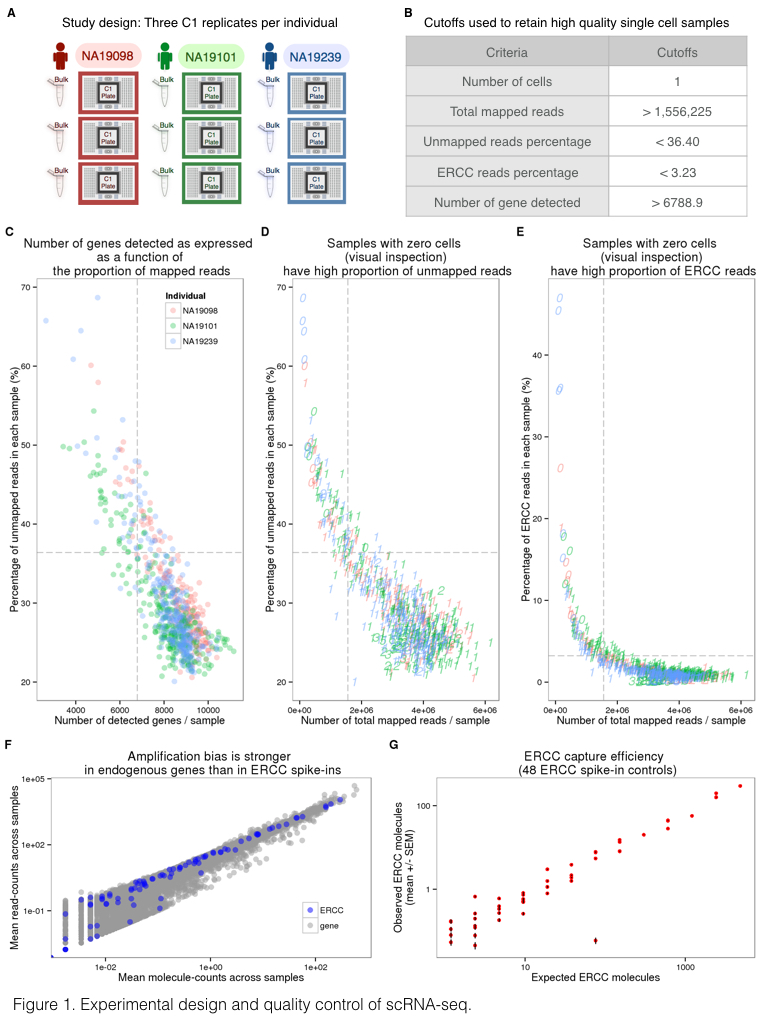
\includegraphics[trim=0 .5in 0 0,clip,width=5in]{img/ch04/Figure01.jpeg}
\caption[Experimental design and quality control of
scRNA-seq.]{\textbf{Experimental design and quality control of
scRNA-seq.} (A) Three C1 96 well-integrated fluidic circuit (IFC)
replicates were collected from each of the three Yoruba individuals. A
bulk sample was included in each batch. (B) Summary of the cutoffs used
to remove data from low quality cells that might be ruptured or dead
(See Supplementary Fig. \ref{fig:ch04-s1} for details). (C-E) To assess the quality of
the scRNA-seq data, the capture efficiency of cells and the faithfulness
of mRNA fraction amplification were determined based on the proportion
of unmapped reads, the number of detected genes, the numbers of total
mapped reads, and the proportion of ERCC spike-in reads across cells.
The dash lines indicate the cutoffs summarized in panel (B). The three
colors represent the three individuals (NA19098 in red, NA19101 in
green, and NA19239 in blue), and the numbers indicate the cell numbers
observed in each capture site on C1 plate.}
\label{fig:ch04-study-design}
\end{figure}

% Continues caption on next page. Requires package ccaption.
\begin{figure}
\contcaption{(continued) (F) Scatterplots in log scale
showing the mean read counts and the mean molecule counts of each
endogenous gene (grey) and ERCC spike-ins (blue) from the 564 high
quality single cell samples before removal of genes with low expression.
(G) mRNA capture efficiency shown as observed molecule count versus
number of molecules added to each sample, only including the 48 ERCC
spike-in controls remaining after removal of genes with low abundance.
Each red dot represents the mean +/- SEM of an ERCC spike-in across the
564 high quality single cell samples.}
\end{figure}

In what follows, we describe data as originating from different samples
when we refer to data from distinct wells of each C1 collection.
Generally, each sample corresponds to a single cell. In turn, we
describe data as originating from different replicates when we refer to
all samples from a given C1 collection, and from different individuals
when we refer to data from all samples and replicates of a given
genetically distinct iPSC line.

We obtained an average of 6.3 +/- 2.1 million sequencing reads per
sample (range 0.4-11.2 million reads). We processed the sequencing reads
using a standard alignment approach (see Methods) and performed multiple
quality control analyses. As a first step, we estimated the proportion
of ERCC spike-in reads from each sample. We found that, across samples,
sequencing reads from practically all samples of the second replicate of
individual NA19098 included unusually high ERCC content compared to all
other samples and replicates (Supplementary Fig. \ref{fig:ch04-s1}). We concluded that
a pipetting error led to excess ERCC content in this replicate and we
excluded the data from all samples of this replicate in subsequent
analyses. With the exception of the excluded samples, data from all
other replicates seem to have similar global properties (using general
metrics; Fig. \ref{fig:ch04-study-design}C-E and Supplementary Fig. \ref{fig:ch04-s1}).

We next examined the assumption that data from each sample correspond to
data from a single cell. After the cell sorting was complete, but before
the processing of the samples, we performed visual inspection of the C1
microfluidic plates. Based on that visual inspection, we flagged 21
samples that did not contain any cell, and 54 samples that contained
more than one cell (across all batches). Visual inspection of the C1
microfluidic plate is an important quality control step, but it is not
infallible. We therefore filtered data from the remaining samples based
on the number of total mapped reads, the percentage of unmapped reads,
the percentage of ERCC spike-in reads, and the number of genes detected
(Fig. \ref{fig:ch04-study-design}B-E). We chose data-driven inclusion cutoffs for each metric,
based on the 95th percentile of the respective distributions for the 21
libraries that were amplified from samples that did not include a cell
based on visual inspection (Supplementary Fig. \ref{fig:ch04-s1}). Using this approach,
we identified and removed data from 15 additional samples that were
classified as originating from a single cell based on visual inspection,
but whose data were more consistent with a multiple-cell origin based on
the number of total molecules, the concentration of cDNA amplicons, and
the read-to-molecule conversion efficiency (defined as the number of
total molecules divided by the number of total reads; Supplementary Fig.
\ref{fig:ch04-s2}). At the conclusion of these quality control analyses and exclusion
steps, we retained data from 564 high quality samples, which correspond,
with reasonable confidence, to 564 single cells, across eight replicates
from three individuals (Supplementary Table \ref{tab:ch04-s2}).

Our final quality check focused on the different properties of
sequencing read and molecule count data. We considered data from the 564
high quality samples and compared gene specific counts of sequencing
read and molecules. We found that while gene-specific reads and molecule
counts are exceptionally highly correlated when we considered the ERCC
spike-in data (r = 0.99; Fig. \ref{fig:ch04-study-design}F), these counts are somewhat less
correlated when data from the endogenous genes are considered (r =
0.92). Moreover, the gene-specific read and molecule counts correlation
is noticeably lower for genes that are expressed at lower levels (Fig.
1F). These observations concur with previous studies \citep{Islam2014,
Grun2014} as they underscore the importance of using UMIs in single
cell gene expression studies.

\begin{figure}
\centering
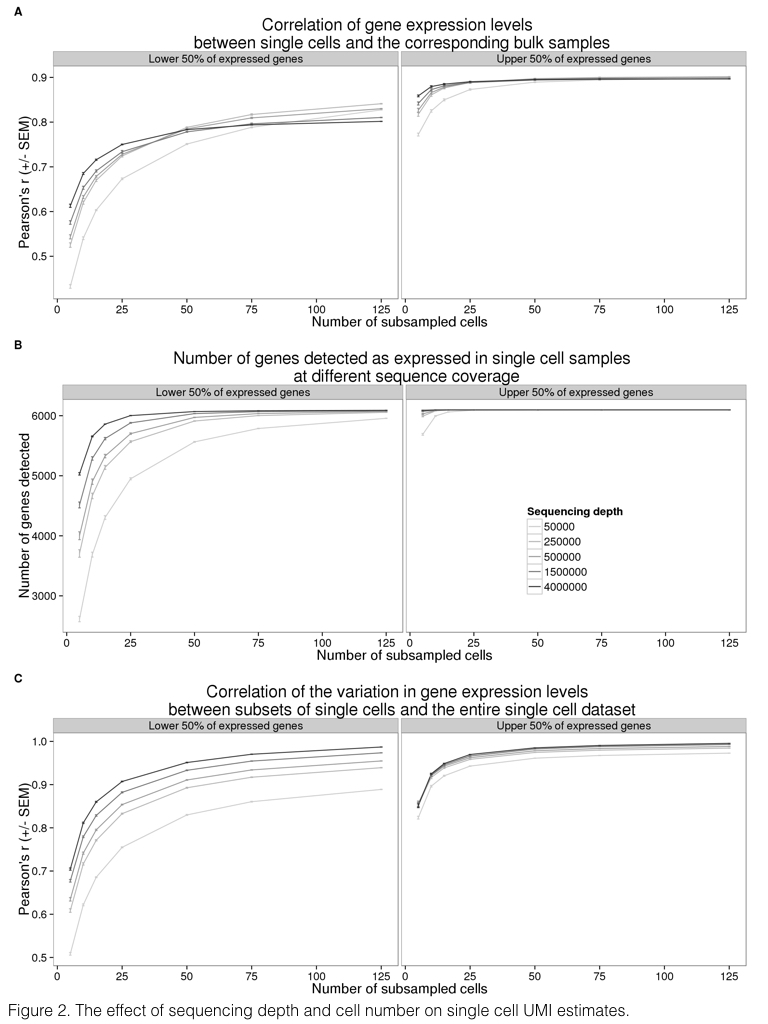
\includegraphics[trim=0 .3in 0 0,clip,width=5in]{img/ch04/Figure02.jpeg}
\caption[The effect of sequencing depth and cell
number on single cell UMI estimates.]{\textbf{The effect of sequencing depth and cell
number on single cell UMI estimates.} Sequencing reads from the entire
data set were subsampled to the indicated sequencing depth and cell
number, and subsequently converted to molecules using the UMIs. Each
point represents the mean +/- SEM of 10 random draws of the indicated
cell number. The left panel displays the results for 6,097 (50\% of
detected) genes with lower expression levels and the right panel the
results for 6,097 genes with higher expression levels. (A) Pearson
correlation of aggregated gene expression level estimates from single
cells compared to the bulk sequencing samples. (B) Total number of genes
detected with at least one molecule in at least one of the single cells.
(C) Pearson correlation of cell-to-cell gene expression variance
estimates from subsets of single cells compared to the full single cell
data set.}
\label{fig:subsample}
\end{figure}

We proceeded by investigating the effect of sequencing depth and the
number of single cells collected on multiple properties of the data. To
this end, we repeatedly subsampled single cells and sequencing reads to
assess the correlation of the single cell gene expression estimates to
the bulk samples, the number of genes detected, and the correlation of
the cell-to-cell gene expression variance estimates between the reduced
subsampled data and the full single cell gene expression data set (Fig.
2). We observed quickly diminishing improvement in all three properties
with increasing sequencing depth and the number of sampled cells,
especially for highly expressed genes. For example, a per cell
sequencing depth of 1.5 million reads (which corresponds to
\mytilde50,000 molecules) from each of 75 single cells was
sufficient for effectively quantifying even the lower 50\% of expressed
genes. To be precise, at this level of subsampling for individual NA19239, we were able
to detect a mean of 6068 genes out of 6097 genes expressed in the bulk
samples (the bottom 50\%; Fig. \ref{fig:subsample}B); the estimated single cell expression
levels of these genes (summed across all cells) correlated with the bulk
sample gene expression levels with a mean Pearson coefficient of 0.8
(Fig. \ref{fig:subsample}A), and the estimated cell-to-cell variation in gene expression
levels was correlated with the variation estimated from the full data
set with a mean Pearson coefficient of 0.95 (Fig. \ref{fig:subsample}C).

\subsection{Batch effects associated with UMI-based single cell
data}\label{batch-effects-associated-with-umi-based-single-cell-data}

In the context of the C1 platform, typical study designs make use of a
single C1 plate (batch/replicate) per biological condition. In that
case, it is impossible to distinguish between biological and technical
effects associated with the independent capturing and sequencing of each
C1 replicate. We designed our study with multiple technical replicates
per biological condition (individual) in order to directly and
explicitly estimate the batch effect associated with independent C1
preparations (Fig. \ref{fig:ch04-study-design}A).

As a first step in exploring batch effects, we examined the gene
expression profiles across all single cells that passed our quality
checks (as reported above) using raw molecule counts (without
standardization). Using principal component analysis (PCA) for
visualization, we observed -- as expected - that the major source of
variation in data from single cells is the individual origin of the
sample (Fig. \ref{fig:normalization}A). Specifically, we found that the proportion of variance
due to individual was larger (median: 8\%) than variance due to C1 batch
(median: 4\%; Kruskal-Wallis test; \emph{P} \textless{} 0.001,
Supplementary Fig. \ref{fig:ch04-s3}; see Methods for details of the variance component
analysis). Yet, variation due to C1 batch is also substantial - data
from single cell samples within a batch are more correlated than that
from single cells from the same individual but different batches
(Kruskal-Wallis test; \emph{P} \textless{} 0.001).

Could we account for the observed batch effects using the ERCC spike-in
controls? In theory, if the total ERCC molecule-counts are affected only
by technical variability, the spike-ins could be used to correct for
batch effects even in a study design that entirely confounds biological
samples with C1 preparations. To examine this, we first considered the
relationship between total ERCC molecule-counts and total endogenous
molecule-counts per sample. If only technical variability affects ERCC
molecule-counts, we expect the technical variation in the spike-ins
(namely, variation between C1 batches) to be consistent, regardless of
the individual assignment. Indeed, we observed that total ERCC
molecule-counts are significantly different between C1 batches (F-test;
\emph{P} \textless{} 0.001). However, total ERCC molecule-counts are
also quite different across individuals, when variation between batches
is taken into account (LRT; \emph{P} = 0.08; Fig. \ref{fig:batch}A). This observation
suggests that both technical and biological variation affect total ERCC
molecule-counts. In addition, while we observed a positive relationship
between total ERCC molecule-counts and total endogenous molecule-counts
per sample, this correlation pattern differed across C1 batches and
across individuals (F-test; \emph{P} \textless{} 0.001; Fig. \ref{fig:batch}B).

To more carefully examine the technical and biological variation of ERCC
spike-in controls, we assessed the ERCC per-gene expression profile. We
observed that the ERCC gene expression data from samples of the same
batch were more correlated than data from samples across batches
(Kruskal-Wallis test; Chi-squared \emph{P} \textless{} 0.001). However,
the proportion of variance explained by the individual was significantly
larger than the variance due to C1 batch (median: 9\% vs.~5\%,
Chi-squared test; \emph{P} \textless{} 0.001, Supplementary Fig. \ref{fig:ch04-s3}),
lending further support to the notion that biological variation affects
the ERCC spike in data. Based on these analyses, we concluded that ERCC
spike-in controls cannot be used to effectively account for the batch
effect associated with independent C1 preparations.

\begin{figure}
\centering
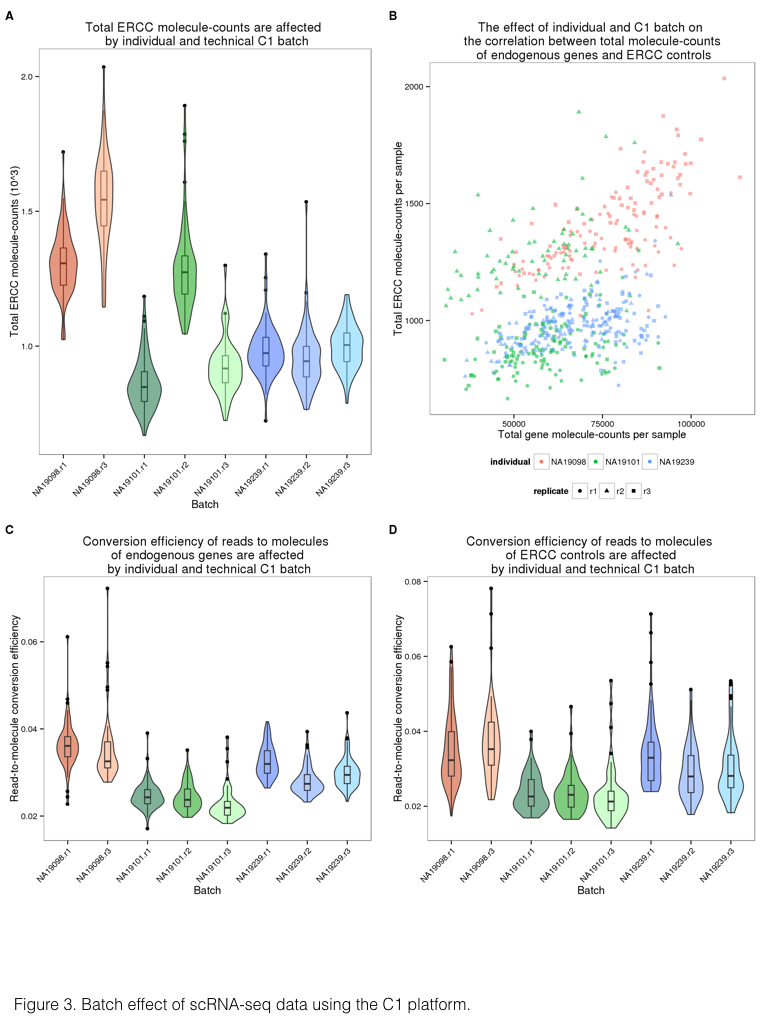
\includegraphics[trim=0 .5in 0 0,clip,width=5in]{img/ch04/Figure03.jpeg}
\caption[Batch effect of scRNA-seq data using the C1
platform.]{\textbf{Batch effect of scRNA-seq data using the C1
platform.} (A) Violin plots of the number of total ERCC spike-in
molecule-counts in single cell samples per C1 replicate. (B) Scatterplot
of the total ERCC molecule-counts and total gene molecule-counts. The
colors represent the three individuals (NA19098 is in red, NA19101 in
green, and NA19239 in blue). Data from different C1 replicates is
plotted in different shapes. (C and D) Violin plots of the reads to
molecule conversion efficiency (total molecule-counts divided by total
read-counts per single cells) by C1 replicate. The endogenous genes and
the ERCC spike-ins are shown separately in (C) and (D), respectively.
There is significant difference across individuals of both endogenous
genes (\emph{P} \textless{} 0.001) and ERCC spike-ins (\emph{P}
\textless{} 0.05). The differences across C1 replicates per individual
of endogenous genes and ERCC spike-ins were also evaluated (both
\emph{P} \textless{} 0.01).}
\label{fig:batch}
\end{figure}

We explored potential reasons for the observed batch effects, and in
particular, the difference in ERCC counts across batches and
individuals. We focused on the read-to-molecule conversion rates,
i.e.~the rates at which sequencing reads are converted to molecule
counts based on the UMI sequences. We defined read-to-molecule
conversion efficiency as the total molecule-counts divided by the total
reads-counts in each sample, considering separately the reads/molecules
that correspond to endogenous genes or ERCC spike-ins (Fig. \ref{fig:batch}C and \ref{fig:batch}D).
We observed a significant batch effect in the read-to-molecule
conversion efficiency of both ERCC (F-test; \emph{P} \textless{} 0.05)
and endogenous genes (F-test; \emph{P} \textless{} 0.001) across C1
replicates from the same individual. Moreover, the difference in
read-to-molecule conversion efficiency across the three individuals was
significant not only for endogenous genes (LRT; \emph{P} \textless{}
0.01, Fig. \ref{fig:batch}C) but also in the ERCC spike-ins (LRT; \emph{P} \textless{}
0.01, Fig. \ref{fig:batch}D). We reason that the difference in read to molecule
conversion efficiency across C1 preparations may contribute to the
observed batch effect in this platform.

\subsection{Measuring regulatory noise in single-cell gene expression
data}\label{measuring-regulatory-noise-in-single-cell-gene-expression-data}

Our analysis indicated that there is a considerable batch effect in the
single cell gene expression data collected from the C1 platform. We thus
sought an approach that would account for the batch effect and allow us
to study biological properties of the single-cell molecule count-based
estimates of gene expression levels, albeit in a small sample of just
three individuals. As a first step, we adjusted the raw molecule counts
by using a Poisson approximation to account for the random use of
identical UMI sequences in molecules from highly expressed genes (this
was previously termed a correction for the UMI `collision probability'
\citep{Fu2011}). We then excluded data from genes whose inferred molecule
count exceeded 1,024 (the theoretical number of UMI sequences) -- this
step resulted in the exclusion of data from 6 mitochondrial genes.

\begin{figure}
\centering
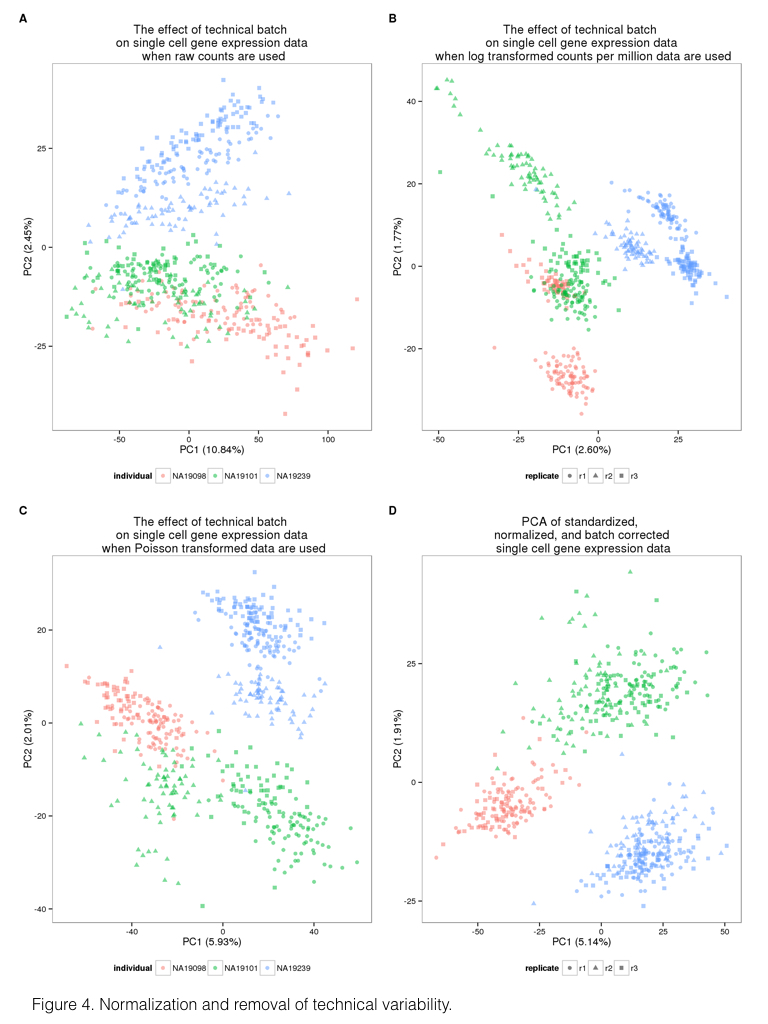
\includegraphics[trim=0 .5in 0 0,clip,width=5in]{img/ch04/Figure04.jpeg}
\caption[Normalization and removal of technical
variability.]{\textbf{Normalization and removal of technical
variability.} Principal component (PC) 1 versus PC2 of the (A) raw
molecule counts, (B) log\textsubscript{2} counts per million (cpm), (C)
Poisson transformed expression levels (accounting for technical
variability modeled by the ERCC spike-ins), and (D) batch-corrected
expression levels. The colors represent the three individuals (NA19098
in red, NA19101 in green, and NA19239 in blue). Data from different C1
replicates is plotted in different shapes.}
\label{fig:normalization}
\end{figure}

We next incorporated a standardization step by computing log transformed
counts-per-million (cpm) to remove the effect of different sequencing
depths, as is the common practice for the analysis of bulk RNA-seq data
(Fig. \ref{fig:normalization}A and \ref{fig:normalization}B). We used a Poisson generalized linear model to
normalize the endogenous molecule log\textsubscript{2} cpm values by the
observed molecule counts of ERCC spike-ins across samples. While we do
not expect this step to account for the batch effect (as discussed
above), we reasoned that the spike-ins allow us to account for a subset
of technical differences between samples, for example, those that arise
from differences in RNA concentration (Fig. \ref{fig:normalization}C).

Finally, to account for the technical batch effect, we modeled
between-sample correlations in gene expression within C1 replicates (see
Methods). Our approach is similar in principle to limma, which was
initially developed for adjusting within-replicate correlations in
microarray data \citep{Smyth2005}. We assume that samples within each C1
replicate share a component of technical variation, which is independent
of biological variation across individuals. We fit a linear mixed model
for each gene, which includes a fixed effect for individual and a random
effect for batch. The batch effect is specific to each C1 replicate, and
is independent of biological variation across individuals. We use this
approach to estimate and remove the batch effect associated with
different C1 preparations (Fig. \ref{fig:normalization}D).

Once we removed the unwanted technical variability, we focused on
analyzing biological variation in gene expression between single cells.
Our goal was to identify inter-individual differences in the amount of
variation in gene expression levels across single cells, or in other
words, to identify differences between individuals in the amount of
regulatory noise \citep{Raser2005}. In this context, regulatory noise is
generally defined as the coefficient of variation (CV) of the gene
expression levels of single cells \citep{Fehrmann2013}. In the following,
we used the standardized, normalized, batch-corrected molecule count
gene expression data to estimate regulatory noise (Fig. \ref{fig:normalization}D). To account
for heteroscedasticity from Poisson sampling, we adjusted the CV values
by the average gene-specific expression level across cells of the same
individual. The adjusted CV is robust both to differences in gene
expression levels, as well as to the proportion of gene dropouts in
single cells.

To investigate the effects of gene dropouts (the lack of molecule
representation of an expressed gene \citep{Brennecke2013, Shalek2013})
on our estimates of gene expression noise, we considered the association
between the proportion of cells in which a given gene is undetected
(namely, the gene-specific dropout rate), the average gene expression
level, and estimates of gene expression noise. Across all genes, the
median gene-specific dropout was 22 percent. We found significant
individual differences (LRT; \emph{P} \textless{}
10\textsuperscript{-5}) in gene-specific dropout rates between
individuals in more than 10\% (1,214 of 13,058) of expressed endogenous
genes. As expected, the expression levels, and the estimated variation
in expression levels across cells, are both associated with
gene-specific dropout rates (Supplementary Fig. \ref{fig:ch04-s4}). However,
importantly, adjusted CVs are not associated with dropout rates
(Spearman's correlation = 0.04; Supplementary Fig. \ref{fig:ch04-s4}), indicating that
adjusted CV measurements are not confounded by the dynamic range of
single-cell gene expression levels.

We thus estimated mean expression levels and regulatory noise (using
adjusted CV) for each gene, by either including (Fig. \ref{fig:variation}A) or excluding
(Fig. \ref{fig:variation}B) samples in which the gene was not detected/expressed. We first
focused on general trends in the data. We ranked genes in each
individual by their mean expression level as well as by their estimated
level of variation across single cells. When we considered samples in
which a gene was expressed, we found that 887 of the 1,000 most highly
expressed genes in each individual are common to all three individuals
(Fig. \ref{fig:variation}C). In contrast, only 103 of the 1,000 most highly variable
(noisy) genes in each individual were common to all three individuals
(Fig. \ref{fig:variation}D). We found similar results when we considered data from all
single cells, regardless of whether the gene was detected as expressed
(Fig. \ref{fig:variation}E and \ref{fig:variation}F).

Next, we identified genes whose estimated regulatory noise (based on the
adjusted CV) is significantly different between individuals. For the
purpose of this analysis, we only included data from cells in which the
gene was detected as expressed. Based on permutations (Supplementary
Fig. \ref{fig:ch04-s5}), we classified the estimates of regulatory noise of 560 genes
as significantly different across individuals (empirical \emph{P}
\textless{} .0001, Supplementary Fig. \ref{fig:ch04-s6} for examples; Supplementary
Table \ref{tab:ch04-s3} for gene list). These 560 genes are enriched for genes involved
in protein translation, protein disassembly, and various biosynthetic
processes (Supplementary Table \ref{tab:ch04-s4}). Interestingly, among the genes whose
regulatory noise estimates differ between individuals, we found two
pluripotency genes, \emph{KLF4} and \emph{DPPA2} (Supplementary Fig.
\ref{fig:ch04-s7}).

\begin{figure}
\centering
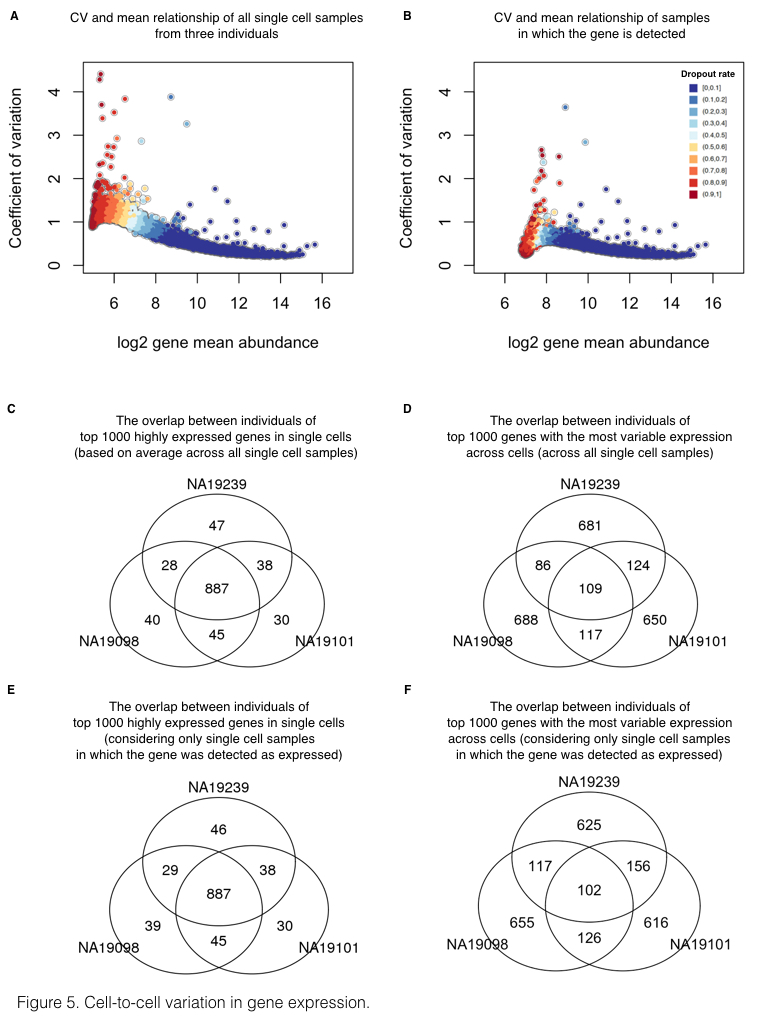
\includegraphics[trim=0 .5in 0 0,clip,width=5in]{img/ch04/Figure05.jpeg}
\caption[Cell-to-cell variation in gene expression.]{\textbf{Cell-to-cell variation in gene expression.}
Adjusted CV plotted against average molecule counts across all cells in
(A) and across only the cells in which the gene is expressed (B),
including data from all three individuals. Each dot represents a gene,
and the color indicates the corresponding gene-specific dropout rate
(the proportion of cells in which the gene is undetected). (C and D)
Venn diagrams showing the overlaps of top 1000 genes across individuals
based on mean expression level in (C) and based on adjusted CV values in
(D), considering only the cells in which the gene is expressed. (E and
F) Similarly, Venn diagrams showing the overlaps of top 1000 genes
across individuals based on mean expression level in (E) and based on
adjusted CV values in (F), across all cells.}
\label{fig:variation}
\end{figure}

\section{Discussion}\label{ch04-discussion}

\subsection{Study design and sample size for
scRNA-seq}\label{study-design-and-sample-size-for-scrna-seq}

Our nested study design allowed us to explicitly estimate technical
batch effects associated with single cell sample processing on the C1
platform. We found previously unreported technical sources of variation
associated with the C1 sample processing and the use of UMIs, including
the property of batch-specific read-to-molecule conversion efficiency.
As we used a well-replicated nested study design, we were able to model,
estimate, and account for the batch while maintaining individual
differences in gene expression levels. We believe that our observations
indicate that future studies should avoid confounding C1 batch and
individual source of single cell samples. Instead, we recommend a
balanced study design consisting of multiple individuals within a C1
plate and multiple C1 replicates (for example, Supplementary Fig. \ref{fig:ch04-s8}).
The origin of each cell can then be identified using the RNA sequencing
data. Indeed, using a method originally developed for detecting sample
swaps in DNA sequencing experiments \citep{Jun2012}, we were able to
correctly identify the correct YRI individual of origin for all the
single cells from the current experiment by comparing the polymorphisms
identified using the RNA-seq reads to the known genotypes for all 120
YRI individuals of the International HapMap Project
\citep{HapMapConsortium2005} (Supplementary Fig. \ref{fig:ch04-s8}). The
mixed-individual-plate is an attractive study design because it allows
one to account for the batch effect without the requirement to
explicitly spend additional resources on purely technical replication
(because the total number of cells assayed from each individual can be
equal to a design in which one individual is being processed in using a
single C1 plate).

We also addressed additional study design properties with respect to the
desired number of single cells and the desired depth of sequencing (Fig.
2). Similar assessments have been previously performed for single cell
sequencing with the C1 platform without the use of UMIs \citep{Wu2014,
Pollen2014}, but no previous study has investigated the effects of
these parameters for single cells studies using UMIs. We focused on
recapitulating the gene expression levels observed in bulk sequencing
experiments, detecting as many genes as possible, and accurately
measuring the cell-to-cell variation in gene expression levels. We
recommend sequencing at least 75 high quality cells per biological
condition with a minimum of 1.5 million raw reads per cell to obtain
optimal performance of these three metrics.

\subsection{The limitations of the ERCC spike-in
controls}\label{the-limitations-of-the-ercc-spike-in-controls}

The ERCC spike-in controls have been used in previous scRNA-seq studies
to identify low quality single cell samples, infer the absolute total
number of molecules per cell, and model the technical variability across
cells \citep{Brennecke2013, Grun2014, Ding2015, Vallejos2015}. In our
experience, the ERCC controls are not particularly well-suited for any
one of these tasks, much less all three. With respect to identifying low
quality samples, we indeed observed that samples with no visible cell
had a higher percentage of reads mapping to the ERCC controls, as
expected. However, there was no clear difference between low and high
quality samples in the percentage of ERCC reads or molecules, and thus
any arbitrarily chosen cutoff would be associated with considerable
error (Fig. \ref{fig:ch04-study-design}E). With respect to inferring the absolute total number of
molecules per cell, we observed that the biological covariate of
interest (difference between the three YRI individuals), rather than
batch, explained a large proportion of the variance in the ERCC counts
(Supplementary Fig. \ref{fig:ch04-s3}), and furthermore that the ERCC controls were
also affected by the individual-specific effect on the read-to-molecule
conversion rate (Fig. \ref{fig:batch}D). Thus ERCC-based corrected estimates of total
number of molecules per cell, across technical or biological replicates,
are expected to be biased. Because the batch effects associated with the
ERCC controls are driven by the biological covariate of interest, they
will also impede the modeling of the technical variation in single cell
experiments that confound batch and the biological source of the single
cells.

More generally, it is inherently difficult to model unknown sources of
technical variation using so few genes \citep{Risso2014} (only
approximately half of the 92 ERCC controls are detected in typical
single cell experiments), and the ERCC controls are also strongly
impacted by technical sources of variation even in bulk RNA-seq
experiments \citep{SEQC/MAQC-IIIConsortium2014}. Lastly, from a
theoretical perspective, the ERCC controls have shorter polyA tails and
are overall shorter than mammalian mRNAs. For these reasons, we caution
against the reliance of ERCC controls in scRNA-seq studies and highlight
that an alternative set of controls that more faithfully mimics
mammalian mRNAs and provides more detectable spike-in genes is desired.
Our recommendation is to include total RNA from a distant species, for
example using RNA from \emph{Drosophila} \emph{melanogaster} in studies
of single cells from humans.

\subsection{Outlook}\label{outlook}

Single cell experiments are ideally suited to study gene regulatory
noise and robustness \citep{Borel2015, Finak2015}. Yet, in order to
study the biological noise in gene expression levels, it is imperative
that one should be able to effectively estimate and account for the
technical noise in single cell gene expression data. Our results
indicate that previous single cells gene expression studies may not have
been able to distinguish between the technical and the biological
components of variation, because single cell samples from each
biological condition were processed on a single C1 batch. When technical
noise is properly accounted for, even in this small pilot study, our
findings indicate pervasive inter-individual differences in gene
regulatory noise, independently of the overall gene expression level.

\section{Methods}\label{ch04-methods}

\subsection{Ethics statement}\label{ch04-ethics-statement}

The YRI cell lines were purchased from CCR. The original samples were
collected by the HapMap project between 2001-2005. All of the samples
were collected with extensive community engagement, including
discussions with members of the donor communities about the ethical and
social implications of human genetic variation research. Donors gave
broad consent to future uses of the samples, including their use for
extensive genotyping and sequencing, gene expression and proteomics
studies, and all other types of genetic variation research, with the
data publicly released.

\subsection{Cell culture of iPSCs}\label{cell-culture-of-ipscs}

Undifferentiated feeder-free iPSCs reprogrammed from LCLs of Yoruba
individuals in Ibadan, Nigeria (abbreviation: YRI)
\citep{HapMapConsortium2005} were grown in E8 medium (Life Technologies)
\citep{Chen2011} on Matrigel-coated tissue culture plates with daily
media feeding at 37 °C with 5\% (vol/vol) CO2. For standard maintenance,
cells were split every 3-4 days using cell release solution (0.5 mM EDTA
and NaCl in PBS) at the confluence of roughly 80\%. For the single cell
suspension, iPSCs were individualized by Accutase Cell Detachment
Solution (BD) for 5-7 minutes at 37 °C and washed twice with E8 media
immediately before each experiment. Cell viability and cell counts were
then measured by the Automated Cell Counter (Bio-Rad) to generate
resuspension densities of 2.5 X 105 cells/mL in E8 medium for C1 cell
capture.

\subsection{Single cell capture and library
preparation}\label{single-cell-capture-and-library-preparation}

Single cell loading and capture were performed following the Fluidigm
protocol (PN 100-7168). Briefly, 30 $\mu$l of C1 Suspension Reagent was
added to a 70-$\mu$l aliquot of \mytilde17,500 cells. Five
$\mu$l of this cell mix were loaded onto 10-17 $\mu$m C1 Single-Cell
Auto Prep IFC microfluidic chip (Fluidigm), and the chip was then
processed on a C1 instrument using the cell-loading script according to
the manufacturer's instructions. Using the standard staining script, the
iPSCs were stained with StainAlive TRA-1-60 Antibody (Stemgent, PN
09-0068). The capture efficiency and TRA-1-60 staining were then
inspected using the EVOS FL Cell Imaging System (Thermo Fisher)
(Supplementary Table \ref{tab:ch04-s1}).

Immediately after imaging, reverse transcription and cDNA amplification
were performed in the C1 system using the SMARTer PCR cDNA Synthesis kit
(Clontech) and the Advantage 2 PCR kit (Clontech) according to the
instructions in the Fluidigm user manual with minor changes to
incorporate UMI labeling \citep{Islam2014}. Specifically, the reverse
transcription primer and the 1:50,000 Ambion® ERCC Spike-In Mix1 (Life
Technologies) were added to the lysis buffer, and the template-switching
RNA oligos which contain the UMI (5-bp random sequence) were included in
the reverse transcription mix \citep{Islam2011, Islam2012, Islam2014}.
When the run finished, full-length, amplified, single-cell cDNA
libraries were harvested in a total of approximately 13 $\mu$l C1
Harvesting Reagent and quantified using the DNA High Sensitivity LabChip
(Caliper). The average yield of samples per C1 plate ranged from
1.26-1.88 ng per microliter (Supplementary Table \ref{tab:ch04-s1}). A bulk sample, a
40 $\mu$l aliquot of \mytilde10,000 cells, was collected in
parallel with each C1 chip using the same reaction mixes following the
C1 protocol (PN 100-7168, Appendix A).

For sequencing library preparation, tagmentation and isolation of 5'
fragments were performed according to the UMI protocol \citep{Islam2014}.
Instead of using commercially available Tn5 transposase, Tn5 protein
stock was freshly purified in house using the IMPACT system (pTXB1, NEB)
following the protocol previously described \citep{Picelli2014}. The
activity of Tn5 was tested and shown to be comparable with the
EZ-Tn5-Transposase (Epicentre). Importantly, all the libraries in this
study were generated using the same batch of Tn5 protein purification.
For each of the bulk samples, two libraries were generated using two
different indices in order to get sufficient material for sequencing.
All 18 bulk libraries were then pooled and labeled as the ``bulk'' for
sequencing.

\subsection{Illumina high-throughput
sequencing}\label{illumina-high-throughput-sequencing}

The scRNA-seq libraries generated from the 96 single cell samples of
each C1 chip were pooled and then sequenced in three lanes on an
Illumina HiSeq 2500 instrument using the PCR primer (C1-P1-PCR-2:
Bio-GAATGATACGGCGACCACCGAT) as the read 1 primer and the Tn5 adapter
(C1-Tn5-U: PHO-CTGTCTCTTATACACATCTGACGC) as the index read primer
following the UMI protocol \citep{Islam2014}.

The master mixes, one mix with all the bulk samples and nine mixes
corresponding to the three replicates for the three individuals, were
sequenced across four flowcells using a design aimed to minimize the
introduction of technical batch effects (Supplementary Table \ref{tab:ch04-s1}).
Single-end 100 bp reads were generated along with 8-bp index reads
corresponding to the cell-specific barcodes. We did not observe any
obvious technical effects due to sequencing lane or flow cell that
confounded the inter-individual and inter-replicate comparisons.

\subsection{Read mapping}\label{read-mapping}

To assess read quality, we ran FastQC
(\url{http://www.bioinformatics.babraham.ac.uk/projects/fastqc}) and
observed a decrease in base quality at the 3' end of the reads. Thus we
removed low quality bases from the 3' end using sickle with default
settings \citep{Joshi2011}. To handle the UMI sequences at the 5' end of
each read, we used umitools \citep{umitools} to find all reads with a UMI
of the pattern NNNNNGGG (reads without UMIs were discarded). We then
mapped reads to human genome hg19 (only including chromosomes 1-22, X,
and Y, plus the ERCC sequences) with Subjunc \citep{Liao2013}, discarding
non-uniquely mapped reads (option -u). To obtain gene-level counts, we
assigned reads to protein-coding genes (Ensembl GRCh37 release 82) and
the ERCC spike-in genes using featureCounts \citep{Liao2014}. Because the
UMI protocol maintains strand information, we required that reads map to
a gene in the correct orientation (featureCounts flag -s 1).

In addition to read counts, we utilized the UMI information to obtain
molecule counts for the single cell samples. We did not count molecules
for the bulk samples because this would violate the assumptions of the
UMI protocol, as bulk samples contain far too many unique molecules for
the 1,024 UMIs to properly tag them all. First, we combined all reads
for a given single cell using samtools \citep{Li2009}. Next, we converted
read counts to molecule counts using UMI-tools \citep{Smith2016}.
UMI-tools counts the number of UMIs at each read start position.
Furthermore, it accounts for sequencing errors in the UMIs introduced
during the PCR amplification or sequencing steps using a ``directional
adjacency'' method. Briefly, all UMIs at a given read start position are
connected in a network using an edit distance of one base pair. However,
edges between nodes (the UMIs) are only formed if the nodes have less
than a 2x difference in reads. The node with the highest number of reads
is counted as a unique molecule, and then it and all connected nodes are
removed from the network. This is repeated until all nodes have been
counted or removed.

\subsection{Filtering cells and
genes}\label{filtering-cells-and-genes}

We performed multiple quality control analyses to detect and remove data
from low quality cells. In an initial analysis investigating the
percentage of reads mapping to the ERCC spike-in controls, we observed
that replicate 2 of individual NA19098 was a clear outlier
(Supplementary Fig. \ref{fig:ch04-s1}). It appeared that too much ERCC spike-in mix was
added to this batch, which violated the assumption that the same amount
of ERCC molecules was added to each cell. Thus, we removed this batch
from all of our analyses.

Next, we kept data from high quality single cells that passed the
following criteria:

\begin{itemize}
\itemsep1pt\parskip0pt\parsep0pt
\item
  Only one cell observed per well
\item
  At least 1,556,255 mapped reads
\item
  Less than 36.4\% unmapped reads
\item
  Less than 3.2\% ERCC reads
\item
  More than 6,788 genes with at least one read
\end{itemize}

We chose the above criteria based on the distribution of these metrics
in the empty wells (the cutoff is the 95th percentile, Supplementary
Fig. \ref{fig:ch04-s1}). In addition, we observed that some wells classified as
containing only one cell were clustered with multi-cell wells when
plotting 1) the number of gene molecules versus the concentration of the
samples, and 2) the read to molecule conversion efficiency (total
molecule number divided by total read number) of endogenous genes versus
that of ERCC. We therefore established filtering criteria for these
misidentified single-cell wells using linear discriminant analysis
(LDA). Specifically, LDA was performed to classify wells into empty,
one-cell, and two-cell using the discriminant functions of 1) sample
concentration and the number of gene molecules, and 2) endogenous and
ERCC gene read to molecule conversion efficiency (Supplementary Fig.
\ref{fig:ch04-s2}). After filtering, we maintained 564 high quality single cells
(NA19098: 142, NA19101: 201, NA19239: 221).

The quality control analyses were performed using all protein-coding
genes (Ensembl GRCh37 release 82) with at least one observed read. Using
the high quality single cells, we further removed genes with low
expression levels for downstream analyses. We removed all genes with a
mean log\textsubscript{2} cpm less than 2, which did not affect the
relative differences in the proportion of genes detected across batches
(Supplementary Fig. \ref{fig:ch04-s9}). We also removed genes with molecule counts
larger than 1,024 for the correction of collision probability. In the
end we kept 13,058 endogenous genes and 48 ERCC spike-in genes.

\subsection{Calculate the input molecule quantities of ERCC
spiked-ins}\label{calculate-the-input-molecule-quantities-of-ercc-spiked-ins}

According to the information provided by Fluidigm, each of the 96
capture chamber received 13.5 nl of lysis buffer, which contain 1:50,000
Ambion® ERCC Spike-In Mix1 (Life Technologies) in our setup. Therefore,
our estimation of the total spiked-in molecule number was 16,831 per
sample. Since the relative concentrations of the ERCC genes were
provided by the manufacturer, we were able to calculate the molecule
number of each ERCC gene added to each sample. We observed that the
levels of ERCC spike-ins strongly correlated with the input quantities
(r = 0.9914, Fig. \ref{fig:ch04-study-design}G). The capture efficiency, defined as the fraction
of total input molecules being successfully detected in each high
quality cell, had an average of 6.1\%.

\subsection{Subsampling}\label{subsampling}

We simulated different sequencing depths by randomly subsampling reads
and processing the subsampled data through the same pipeline described
above to obtain the number of molecules per gene for each single cell.
To assess the impact of sequencing depth and number of single cells, we
calculated the following three statistics:

\begin{enumerate}
\def\labelenumi{\arabic{enumi}.}
\itemsep1pt\parskip0pt\parsep0pt
\item
  The Pearson correlation of the gene expression level estimates from
  the single cells compared to the bulk samples. For the single cells,
  we summed the gene counts across all the samples and then calculated
  the log\textsubscript{2} cpm of this pseudo-bulk. For the bulk
  samples, we calculated the log\textsubscript{2} cpm separately for
  each of the three replicates and then calculated the mean per gene.
\item
  The number of genes detected with at least one molecule in at least
  one cell.
\item
  The Pearson correlation of the cell-to-cell gene expression variance
  estimates from the subsampled single cells compared to the variance
  estimates using the full single cell data set.
\end{enumerate}

Each data point in Fig. \ref{fig:subsample} represents the mean +/- the standard error of
the mean (SEM) of 10 random subsamples of cells. We split the genes by
expression level into two groups (6,097 genes each) to highlight that
most of the improvement with increased sequencing depth and number of
cells was driven by the estimates of the lower half of expressed genes.
The data shown is for individual NA19239, but the results were
consistent for individuals NA19098 and NA19101. Only high quality single
cells (Supplementary Table \ref{tab:ch04-s2}) were included in this analysis.

\subsection{A framework for testing individual and batch
effects}\label{a-framework-for-testing-individual-and-batch-effects}

Individual effect and batch effect between the single cell samples were
evaluated in a series of analyses that examine the potential sources of
technical variation on gene expression measurements. These analyses took
into consideration that in our study design, sources of variation
between single cell samples naturally fall into a hierarchy of
individuals and C1 batches. In these sample-level analyses, the
variation introduced at both the individual-level and the batch-level
was modeled in a nested framework that allows random noise between C1
batches within individuals. Specifically, for each cell sample in
individual $i$, replicate $j$ and well $k$, we used $y_{ijk}$ to denote
some sample measurement (e.g.~total molecule-counts) and fit a linear
mixed model with the fixed effect of individual $\alpha_i$ and the
random effect of batch $b_{ij}$:

\[y_{ijk} = \alpha_{i} + b_{ij} + \epsilon_{ijk} \,\,\,\,(1)\]

where the random effect $b_{ij}$ of batch follows a normal distribution
with mean zero and variance $\sigma^2_{b}$, and $\epsilon_{ijk}$
describes residual variation in the sample measurement. To test the
statistical significance of individual effect (i.e., null hypothesis
$\alpha_1 = \alpha_2 = \alpha_3$), we performed a likelihood ratio test
(LRT) to compare the above full model and the reduced model that
excludes $\alpha_i$. To test if there was a batch effect (i.e., null
hypothesis $\sigma^2_b = 0$), we performed an F-test to compare the
variance that is explained by the above full model and the variance due
to the reduced model that excludes $b_{ij}$.

The nested framework was applied to test the individual and batch
effects between samples in the following cases. The data includes
samples after quality control and filtering.

\begin{enumerate}
\def\labelenumi{\arabic{enumi}.}
\item
  Total molecule count (on the log\textsubscript{2} scale) was modeled
  as a function of individual effect and batch effect, separately for
  the ERCC spike-ins and for the endogenous genes.
\item
  Read-to-molecule conversion efficiency was modeled as a function of
  individual effect and batch effect, separately for the ERCC spike-ins
  and for the endogenous genes.
\end{enumerate}

\subsection{Estimating variance components for per-gene expression
levels}\label{estimating-variance-components-for-per-gene-expression-levels}

To assess the relative contributions of individual and technical
variation, we analyzed per-gene expression profiles and computed
variance component estimates for the effects of individual and C1 batch
(Supplementary Fig. \ref{fig:ch04-s3}). The goal here was to quantify the proportion of
cell-to-cell variance due to individual (biological) effect and to C1
batch (technical) at the per-gene level. Note that the goal here was
different from that of the previous section, where we simply tested for
the existence of individual and batch effects at the sample level by
rejecting the null hypothesis of no such effects. In contrast, here we
fit a linear mixed model per gene where the dependent variable was the
gene expression level (log\textsubscript{2} counts per million) and the
independent variables were individual and batch, both modeled as random
effects.

The variance parameters of individual effect and batch effect were
estimated using a maximum penalized likelihood approach
\citep{Chung2013}, which can effectively avoid the common issue of zero
variance estimates due to small sample sizes (there were three
individuals and eight batches). We used the blmer function in the R
package blme and set the penalty function to be the logarithm of a gamma
density with shape parameter = 2 and rate parameter tending to zero.

The estimated variance components were used to compute the sum of
squared deviations for individual and batch effects. The proportion of
variance due to each effect is equal to the relative contribution of the
sum of squared deviations for each effect compared to the total sum of
squared deviations per gene. Finally, we compared the estimated
proportions of variance due to the individual effect and the batch
effect, across genes, using a non-parametric one-way analysis of
variance (Kruskal-Wallis rank sum test).

\subsection{Normalization}\label{normalization}

We transformed the single cell molecule counts in multiple steps (Fig.
4). First, we corrected for the collision probability using a method
similar to that developed by Grün et al. \citep{Grun2014}. Essentially we
corrected for the fact that we did not observe all the molecules
originally in the cell. The main difference between our approach and
that of Grün et al. \citep{Grun2014} was that we applied the correction
at the level of gene counts and not individual molecule counts. Second,
we standardized the molecule counts to log\textsubscript{2} counts per
million (cpm). This standardization was performed using only the
endogenous gene molecules and not the ERCC molecules. Third, we
corrected for cell-to-cell technical noise using the ERCC spike-in
controls. For each single cell, we fit a Poisson generalized linear
model (GLM) with the log\textsubscript{2} expected ERCC molecule counts
as the independent variable, and the observed ERCC molecule counts as
the dependent variable, using the standard log link function. Next we
used the slope and intercept of the Poisson GLM regression line to
transform the log\textsubscript{2} cpm for the endogenous genes in that
cell. This is analogous to the standard curves used for qPCR
measurements, but taking into account that lower concentration ERCC
genes will have higher variance from Poisson sampling. Fourth, we
removed technical noise between the eight batches (three replicates each
for NA19101 and NA19239 and two replicates for NA19098). We fit a linear
mixed model with a fixed effect for individual and a random effect for
the eight batches and removed the variation captured by the random
effect (see the next section for a detailed explanation).

For the bulk samples, we used read counts even though the reads
contained UMIs. Because these samples contained RNA molecules from
\mytilde10,000 cells, we could not assume that the 1,024 UMIs
were sufficient for tagging such a large number of molecules. We
standardized the read counts to log\textsubscript{2} cpm.

\subsection{Removal of technical batch
effects}\label{removal-of-technical-batch-effects}

Our last normalization step adjusted the transformed
log\textsubscript{2} gene expression levels for cell-to-cell correlation
within each C1 plate. The algorithm mimics a method that was initially
developed for adjusting within-replicate correlation in microarray data
\citep{Smyth2005}. We assumed that for each gene $g$, cells that belong
to the same batch $j$ are correlated, for batches $j = 1, \dots, 8$. The
batch effect is specific to each C1 plate and is independent of
biological variation across individuals.

We fit a linear mixed model for each gene $g$ that includes a fixed
effect of individual and a random effect for within-batch variation
attributed to cell-to-cell correlation in each C1 plate:

\[ y_{g,ijk} = \mu_{g} + \alpha_{g,i} + b_{g,ij} + \epsilon_{g,ijk}, \,\,\,\,(2)\]

where $y_{g,ijk}$ denotes log\textsubscript{2} counts-per-million (cpm)
of gene $g$ in individual $i$, replicate $j$, and cell $k$;
$i = NA19098, NA19101, NA19239$, $j = 1, \dots, n_i$ with $n_i$ the
number of replicates in individual $i$, $k = 1, \dots, n_{ij}$ with
$n_{ij}$ the number of cells in individual $i$ replicate $j$. $\mu_g$
denotes the mean gene expression level across cells, $\alpha_{g,i}$
quantifies the individual effect on mean gene expression, $b_{g,ij}$
models the replicate effect on mean expression level (assumed to be
stochastic, independent, and identically distributed with mean 0 and
variance $\sigma^2_{g,b}$). Finally, $\epsilon_{g,ijk}$ describes the
residual variation in gene expression.

Batch-corrected expression levels were computed as

\[ \widehat{y}_{g,ijk} = y_{g,ijk} - \widehat{b}_{g,ij}, \,\,\,\,(3)\]

where $\widehat{b}_{g,ij}$ are the least-squares estimates. The
computations in this step were done with the gls.series function of the
limma package \citep{Ritchie2015}.

\subsection{Measurement of gene expression
noise}\label{measurement-of-gene-expression-noise}

While examining gene expression noise (using the coefficient of
variation or CV) as a function of mean RNA abundance across C1
replicates, we found that the CV of molecule counts among endogenous
genes and ERCC spike-in controls suggested similar expression
variability patterns. Both endogenous and ERCC spike-in control CV
patterns approximately followed an over-dispersed Poisson distribution
(Supplementary Fig. \ref{fig:ch04-s10}), which is consistent with previous studies
\citep{Islam2014, Brennecke2013}. We computed a measure of gene
expression noise that is independent of RNA abundance across individuals
\citep{Kolodziejczyk2015, Newman2006}. First, squared coefficients of
variation (CVs) for each gene were computed for each individual and also
across individuals, using the batch-corrected molecule data. Then we
computed the distance of individual-specific CVs to the rolling median
of global CVs among genes that have similar RNA abundance levels. These
transformed individual CV values were used as our measure of gene
expression noise. Specifically, we computed the adjusted CV values as
follows:

\begin{enumerate}
\def\labelenumi{\arabic{enumi}.}
\item
  Compute squared CVs of molecule counts in each individual and across
  individuals.
\item
  Order genes by the global average molecule counts.
\item
  Starting from the genes with the lowest global average gene expression
  level, for every sliding window of 50 genes, subtract
  log\textsubscript{10} median squared CVs from log\textsubscript{10}
  squared CVs of each cell line, and set 25 overlapping genes between
  windows. The computation was performed with the rollapply function of
  the R zoo package \citep{Zeileis2005}. After this transformation step,
  CV no longer had a polynomial relationship with mean gene molecule
  count (Supplementary Fig. \ref{fig:ch04-s10}).
\end{enumerate}

\subsection{Identification of genes associated with inter-individual
differences in regulatory
noise}\label{identification-of-genes-associated-with-inter-individual-differences-in-regulatory-noise}

To identify differential noise genes across individuals, we computed
median absolute deviation (MAD) - a robust and distribution-free
dissimilarity measure for gene $g$:

\[ MAD_{g} = Median_{i= 1,2,3} \left| \text{adjCV}_{g,i} -  Median_{i= 1,2,3} ({\text{adjCV}}_{g,i}) \right|. \,\,\,\,(4)\]

Large values of $MAD_{g}$ suggest a large deviation from the median of
the adjusted CV values. We identified genes with significant
inter-individual differences using a permutation-based approach.
Specifically, for each gene, we computed empirical \emph{P}-values based
on 300,000 permutations. In each permutation, the sample of origin
labels were shuffled between cells. Because the number of permutations
in our analysis was smaller than the maximum possible number of
permutations, we computed the empirical \emph{P}-values as
$\frac{b + 1}{m + 1}$, where \emph{b} is the number of permuted MAD
values greater than the observed MAD value, and \emph{m} is the number
of permutations. Adding 1 to \emph{b} avoided an empirical
\emph{P}-value of zero \citep{Phipson2010}.

\subsection{Gene enrichment analysis}\label{gene-enrichment-analysis}

We used ConsensusPATHDB \citep{Kamburov2011} to identify GO terms that
are over-represented for genes whose variation in single cell expression
levels were significantly difference between individuals.

\subsection{Individual assignment based on scRNA-seq
reads}\label{individual-assignment-based-on-scrna-seq-reads}

We were able to successfully determine the correct identity of each
single cell sample by examining the SNPs present in their RNA sequencing
reads. Specifically, we used the method verifyBamID
(\url{https://github.com/statgen/verifyBamID}) developed by Jun et al.,
2012 \citep{Jun2012}, which detects sample contamination and/or
mislabeling by comparing the polymorphisms observed in the sequencing
reads for a sample to the genotypes of all individuals in a study. For
our test, we included the genotypes for all 120 Yoruba individuals that
are included in the International HapMap Project
\citep{HapMapConsortium2005}. The genotypes included the HapMap SNPs with
the 1000 Genomes Project SNPs \citep{OneKGConsortium2012} imputed, as
previously described \citep{McVicker2013}. We subset to include only the
528,289 SNPs that overlap Ensembl protein-coding genes. verifyBamID used
only 311,848 SNPs which passed its default thresholds (greater than 1\%
minor allele frequency and greater than 50\% call rate). Using the
option --best to return the best matching individual, we obtained 100\%
accuracy identifying the single cells of all three individuals
(Supplementary Fig. \ref{fig:ch04-s8}).

\subsection{Data and code
availability}\label{ch04-data-and-code-availability}

The data have been deposited in NCBI's Gene Expression Omnibus
\citep{Edgar2002} and are accessible through GEO Series accession number
GSE77288
(\url{http://www.ncbi.nlm.nih.gov/geo/query/acc.cgi?acc=GSE77288}). The
code and processed data are available at
\url{https://github.com/jdblischak/singleCellSeq}. The results of our
analyses are viewable at
\url{https://jdblischak.github.io/singleCellSeq/analysis}.

\section{Acknowledgments}\label{ch04-acknowledgments}

We thank members of the Pritchard, Gilad, and Stephens laboratories for
valuable discussions during the preparation of this manuscript. This
work was funded by NIH grant HL092206 to YG and HHMI funds to JKP. PYT
is supported by NIH T32HL007381. JDB was supported by NIH T32GM007197.
The content is solely the responsibility of the authors and does not
necessarily represent the official views of the National Institutes of
Health.

\section{Author Contributions}\label{ch04-author-contributions}

YG and JKP conceived of the study, designed the experiments, and
supervised the project. PT and JEB performed the experiments. PT, JDB,
CH, and DAK analyzed the results. PT, JDB, CH, and YG wrote the original
draft. All authors reviewed the final manuscript.

\section{Supplementary Information}\label{ch04-supplementary-information}

\subsection{Supplementary Figures}\label{ch04-supplementary-figures}

\clearpage

\begin{figure}[!htb]
\centering
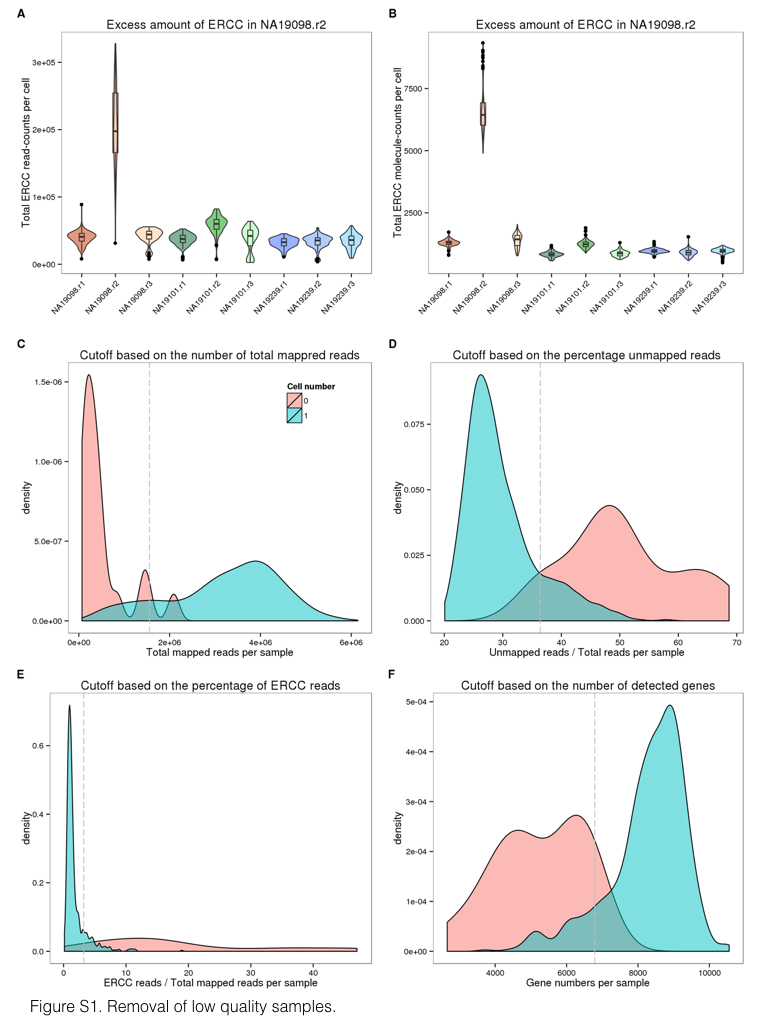
\includegraphics[trim=0 .5in 0 0,clip,width=5in]{img/ch04/Figure06.jpeg}
\caption[Removal of low quality
samples.]{\textbf{Removal of low quality
samples.} Violin plots of the total read-counts of ERCC spike-in
controls in (A) and the total molecule-counts in (B) in single cell
samples. The three colors represent the three individuals (NA19098 in
red, NA19101 in green, and NA19239 in blue). (C-F) Density plots of the
distributions of the total mapped reads in (C), the percentage of
unmapped reads in (D), the percentage of ERCC reads in (E), and the
number of detected genes in (F). The dash lines indicate the cutoffs
based on the 95th percentile of the samples with no cells.}
\label{fig:ch04-s1}
\end{figure}

\begin{figure}[!htb]
\centering
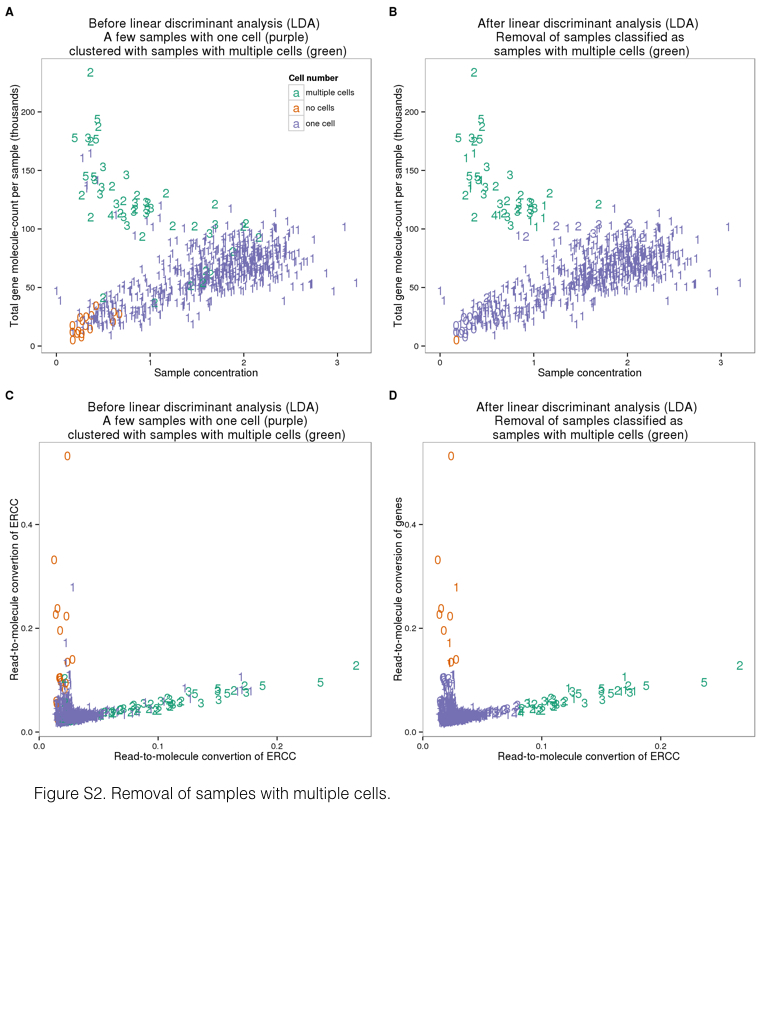
\includegraphics[trim=0 3.5in 0 0,clip,width=5in]{img/ch04/Figure07.jpeg}
\caption[Removal of samples with
multiple cells.]{\textbf{Removal of samples with
multiple cells.} Scatterplots of the three groups of samples (no cell in
green, single-cell in orange, and two or more cells in purple) before
(A) and after (B) the linear discriminant analysis (LDA) using sample
concentration of cDNA amplicons (ng/$\mu$l) and the number of detected
genes. (C and D) Similarly, LDA was performed to identify potential
multi-cell samples using the read-to-molecule conversion efficiency
(total molecule-counts divided by total read-counts per sample) of
endogenous genes and ERCC spike-in controls. Scatterplots of before and
after the LDA in (C) and (D), respectively. The numbers indicate the
number of cells observed in each cell capture site.}
\label{fig:ch04-s2}
\end{figure}

\begin{figure}[!htb]
\centering
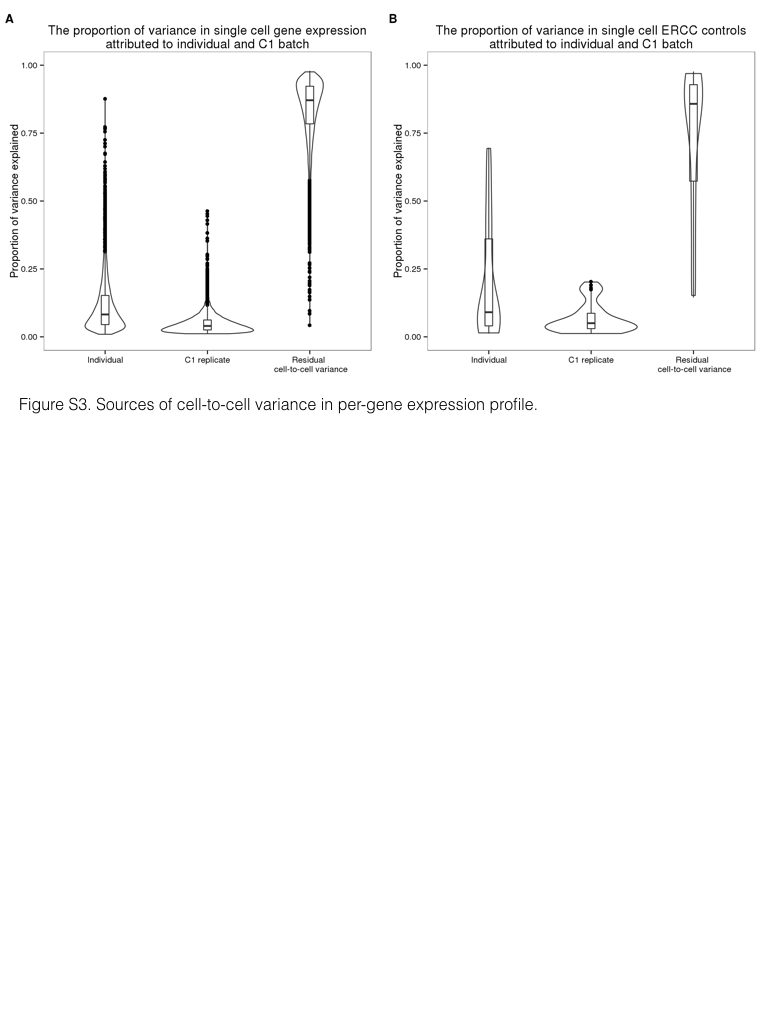
\includegraphics[trim=0 9in 0 0,clip,width=5in]{img/ch04/Figure08.jpeg}
\caption[Sources of cell-to-cell
variance in per-gene expression profile.]{\textbf{Sources of cell-to-cell
variance in per-gene expression profile.} Violin plots of the proportion
of per-gene cell-to-cell variance that was due to individual sample of
origin, different C1 replicates, and other single cell sample
differences. These results were calculated from the molecule counts
before normalization and batch correction. Endogenous genes are shown in
(A) and the ERCC spike-in controls in (B).}
\label{fig:ch04-s3}
\end{figure}

\begin{figure}[!htb]
\centering
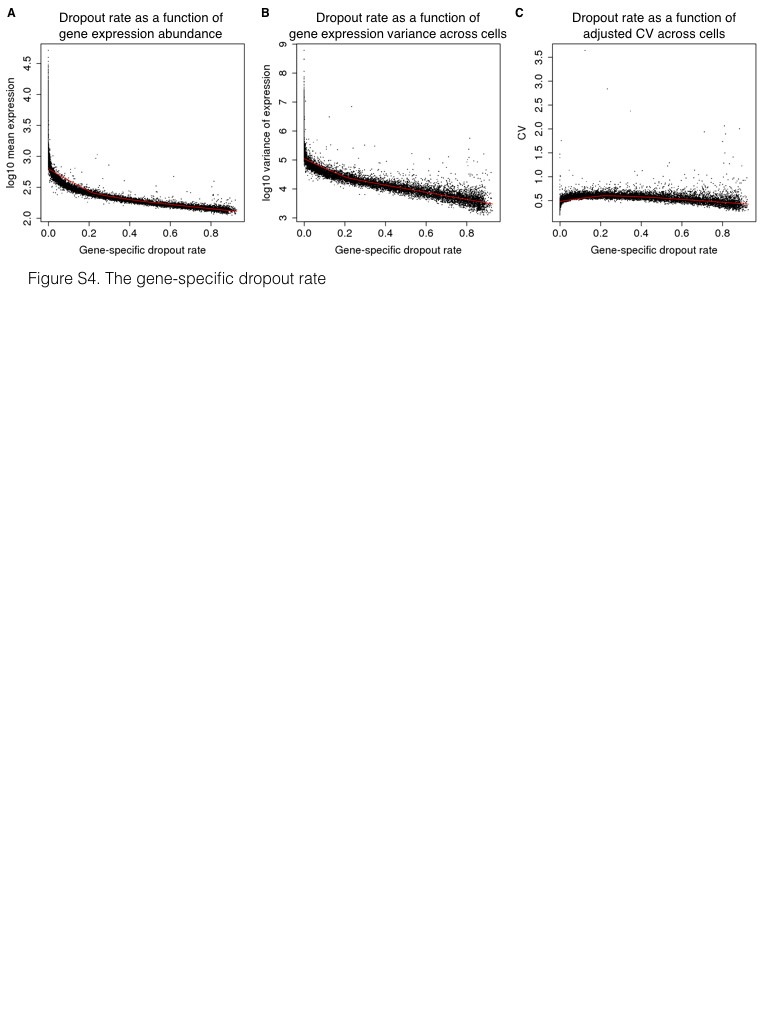
\includegraphics[trim=0 10.5in 0 0,clip,width=5in]{img/ch04/Figure09.jpeg}
\caption[The gene-specific dropout
rate.]{\textbf{The gene-specific dropout
rate.} The gene-specific dropout rate (the proportion of cells in which
the gene is undetected) and its relationship with log\textsubscript{10}
mean expression in (A), with log\textsubscript{10} variance of
expression in (B), and with the CV in (C) of the cells in which the gene
is expressed (cells in which at least one molecule of the given gene was
detected). Each point represents a gene, and red lines indicate the
predicted values using locally weighted scatterplot smoothing (LOESS).}
\label{fig:ch04-s4}
\end{figure}

\begin{figure}[!htb]
\centering
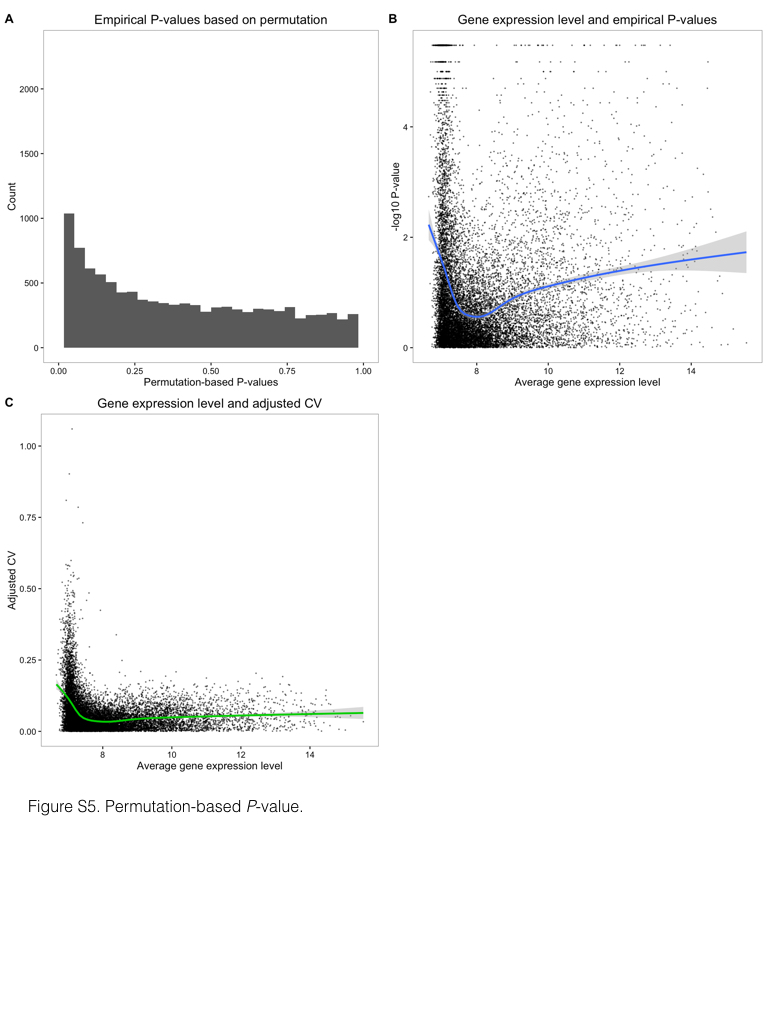
\includegraphics[trim=0 3.5in 0 0,clip,width=5in]{img/ch04/Figure10.jpeg}
\caption[Permutation-based
\emph{P}-value.]{\textbf{Permutation-based
\emph{P}-value.} (A) Histogram of empirical \emph{P}-values based on
300,000 permutations. (B) -log\textsubscript{10} empirical
\emph{P}-values are plotted against average gene expression levels. Blue
line indicates the fitted relationship between -log\textsubscript{10}
\emph{P}-values and average log\textsubscript{2} gene expression levels
of cells that were detected as expressed, using locally weighted
scatterplot smoothing (LOESS). (C) Median of Absolute Deviation (MAD) of
genes versus average gene expression levels. Green line indicates the
fitted relationship (LOESS) between the MAD values and average
log\textsubscript{2} gene expression levels of cells in which the gene
was detected as expressed.}
\label{fig:ch04-s5}
\end{figure}

\begin{figure}[!htb]
\centering
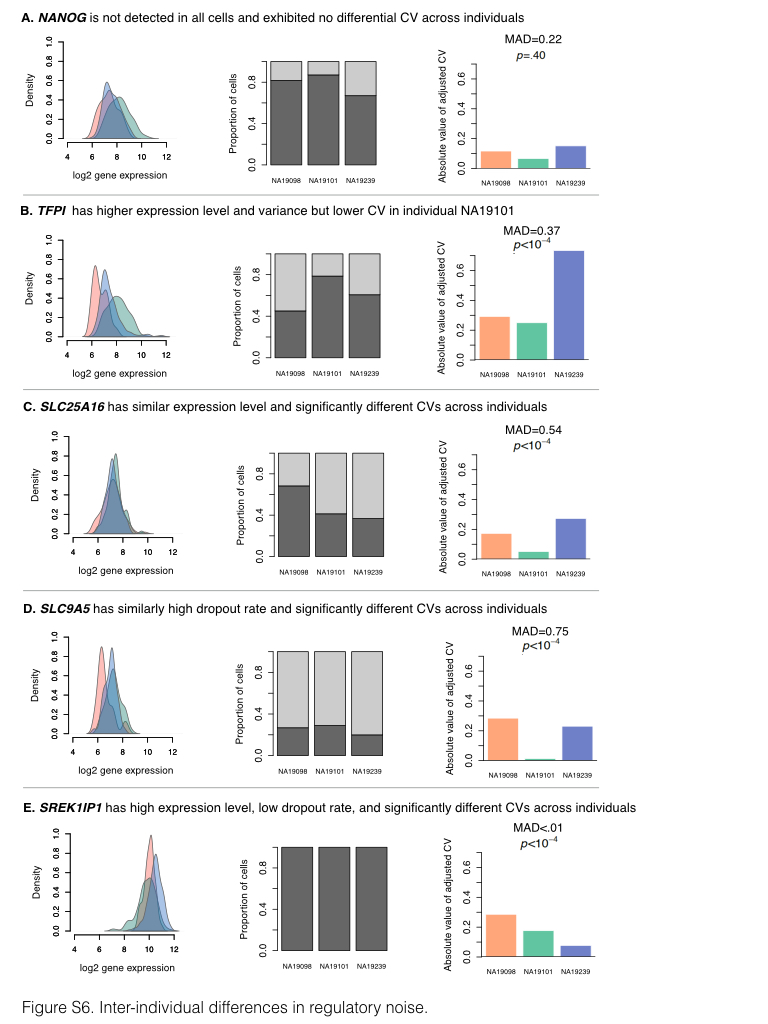
\includegraphics[trim=0 .5in 0 0,clip,width=5in]{img/ch04/Figure11.jpeg}
\caption[Inter-individual differences
in regulatory noise.]{\textbf{Inter-individual differences
in regulatory noise.} These 5 example genes illustrate various patterns
of cell-to-cell gene expression variance. For each gene, the left panel
shows the distribution of the log\textsubscript{2} gene expression
levels (considering only cells in which the gene is detected as
expressed), the middle panel shows the proportion of cells in which the
gene is detected as expressed (dark grey) and the dropout rate (light
grey) for each individual, and the right panel shows the absolute value
of adjusted CV for each individual, along with the corresponding
gene-specific MAD (median of absolute deviation) value and
\emph{P}-value. The three colors in the upper and lower panel represent
the individuals (NA19098 in red, NA19101 in green, and NA19239 in
blue).}
\label{fig:ch04-s6}
\end{figure}

\begin{figure}[!htb]
\centering
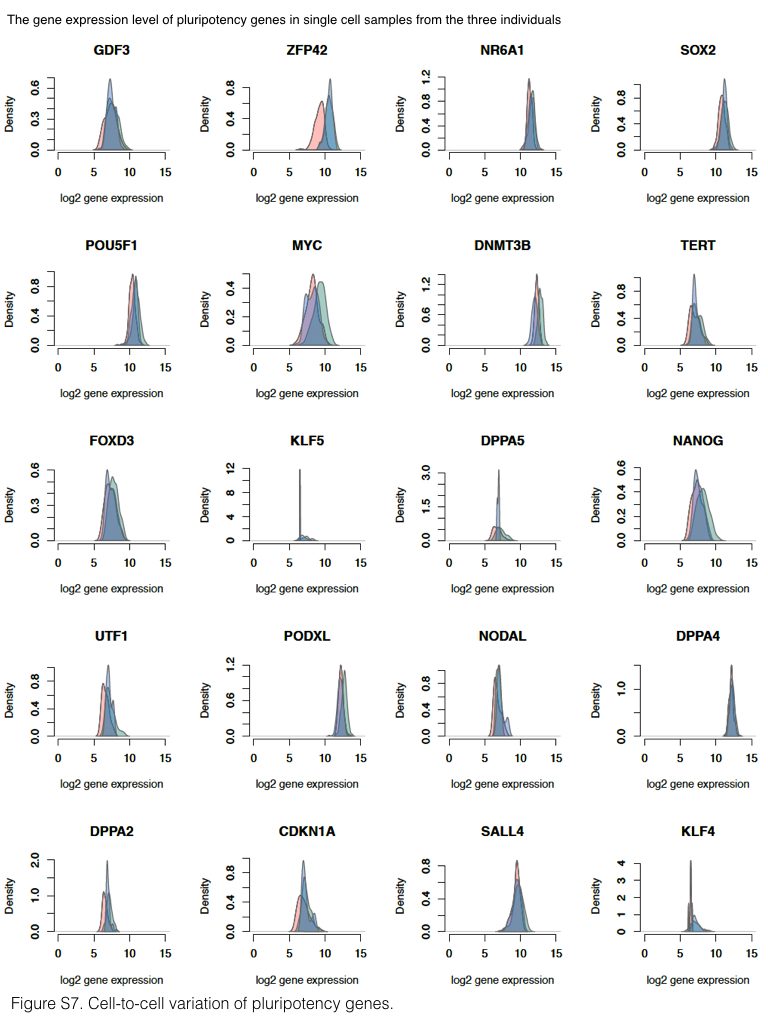
\includegraphics[trim=0 .5in 0 0,clip,width=5in]{img/ch04/Figure12.jpeg}
\caption[Cell-to-cell variation of
pluripotency genes.]{\textbf{Cell-to-cell variation of
pluripotency genes.} Density plots of the distribution of
log\textsubscript{2} gene expression of key pluripotency genes across
all single cells by individual. The peaks with lower gene expression
values (log2 around 4) represent the cells in which the gene is
undetected. The three colors represent the three individuals (NA19098 is
in red, NA19101 in green, and NA19239 in blue).}
\label{fig:ch04-s7}
\end{figure}

\begin{figure}[!htb]
\centering
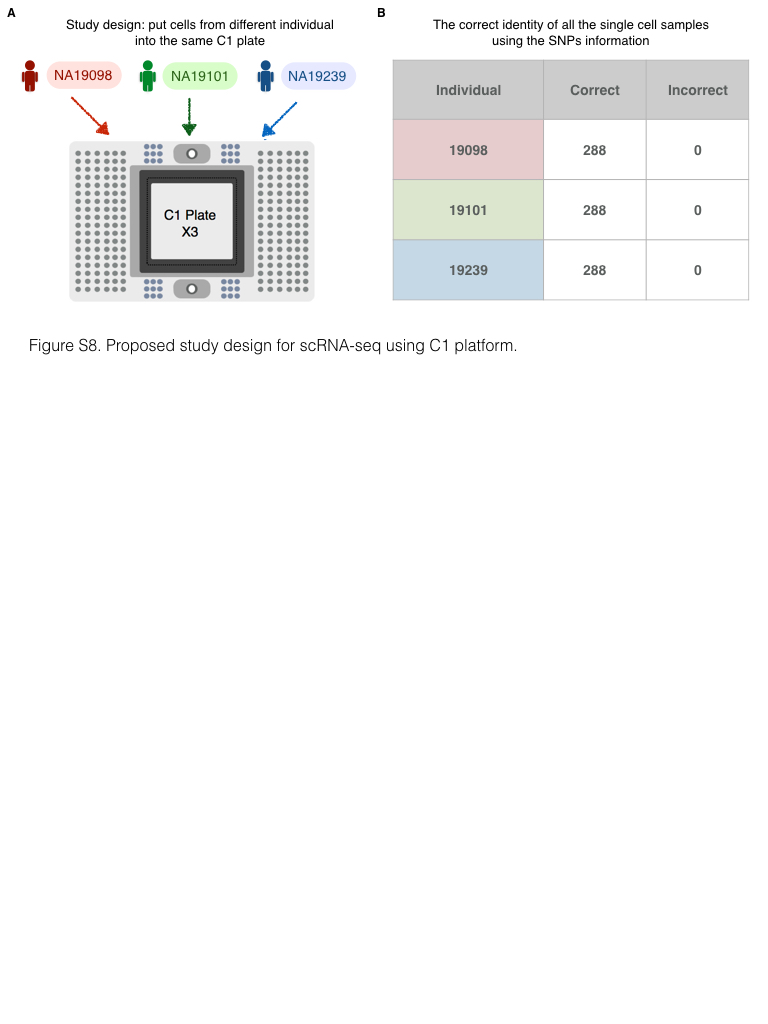
\includegraphics[trim=0 10in 0 0,clip,width=5in]{img/ch04/Figure13.jpeg}
\caption[Proposed study design for
scRNA-seq using C1 platform.]{\textbf{Proposed study design for
scRNA-seq using C1 platform.} (A) A balanced study design consisting of
multiple individuals within a C1 plate and multiple C1 replicates to
fully capture the batch effect across C1 plates and further retrieve the
maximum amount of biological information. (B) The correct identity of
each single cell sample was determined by examining the SNPs present in
their RNA sequencing reads.}
\label{fig:ch04-s8}
\end{figure}

\begin{figure}[!htb]
\centering
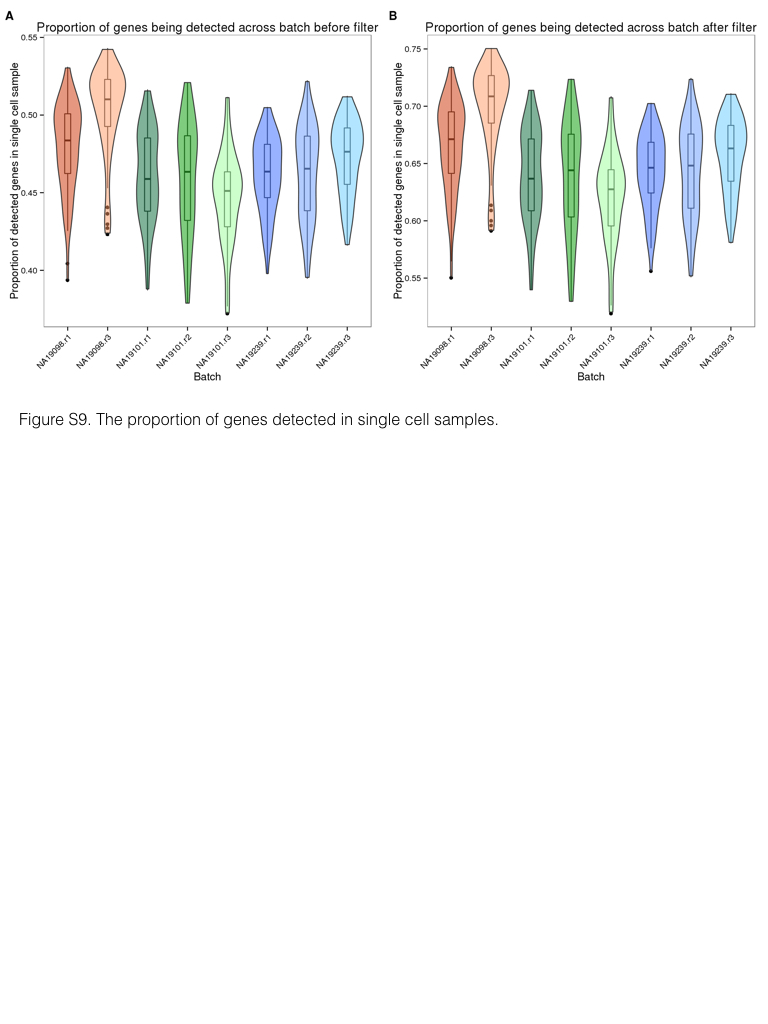
\includegraphics[trim=0 8.5in 0 0,clip,width=5in]{img/ch04/Figure14.jpeg}
\caption[The proportion of genes
detected in single cell samples.]{\textbf{The proportion of genes
detected in single cell samples.} Violin plots of the proportion of
genes detected, computed by the total number of detected genes in each
single cell divided by the total number of genes detected across all
single cells, before in (A) and after in (B) the removal of genes with
low expression. The three colors represent the three individuals
(NA19098 is in red, NA19101 in green, and NA19239 in blue).}
\label{fig:ch04-s9}
\end{figure}

\begin{figure}[!htb]
\centering
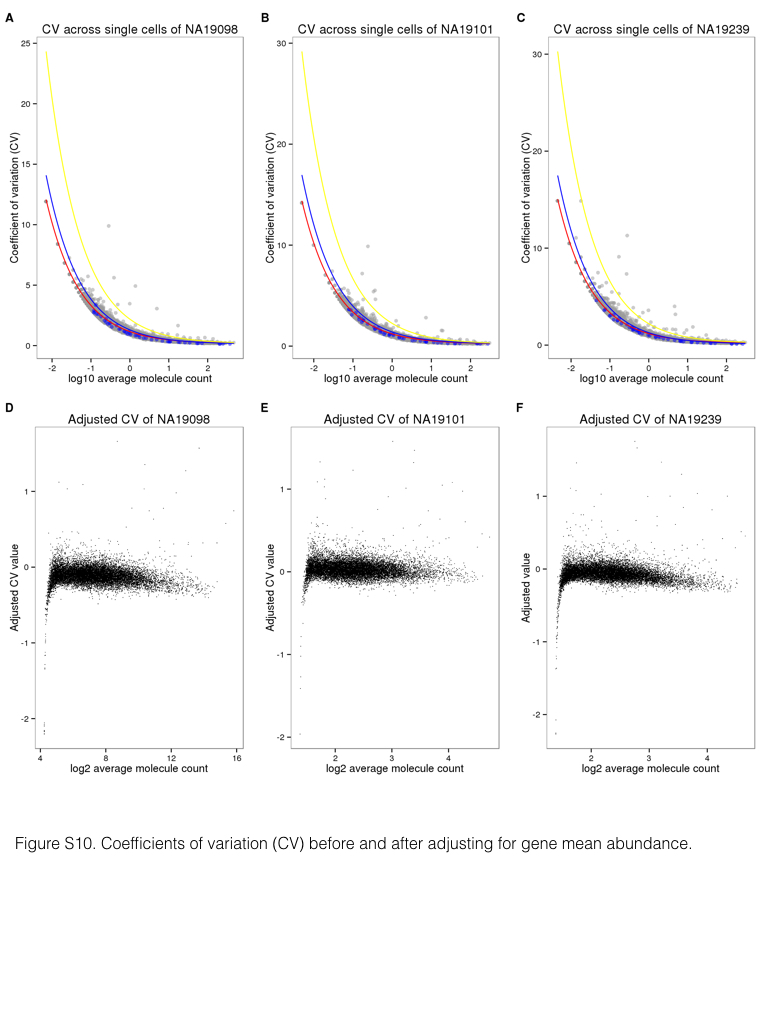
\includegraphics[trim=0 3in 0 0,clip,width=5in]{img/ch04/Figure15.jpeg}
\caption[Coefficients of variation
(CV) before and after adjusting for gene mean abundance.]{\textbf{Coefficients of variation
(CV) before and after adjusting for gene mean abundance.} (A-C) CV
plotted against average molecule counts across all cells for each
individual \citep{Islam2014}. Grey points represent endogenous genes, and
blue points represent ERCC spike-in controls. The curves indicate the
expected CV under three different scenarios. Red curve depicts the
expected CV of the endogenous genes while assuming a Poisson
distribution with no over-dispersion. Likewise, blue curve depicts the
expected CVs of the ERCC spike-in controls under the Poisson assumption.
Yellow curve depicts the expected CVs of an over-dispersed Poisson
distribution for which standard deviation is three times the ERCC
spike-in controls. (D-F) Adjusted CV values of each gene including all
cells are plotted against log\textsubscript{10} of the average molecule
counts for each individual.}
\label{fig:ch04-s10}
\end{figure}

\clearpage
\subsection{Supplementary Tables}\label{ch04-supplementary-tables}

\begin{table}[!htb]
\centering
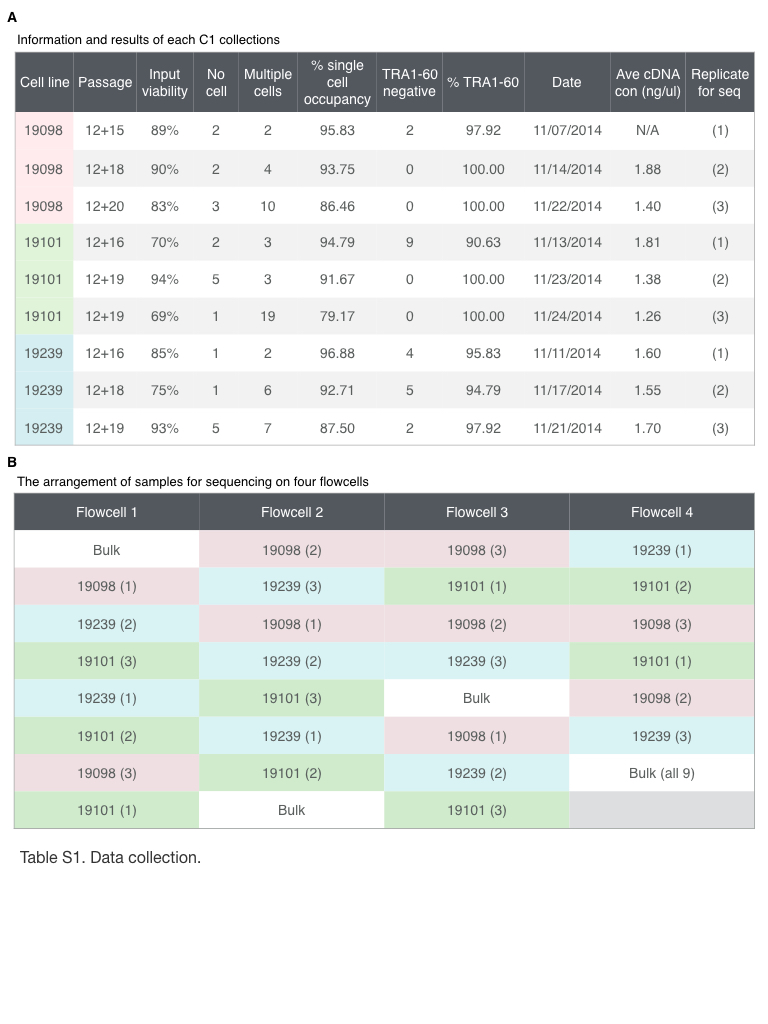
\includegraphics[trim=0 2.5in 0 0,clip,width=5in]{img/ch04/Figure16.jpeg}
\caption[Data collection.]{\textbf{Data collection.} (A) iPSCs were
 sorted using the 10-17 $\mu$m IFC plates with the staining of the
 pluripotency marker, TRA1-60. Single cell occupancy is the percentage
 of occupied capture sites containing one single cell. The average cDNA
 concentration was measured by the HT DNA high sensitivity LabChip
 (Caliper). (B) The 96 single cell libraries from one C1 plate were
 pooled and sequenced in three HiSeq lanes. The pooled samples were
 assigned across the four 8-lane flowcells.}
\label{tab:ch04-s1}
\end{table}
\clearpage

\begin{table}[!htb]
\caption[High quality single cell samples.]{\textbf{High quality single cell
samples.} (see supplementary file associated with this dissertation)
List of the 564 high quality single cell samples.}
\label{tab:ch04-s2}
\end{table}

\begin{table}[!htb]
\caption[Genes associated with inter-individual differences in regulatory noise.]{
\textbf{Genes associated with inter-individual differences in regulatory noise.}
 (see supplementary file associated with this dissertation) List of
 genes that we classified the estimates of regulatory noise as
 significantly different across individuals (empirical permutation
 \emph{P} \textless{} 10\textsuperscript{-4}). There are a total of 560
 genes.}
\label{tab:ch04-s3}
\end{table}

\begin{table}[!htb]
\caption[Gene ontology analysis of the genes associated with inter-individual
 differences in regulatory noise.]{\textbf{Gene ontology analysis of the
 genes associated with inter-individual differences in regulatory noise.}
 (see supplementary file associated with this dissertation)}
\label{tab:ch04-s4}
\end{table}


\chapter{Conclusion}\label{conclusion}

Traditional genetics approaches have been unable to identify variants
which can be used to predict susceptiblity to tuberculosis (TB),
likely due to the highly polygenic architecture of this complex trait
\citep{Thye2010, Mahasirimongkol2012, Thye2012, Png2012, Chimusa2014, Curtis2015, Sobota2016}.
Thus I performed experiments to interrogate a higher level phenotype,
gene expression levels, for which the effect of many variants of small
effect size can manifest in aggregrate. In my first approach, I
identified genes in innate immune cells whose gene expression levels
change in response to infection with \emph{Mycobacterium tuberculosis}
(MTB) but not other bacteria, highlighting their potential importance
for mycobacterial diseases \citep{Blischak2015}. In my second approach, I measured gene
expression levels in innate immune cells from individuals either
susceptible or resistant to develop active TB and built a
classifier to predict susceptibility to TB. These first two
experiments measured average gene expression levels across many
cells, and thus they missed any cell-to-cell heterogeneity in the innate
immune system \citep{Satija2014, Proserpio2016}. In my third approach, I established principles for the
effective design of studies to measure gene expression levels in
single cells \citep{Tung2016}. Given the success of my first two experiments, I expect
many more discoveries will be made by interrogating gene expression
measurements in single cells of the innate immune system.

\section{A joint Bayesian model provides a general framework for analyzing functional genomics studies with many conditions}

In Chapter \ref{ch:tb}, I described my work investigating the innate immune
response to MTB \citep{Blischak2015}. It is
known that the innate immune response is important for fighting MTB
infections \citep{Khan2016}. Alveolar macrophages are the primary target of MTB, and they
initiate the formation of granulomas to sequester MTB \citep{Sia2015}. Furthermore, vaccines
against TB have had limited efficacy \citep{Wang2013}. To identify human genes which are
important for the response to MTB infection, we isolated macrophages from six
healthy donors, infected them with MTB and other bacteria, and measured
genome-wide gene expression levels using RNA-seq at 4, 18, and 48 hours
post-infection.

Previous studies had identified genes which
are differentially expressed upon infection with MTB
\citep{Ehrt2001, Ragno2001, Nau2002, Chaussabel2003, Volpe2006, Tailleux2008}, and some have
even compared the differences between the reponse to strains of MTB
that vary in their virulence \citep{Coscolla2010, Wu2012}. The first novelty of our study was to
include many other bacteria in the infection experiments. Specifically, we
included the following mycobacteria: two strains of virulent MTB,
avirulent (heat-inavtivated) MTB, bacillus Calmette-Gu\'{e}rin (BCG; attentuated \emph{Mycobacterium
  bovis} used as a vaccine), and the avirulent \emph{Mycobacterium
  smegmatis}. The non-mycobacteria species we included were
\emph{Yersinia pseudotuberculosis}, \emph{Salmonella typhimurium}, and
\emph{Staphylococcus epidermidis}. This allowed us to distinguish
between the innate immune response to MTB versus other virulent
bacteria, MTB versus avirulent mycobacteria, amd MTB versus deceased
MTB.

This novel study design comparing many bacterial infections to isolate
the innate immune respone to MTB also posed analytical
challenges. The goal was to identify differences between the innate immune response
to each of the eight bacterial infections compared to the non-infected control condition.
Standard differential expression analyses (or in general
any large scale testing of thousands or more genomic features) are
well-suited for experiments with a few conditions \citep{Oshlack2010, Anders2013, Ritchie2015}. For example, the
most common approach is to perform pairwise differential expression
tests and then overlap the lists of differentially expressed
genes. In this instance, that would have meant peforming eight
pairwise tests to compare each bacterial infection to the control.
These results are always biased by incomplete power \citep{Ding2010, Flutre2013}. Because
hypothesis testing uses an arbitrary p-value threshold to determine
statistical significance, a gene with a p-value below this threshold
for one comparison but a p-value slightly above this threshold for a
separate comparison will be classified as specific to the first when
in reality the gene is behaving similarly in both. As the number of
pairwise comparisons increases, the problem of incomplete power is
exacerbated, i.e. a gene is more likely to be statistically
significant for some susbset of comparisons. This increase in
comparisons also decreases the ability to interpret the results. A
3-way Venn diagram (and perhaps a 4- or 5-way) can be interpreted, but
this approach breaks down with additional comparisons.

Another approach would be to directly compare the effect of infection between
two different groups of bacteria, e.g. compare the mean effect of infection  with mycobacteria versus the
mean effect of infection with non-mycobacteria (or virulent versus non-virulent bacteria). The advantage of this
approach is that it explicitly models the comparison and returns a p-value,
unlike the Venn diagram overlap approach. However, there are two main
downsides. First, statistical significance can be driven by outliers. For
example, in my study most of the significantly differentially expressed genes between
mycobacteria and non-mycobacteria were actually genes which were simply
differentially expressed in response to infection with \emph{S. typhimurium} and
\emph{S. epidermidis}. Second, this limits the potential results to the \emph{a priori}
ideas of the analyst and are not driven by the patterns in the actual data.

On the other end of the spectrum, a very data-driven approach would be to use a
clustering method such as hierarchical or k-means clustering \citep{Eisen1998, Michaels1998}. These multivariate
methods are able to find the patterns of gene expression in the data, both
expected and unexpected; however, since they are not accompanied by any formal
hypothesis test, it is difficult to interpret which clusters of co-expressed
genes are the most interesting to report.

Since none of the standard genomics approaches were adequate for properly
comparing 8 bacterial infections, I instead used a joint Bayesian model,
implemented in the software package Cormotif, to analyze the data \citep{Wei2015}. Conceptually,
Cormotif combines the clustering and pairwise testing approaches described
above. Just like the pairwise testing approach, the input to Cormotif are the
pairwise comparisons between each bacterial infection and the control
condition. However, to account for incomplete power, Cormotif models the gene
expression levels across all the pairwise comparisons to identify the main gene
expression patterns, conceptually similar to a clustering analysis.

The Cormotif results for my study were informative. Most of the genes were
either differentially expressed or not after infection with any of the
bacteria (Fig. \ref{fig:joint-all}). The two most interesting patterns in regards to understanding the
innate immune response to MTB were ``MTB'' and ``Virulent'' (Fig. \ref{fig:joint-18h},\ref{fig:joint-48h}).  The ``MTB'' pattern included
those genes which had a high posterior probability of being differentially
expressed in response to infection with MTB or closely related species and a medium posterior
probability of being differentially expressed in response to ifnection with \emph{M. smegmatis}, the
nonvirulent mycobacteria. The ``Virulent'' pattern included genes which had a high
posterior probability of being differentially expressed in response to infection
with any of the bacteria except heat-inactivated MTB or BCG.

In terms of better understanding TB susceptibility, the main takeaway from this
study was the identification of hundreds of genes which are differentially
expressed in response specifically to infection with MTB and related species but
not other virulent bacteria. These genes are candidates for containing genetic
variants which affect TB susceptibility. Furthermore, these genes could be
targets for future functional studies of how the innate immune system fights MTB
and also could give context to future results from genetic and functional
genomics studies of MTB infection. More generally, our methods are informative
to all future functional genomics studies. We were only able to confidently
isolate the effects of MTB infection by including multiple other bacterial
infections as comparison. Had we only infected the macrophages with MTB and
heat-inactivated MTB, we would have made multiple misclassifications. We would
have assigned differences between the two infections as specific to a live,
virulent MTB; however, these gene expression changes were also induced by other
live bacteria. Similarly, we would never have known that a subset of the genes
which were differentially expressed in response to both MTB and heat-inactivated
MTB were actually specific to mycobacteria in general. Not only was it important
to include multiple bacterial infections, but it was also critical to properly
analyze the results. Because the innate immune system is largely a general
response to infection, we expected most of the induced gene expression changes
to be similar across bacteria \citep{Huang2001, Boldrick2002, Nau2002, Jenner2005}.
Had we performed the straight-forward approach of
overlapping lists of differentially expressed genes from comparing the
individual infections to their controls, we would have had identified lots of
spurious differences in the innate immune response caused by incomplete
power. In contrast, by jointly modeling the data with Cormotif \citep{Wei2015}, we were able to
identify the shared gene expression patterns in response to related bacteria. In
support of the generality of this approach, the Cormotif approach was
successfully applied to distinguish the effects of vitamin D and bacterial
lipopolysaccharide on the innate immune response between individuals of
African-American and European-American ancestry (note: I was a co-author of the
study) \citep{Kariuki2016}.

It should be noted that this method also has its caveats. First, its strength of
sharing information across the pairwise comparisons can also be a negative
because it will not identify genes with unique expression patterns (Fig. \ref{fig:dusp14}). While useful
for projects with the aim of broadly characterizing the genome-wide gene
expression patterns for a given phenomenon, it is not well-suited for
identifying outlier genes. Second, because the algorithm is not deterministic,
Cormotif must be run multiple times to obtain the model with the highest log
likelihood. Because of this added complexity, using Cormotif is more difficult
to implement than more standard differential expression approaches.

\section{Initial success classifying individuals susceptible to tuberculsosis and future directions}

In Chapter \ref{ch:tb-suscept}, I described my work investigating the
role of gene regulation in the innate immune system on TB
susceptibility (not yet published). Specifically, in order to
investigate how the innate immune cells of susceptible individuals
function compared to those of resistant individuals, we collected
primary dendritic cells (DCs) from individuals that had recovered from
TB (i.e. susceptible) and individuals that tested positive for latent
TB infections but had not developed TB (i.e. resistant). We infected
the DCs with MTB and performed RNA sequencing (RNA-seq) on the infected and
non-infected cells.

There were three main conclusions from this work. First, the differences
in gene expression levels between resistant and susceptible
individuals were primarily present in the non-infected state and not 18
hours post-infection with MTB (Fig. \ref{fig:limma}). This suggests that these gene
expression differences primarily affect the very early response to MTB
infection. Second, we discovered that the effect sizes measured in our
\emph{in vitro} experiment, whether comparing between resistant and
susceptible individuals or between the infected and non-infected
states, were negatively correlated with lower p-values from two genome
wide association studies (GWAS) of TB susceptibility \citep{Thye2010} (Fig. \ref{fig:gwas}). This suggests
that our \emph{in vitro} system is a useful model for investigating
the genetic basis of TB susceptibility. Third, we trained a classifier
based on the gene expression levels in the non-infected state (Fig. \ref{fig:classifier}). Using
the threshold required to obtain a 100\% sensitivity (zero false negatives) in the
training data, we found that 11\% of healthy individuals from an
independent study \citep{Barreiro2012} were predicted to be susceptible to TB, very close
to the estimated population average of 10\% \citep{North2004, OGarra2013}. This suggests that
isolating innate immune cells and performing gene expression profiling
could be a feasible test for TB susceptibility.  The most obvious
extension of this work is to conduct a larger study with more
susceptible individuals. Our current results are only a
proof-of-principle. With a larger study, we could properly split the
data into training and test sets to assure that the model is not
overfitting the data. On the one hand, since we identified that the
gene expression differences are only present in the non-infected state
and that these are sufficient for the performance of the classifier,
this future study would be simplified by not having to perform the MTB
infections. On the other hand, collecting a large number of patient
samples is always difficult, and it is even worse when the individuals
are currently healthy and thus not regularly visiting the doctor like
those recovered from a past case of active TB. Hopefully these initial
successful results will provide the impetus for larger scale sample
collection.

Another fruitful direction for future experiments would be to further
investigate the role of \emph{CCL1} in the innate immune response to
MTB and its role in TB susceptibility. While studies of this gene have
had mixed results \citep{Thuong2008, Tang2011, Ozdemir2013},
all the studies, including my own \citep{Blischak2015}, have had small
sample sizes. In the first study of \emph{in vitro} differences in
gene expression between susceptible and resistant individuals,
\emph{CCL1} was found to be differentially expressed based on
susceptibility status \citep{Thuong2008}. Furthermore, the same study
found that SNPs nearby \emph{CCL1}were associated with TB
susceptibility in an independent cohort. In Chapter \ref{ch:tb}, I
found that \emph{CCL1} was one of the genes which changed expression
level specifically in response to infection with mycobacteria \citep{Blischak2015}. In
Chapter \ref{ch:tb-suscept}, I found that \emph{CCL1} was one of two
genes which had an effect size greater than 2 between susceptible and
resistant individuals in the non-infected state and also a p-value less
than 0.01 in two GWAS of TB susceptibility. There were many
differences between these studies (e.g. cell type, ethnicity of
donors, timepoints RNA was collected post-infection), yet \emph{CCL1}
was still a top hit in all three analyses. I believe this warrants
further investigation. As an example, one could use CRISPR/Cas \citep{Du2016} to
modify individual SNPs in THP-1 cells (a common cell line model of
monocytes) and test for differences in the response to MTB
infection. Another idea, since \emph{CCL1} is a secreted chemokine \citep{Miller1992},
would be to add varying amounts of exogenous \emph{CCL1} to the
\emph{in vitro} system to detect an effect on the innate immune
response.

\section{Incorporating lessons from single cell pilot study for future studies of the genetic basis of gene expression noise and the response to bacterial infection}

In Chapter \ref{ch:singleCellSeq}, I described my work on single cell
RNA-seq (scRNA-seq) \citep{Tung2016}. scRNA-seq is a relatively
new technique \citep{Liang2014, Macaulay2014, Saliba2014, Grun2015, Stegle2015, Bacher2016}
that enables the investigation of gene regulatory
changes at a much finer resolution than the bulk RNA-seq projects I
performed in Chapters \ref{ch:tb} and \ref{ch:tb-suscept}. While this
new technology is exciting, we must exercise the same caution as when
performing any large-scale genomics experiment \citep{Auer2010, Leek2010, Gilad2015}. Early studies of the
Fluidigm C1 system for scRNA-seq that focused on the technical sources
of variation largely focused on the variation from well-to-well within
just one C1 chip \citep{Brennecke2013, Grun2014, Islam2014, Ding2015, Vallejos2015}
; whereas, the studies investigating biological
phenomena tended to use multiple C1 chips without addressing the
obvious confounding batch effects (this problem is nicely highlighted
by \citep{Hicks2015}). Before conducting large scale scRNA-seq
experiments, we first aimed to better understand the technical factors
affecting the design of such studies. To do so, we performed scRNA-seq
of three C1 chip replicates of three HapMap \citep{HapMap2005} Yoruba individuals.

From these data, we learned many important lessons. First, by
performing subsampling analyses, we determined that sequencing
approximately 1.5 million reads for at least 75 cells from a given
individual was sufficient for detecting most expressed genes,
achieving a high correlation between the sum of the gene expression
levels across the single cells and the gene expression levels from
bulk sequencing of 10,000 cells, and achieving a high correlation
between the cell-to-cell variance in the gene expression levels across
the subset of single cells and the cell-to-cell variance measured in
all the single cells we collected for an individual (which ranged from
142 to 221) (Fig. \ref{fig:subsample}). Second, we observed technical variation introduced from
the processing of the C1 batches (Fig. \ref{fig:batch}). While this was expected, we also
observed unexpected aspects of this batch effect. The ERCC spike-in
controls which were added to each well and could potentially be used
to correct for this effect across C1 chips was affected not only by
technical variation but also by the biological variation (differences
between individuals) (Fig. \ref{fig:ch04-s3}). This entanglement of the technical and
biological sources of variation renders the spike-ins insufficient for
modeling technical variation between C1 chips (however they can still
be used to model technical variation between wells of the same C1
chip). This confounder occurred despite our use of unique molecular
identifiers (UMIs) to account for the bias introduced by amplifying
RNA from a small original source of just one cell \citep{Kivioja2011, Islam2014}. In fact, we found
that the conversion of reads to unique molecules was affected by
inter-individual differences (Fig. \ref{fig:batch}). Third, even with our small sample size
of only three individuals, we were able to identify inter-individual
differences in the cell-to-cell gene expression variance, or gene
expression noise (Fig. \ref{fig:variation}). This lends further support to the notion that gene
expression noise is a relevant factor that can affect biological
processes. Fourth, we demonstrated that we can use the single
nucleotide polymorphisms (SNPs) present in the RNA-seq reads to
identify the individual of origin for a given single cell \citep{Jun2012} (Fig. \ref{fig:ch04-s8}). This
enables us to use a crossed-design where single cells from multiple
individuals are included on the same C1 chip and later each well is
assigned to each individual based on the RNA-seq reads obtained. Our
initial nested design was inefficient because we collected hundreds of
single cells per individual across the multiple technical
replicates. From our subsampling we knew that collecting 75 high
quality single cells was sufficient. With a crossed design, we can
obtain about one C1 chip worth of wells (96) while still modeling the
technical variation across C1 chips.

Given the promising results from our first study, our next study will
aim to further investigate the impact of genetic variation on gene
expression noise by measuring single cell gene expression levels in 60
individuals. The design of the study is informed by our previous
findings. First, we will put single cells from multiple individuals on
each C1 chip because we know we can identify the individual based on
the RNA-seq reads. Second, we will repeat each individual across C1
chips until they obtain on average 96 wells (e.g. one C1 chip) because
this will get us close to our target of 75 single cells after removing
low quality cells. Third, we will replace the ERCC spike-ins with RNA
from a distantly related model organism. With many more technical
spike-ins gene to measure, these will be more useful for modeling
technical variation \citep{Risso2014}. Using this study design, we'll
be able to efficiently measure gene expression noise from many
individuals while still properly accounting for technical variation.

Returning to the \emph{in vitro} models of bacterial infection from my
other studies, I can imagine future single cell studies that shed
further light on the innate immune response. While we infect the cells
at a multiplicity of infection of 1:1, some cells will still be
infected by multiple bacteria and others not infected at
all. Furthermore, there could be variation in this distribution of the
number of bacteria per cell across individuals. In order to
efficiently measure single cell gene expression in response to
infection, I would put uninfected cells from one individual on the
same C1 chip as the infected cells from a different individual. Also,
since the MTB H37Rv strain we typically use has a GFP tag, we could
use high-throughput fluorescence microscopy of each well to count the
number of bacteria per cell. With this high resolution data, we could
differentiate between inter-individual differences in the innate
immune response due to differences in the number of infected cells (or
the number of bacteria per cell) or differences in the innate immune
response in the infected cells.

\section{The importance of mitigating batch effects in any genomics experiment}

A common theme of all my projects is accounting for technical
biases. Although only Chapter \ref{ch:singleCellSeq} has a main focus
on mitigating batch effects, all my projects required close attention
to this problem. This is because all genomics studies need to account
for batch effects in both the design and analysis of the data,
otherwise the results are meaningless \citep{Auer2010, Leek2010, Gilad2015}. There will be signal in any large
data set, but it will only inform biological insight if the signal
arises from the biological processes being studied.

In Chapter \ref{ch:tb}, we collected a total of 156 RNA-seq
samples. During the batch processing, we ensured that the biological
factors of interest (bacterial infection, timepoint, individual) were
balanced to avoid introducing spurious signal. Furthermore, upon data
exploration, we observed that the processing batch and the RNA quality
score (RIN) were correlated with the first principal component (PC) (Fig. \ref{fig:pca}). After
regressing these two variables, the first PC was the
effect of timepoint and the second PC was the effect of
infection. Importantly, we obtained similar results with or without
protecting the variables of interest in the linear model when
regressing out the technical variables. This was a result of the careful
planning of the batch processing to avoid confounding biological and
technical variables.

In Chapter \ref{ch:tb-suscept}, I once again designed the batch
processing to balance the biological factors of interest
(susceptibility status, treatment, individual) (Fig. \ref{fig:process}). Conveniently, this
project did not have large scale batch effects (Fig. \ref{fig:batch-effect}), likely due to the
smaller overall sample size of 48. However, accounting for a batch
effect was critical for training a classifier on the current data set
and testing it on an independent data set \citep{Barreiro2012}.
Not only were the studies
performed years apart, but the gene expression levels were measured
using different technologies. Thus I was only able to compare the two
studies after normalizing each sample (Fig. \ref{fig:combined-dist}) and removing the large batch
effect by regressing the first PC of the combined
data set (Fig. \ref{fig:combined-pca}). Testing the classifier without accounting for the batch
effect would have given poor results simply due to technical reasons.

In Chapter \ref{ch:singleCellSeq}, one of the main motivations for the
study was understanding the magnitude of the batch effect of
collecting scRNA-seq on separate C1 chips. While the technical effect
of C1 batch was smaller in magnitude compared to the biological effect
of individual (assessed using variance components analysis) (Fig. \ref{fig:ch04-s3}), not
including technical replicates would attribute the substantial
technical effect to the biological effect. Just as we require
replication for established genomic protocols, it is also necessary to
replicate scRNA-seq experiments, especially since the standard ERCC
spike-ins appear to be affected by both biological and technical
factors. Fortunately, we were able to devise a strategy to reduce the
required number of C1 replicates by combining single cells from
multiple individuals onto each C1 chip and then replicating the
multiple individuals across multiple chips (Fig. \ref{fig:ch04-s8}). This crossed design
accounts for batch effects while minimizing the required replication.

In summary, technical batch effects need to be considered from the
initial design of a genomics experiments through to the data analysis
and interpretation of the results.

\section{Concluding remarks}

First, I have identified hundreds of genes specifically involved in
fighting MTB infections. More broadly, I have demonstrated that a
joint Bayesian model is an effective tool for analyzing the results of
genomic studies with many conditions. Second, I have demonstrated that
the gene expression levels in non-infected DCs may be able to predict
susceptiblity to TB. Third, I have determined an effective study
design for future single cell studies that accounts for technical
batch effects while simultaneously decreasing the necessary sample
size. Overall my results are informative not only for understanding
how differences in the innate immune response confer susceptibility or
resistance to TB, but also inform the design and analysis of any
functional genomics experiment.


% Format a LaTeX bibliography
\makebibliography

% Figures and tables, if you decide to leave them to the end
%\input{figure}
%\input{table}

\end{document}


